% Options for packages loaded elsewhere
\PassOptionsToPackage{unicode}{hyperref}
\PassOptionsToPackage{hyphens}{url}
\PassOptionsToPackage{dvipsnames,svgnames,x11names}{xcolor}
%
\documentclass[
  letterpaper,
  xelatex,
  ja=standard, xelatex]{bxjsbook}

\usepackage{amsmath,amssymb}
\usepackage{iftex}
\ifPDFTeX
  \usepackage[T1]{fontenc}
  \usepackage[utf8]{inputenc}
  \usepackage{textcomp} % provide euro and other symbols
\else % if luatex or xetex
  \usepackage{unicode-math}
  \defaultfontfeatures{Scale=MatchLowercase}
  \defaultfontfeatures[\rmfamily]{Ligatures=TeX,Scale=1}
\fi
\usepackage{lmodern}
\ifPDFTeX\else  
    % xetex/luatex font selection
\fi
% Use upquote if available, for straight quotes in verbatim environments
\IfFileExists{upquote.sty}{\usepackage{upquote}}{}
\IfFileExists{microtype.sty}{% use microtype if available
  \usepackage[]{microtype}
  \UseMicrotypeSet[protrusion]{basicmath} % disable protrusion for tt fonts
}{}
\makeatletter
\@ifundefined{KOMAClassName}{% if non-KOMA class
  \IfFileExists{parskip.sty}{%
    \usepackage{parskip}
  }{% else
    \setlength{\parindent}{0pt}
    \setlength{\parskip}{6pt plus 2pt minus 1pt}}
}{% if KOMA class
  \KOMAoptions{parskip=half}}
\makeatother
\usepackage{xcolor}
\usepackage[no]{geometry}
\setlength{\emergencystretch}{3em} % prevent overfull lines
\setcounter{secnumdepth}{5}
% Make \paragraph and \subparagraph free-standing
\ifx\paragraph\undefined\else
  \let\oldparagraph\paragraph
  \renewcommand{\paragraph}[1]{\oldparagraph{#1}\mbox{}}
\fi
\ifx\subparagraph\undefined\else
  \let\oldsubparagraph\subparagraph
  \renewcommand{\subparagraph}[1]{\oldsubparagraph{#1}\mbox{}}
\fi

\usepackage{color}
\usepackage{fancyvrb}
\newcommand{\VerbBar}{|}
\newcommand{\VERB}{\Verb[commandchars=\\\{\}]}
\DefineVerbatimEnvironment{Highlighting}{Verbatim}{commandchars=\\\{\}}
% Add ',fontsize=\small' for more characters per line
\usepackage{framed}
\definecolor{shadecolor}{RGB}{241,243,245}
\newenvironment{Shaded}{\begin{snugshade}}{\end{snugshade}}
\newcommand{\AlertTok}[1]{\textcolor[rgb]{0.68,0.00,0.00}{#1}}
\newcommand{\AnnotationTok}[1]{\textcolor[rgb]{0.37,0.37,0.37}{#1}}
\newcommand{\AttributeTok}[1]{\textcolor[rgb]{0.40,0.45,0.13}{#1}}
\newcommand{\BaseNTok}[1]{\textcolor[rgb]{0.68,0.00,0.00}{#1}}
\newcommand{\BuiltInTok}[1]{\textcolor[rgb]{0.00,0.23,0.31}{#1}}
\newcommand{\CharTok}[1]{\textcolor[rgb]{0.13,0.47,0.30}{#1}}
\newcommand{\CommentTok}[1]{\textcolor[rgb]{0.37,0.37,0.37}{#1}}
\newcommand{\CommentVarTok}[1]{\textcolor[rgb]{0.37,0.37,0.37}{\textit{#1}}}
\newcommand{\ConstantTok}[1]{\textcolor[rgb]{0.56,0.35,0.01}{#1}}
\newcommand{\ControlFlowTok}[1]{\textcolor[rgb]{0.00,0.23,0.31}{#1}}
\newcommand{\DataTypeTok}[1]{\textcolor[rgb]{0.68,0.00,0.00}{#1}}
\newcommand{\DecValTok}[1]{\textcolor[rgb]{0.68,0.00,0.00}{#1}}
\newcommand{\DocumentationTok}[1]{\textcolor[rgb]{0.37,0.37,0.37}{\textit{#1}}}
\newcommand{\ErrorTok}[1]{\textcolor[rgb]{0.68,0.00,0.00}{#1}}
\newcommand{\ExtensionTok}[1]{\textcolor[rgb]{0.00,0.23,0.31}{#1}}
\newcommand{\FloatTok}[1]{\textcolor[rgb]{0.68,0.00,0.00}{#1}}
\newcommand{\FunctionTok}[1]{\textcolor[rgb]{0.28,0.35,0.67}{#1}}
\newcommand{\ImportTok}[1]{\textcolor[rgb]{0.00,0.46,0.62}{#1}}
\newcommand{\InformationTok}[1]{\textcolor[rgb]{0.37,0.37,0.37}{#1}}
\newcommand{\KeywordTok}[1]{\textcolor[rgb]{0.00,0.23,0.31}{#1}}
\newcommand{\NormalTok}[1]{\textcolor[rgb]{0.00,0.23,0.31}{#1}}
\newcommand{\OperatorTok}[1]{\textcolor[rgb]{0.37,0.37,0.37}{#1}}
\newcommand{\OtherTok}[1]{\textcolor[rgb]{0.00,0.23,0.31}{#1}}
\newcommand{\PreprocessorTok}[1]{\textcolor[rgb]{0.68,0.00,0.00}{#1}}
\newcommand{\RegionMarkerTok}[1]{\textcolor[rgb]{0.00,0.23,0.31}{#1}}
\newcommand{\SpecialCharTok}[1]{\textcolor[rgb]{0.37,0.37,0.37}{#1}}
\newcommand{\SpecialStringTok}[1]{\textcolor[rgb]{0.13,0.47,0.30}{#1}}
\newcommand{\StringTok}[1]{\textcolor[rgb]{0.13,0.47,0.30}{#1}}
\newcommand{\VariableTok}[1]{\textcolor[rgb]{0.07,0.07,0.07}{#1}}
\newcommand{\VerbatimStringTok}[1]{\textcolor[rgb]{0.13,0.47,0.30}{#1}}
\newcommand{\WarningTok}[1]{\textcolor[rgb]{0.37,0.37,0.37}{\textit{#1}}}

\providecommand{\tightlist}{%
  \setlength{\itemsep}{0pt}\setlength{\parskip}{0pt}}\usepackage{longtable,booktabs,array}
\usepackage{calc} % for calculating minipage widths
% Correct order of tables after \paragraph or \subparagraph
\usepackage{etoolbox}
\makeatletter
\patchcmd\longtable{\par}{\if@noskipsec\mbox{}\fi\par}{}{}
\makeatother
% Allow footnotes in longtable head/foot
\IfFileExists{footnotehyper.sty}{\usepackage{footnotehyper}}{\usepackage{footnote}}
\makesavenoteenv{longtable}
\usepackage{graphicx}
\makeatletter
\def\maxwidth{\ifdim\Gin@nat@width>\linewidth\linewidth\else\Gin@nat@width\fi}
\def\maxheight{\ifdim\Gin@nat@height>\textheight\textheight\else\Gin@nat@height\fi}
\makeatother
% Scale images if necessary, so that they will not overflow the page
% margins by default, and it is still possible to overwrite the defaults
% using explicit options in \includegraphics[width, height, ...]{}
\setkeys{Gin}{width=\maxwidth,height=\maxheight,keepaspectratio}
% Set default figure placement to htbp
\makeatletter
\def\fps@figure{htbp}
\makeatother

\usepackage{booktabs}
%\setjamonofont{SourceHanCodeJP-Light}
%\XeTeXgenerateactualtext=1
\usepackage{tikz}
\usepackage{makeidx}
\makeindex
\makeatletter
\@ifpackageloaded{bookmark}{}{\usepackage{bookmark}}
\makeatother
\makeatletter
\@ifpackageloaded{caption}{}{\usepackage{caption}}
\AtBeginDocument{%
\ifdefined\contentsname
  \renewcommand*\contentsname{目次}
\else
  \newcommand\contentsname{目次}
\fi
\ifdefined\listfigurename
  \renewcommand*\listfigurename{図一覧}
\else
  \newcommand\listfigurename{図一覧}
\fi
\ifdefined\listtablename
  \renewcommand*\listtablename{表一覧}
\else
  \newcommand\listtablename{表一覧}
\fi
\ifdefined\figurename
  \renewcommand*\figurename{図}
\else
  \newcommand\figurename{図}
\fi
\ifdefined\tablename
  \renewcommand*\tablename{表}
\else
  \newcommand\tablename{表}
\fi
}
\@ifpackageloaded{float}{}{\usepackage{float}}
\floatstyle{ruled}
\@ifundefined{c@chapter}{\newfloat{codelisting}{h}{lop}}{\newfloat{codelisting}{h}{lop}[chapter]}
\floatname{codelisting}{コード}
\newcommand*\listoflistings{\listof{codelisting}{コード一覧}}
\makeatother
\makeatletter
\makeatother
\makeatletter
\@ifpackageloaded{caption}{}{\usepackage{caption}}
\@ifpackageloaded{subcaption}{}{\usepackage{subcaption}}
\makeatother
\ifLuaTeX
\usepackage[bidi=basic]{babel}
\else
\usepackage[bidi=default]{babel}
\fi
\babelprovide[main,import]{japanese}
% get rid of language-specific shorthands (see #6817):
\let\LanguageShortHands\languageshorthands
\def\languageshorthands#1{}
\ifLuaTeX
  \usepackage{selnolig}  % disable illegal ligatures
\fi
\usepackage{bookmark}

\IfFileExists{xurl.sty}{\usepackage{xurl}}{} % add URL line breaks if available
\urlstyle{same} % disable monospaced font for URLs
\hypersetup{
  pdftitle={R と RStudio},
  pdfauthor={宮﨑憲治},
  pdflang={ja-JP},
  colorlinks=true,
  linkcolor={blue},
  filecolor={Maroon},
  citecolor={Blue},
  urlcolor={Blue},
  pdfcreator={LaTeX via pandoc}}

\title{R と RStudio}
\author{宮﨑憲治}
\date{2025-10-25}

\begin{document}
\maketitle

\renewcommand*\contentsname{目次}
{
\hypersetup{linkcolor=}
\setcounter{tocdepth}{2}
\tableofcontents
}
\bookmarksetup{startatroot}

\chapter{R と RStudio}\label{r-ux3068-rstudio}

\bookmarksetup{startatroot}

\chapter*{はじめに}\label{ux306fux3058ux3081ux306b}
\addcontentsline{toc}{chapter}{はじめに}

\markboth{はじめに}{はじめに}

\section{R とは}\label{r-ux3068ux306f}

Rは統計・データ解析・統計グラフ作成のためのオープンソースソフトである.
基本的に無料で使える.
最近はその統合環境であるRStudioがデファクトスタンダードとなっている.
さらにそれらは RStudio Cloud (https://rstudio.cloud/)
としてクラウド環境でも使用できる.
ここではまずローカル環境でR言語をいれる方法を解説する.
第2節にRStudioのローカル環境での導入方法を述べる.

RStudio
Cloud については直接サイトに行き,そのヘルプを見て導入すれば良いだろう.
日本語の解説としては以下が参考になるだろう.

https://qiita.com/ZaKama/items/937e6d7fa25f6d3cb385

\section{R
のインストール}\label{r-ux306eux30a4ux30f3ux30b9ux30c8ux30fcux30eb}

Rをインストールするには

https://cran.r-project.org/

にいき, 該当機種のファイルをダウンロードする.
ダウンロードしたあとに実行すればインストールされる.

Windows の場合, 32bit か 64bit を選択する. 最近のパソコンの CPU は 64bit
と考えられるが, どちらかわからなければ 32bit にしておけばよい.

Ubuntu なら \texttt{ppa} を使って導入してもよい.

\begin{verbatim}
sudo add-apt-repository ppa:marutter/rrutter
sudo apt-get update
sudo apt-get install r-base r-base-dev
\end{verbatim}

\section{R の設定}\label{r-ux306eux8a2dux5b9a}

設定ファイル \texttt{.Rprofile} をホームディレクトリに作成すれば,
設定を変更できる. ホームディレクトリはユーザー名が \texttt{kenji}
のとき, Windows なら通常
\texttt{C:\textbackslash{}Users\textbackslash{}kenji} である.
バックスラッシュ \texttt{\textbackslash{}} は \(\yen\)
と読み替えて頂きたい. 最初は \texttt{.Rprofile}
を特に作成しなくても大丈夫である.

Windowsを利用して日本語のユーザー名を使用している場合に使えない.
Rを実施するためのユーザー名を別に作成するか,アカウント名を変えた方がよいだろう.
なお日本語ユーザー名のままファイルパスを英語化するには以下を参考されたい:

https://clean-copy-of-onenote.hatenablog.com/entry/R\_japanese\_username

\section{R の使い方}\label{r-ux306eux4f7fux3044ux65b9}

Windows だとコマンドプロンプトから R と入力して立ち上げるか, R
のアイコンをダブルクリックすると, Rコンソールと言われる画面が現れる.
コマンドプロンプトからだと最初の表示が文字化けしている可能性があるが,
その後の起動に問題ないはずである. アイコンがなければ, Winキーを押した後,
\texttt{rgui} と入力すれば起動できる. Mac や Ubuntu だとターミナルから R
と入力して起動できる.

立ち上げた後, コンソールから そこにコマンドを入力すると,
その結果が直後に出力される. 終了には \texttt{q()} とする.
作業スペースを保存するかと聞かれたなら, No を意味する \texttt{n}
を選択する.

コマンド入力中, 最後の括弧を付け忘れたり,
正しく実行ができないときがある. たとえば, \texttt{rnorm(5}
としてEnterキーを押せば, 次の行に \texttt{+} とでてくる. ここでは正しく
\texttt{)} を付けて再度Enterキーを押せば正しく実行されるが,
ときにはどれを入力すれば正しく実行されるかわからない一方で,
単にEnterを押すだけだと, 再度入力を求められることがある.
そうしたとときは通常左上にあるエスケープキー (ESC)
を押せば途中入力がキャンセルされる.

R はRコンソールから対話式にコマンドを入力していく方法と, 拡張子
\texttt{R} のスクリプトファイルを実行していくやり方がある.
実行履歴を記録するためにスクリプトファイルを作成していくやり方を推奨する.

スクリプトファイル \texttt{project.R} を Rコンソールから実行するには,

\begin{verbatim}
source("project.R")
\end{verbatim}

とすればよい.

R外部のコマンドプロンプトから実行するには

\begin{verbatim}
Rscript project.R
\end{verbatim}

とすればよい. 起動できないときには, 環境変数の PATH
にRの実行ファイルの場所が登録されていない可能性がある.

また外部ファイルを導入する際やファイルを外部出力する際には,
現在の作業ディレクトリに気をつけなければならない.
現在の作業ディレクトリの場所はRコンソールから

\begin{verbatim}
getwd()
\end{verbatim}

とすれば, 確認できる. Windows
だと通常の表記と異なっていることに注意されたい.

作業ディレクトリの指定は以下のようにする.

\begin{verbatim}
setwd(PATH)
\end{verbatim}

Windows のとき指定の仕方に注意が必要である. たとえば作業ディレクトリが
\texttt{C:\textbackslash{}Users\textbackslash{}kenji\textbackslash{}work\textbackslash{}project}
のとき,

\begin{verbatim}
setwd("C:/Users/kenji/work/project")
\end{verbatim}

となる. バックスラッシュ \texttt{\textbackslash{}} (\(\yen\)) を
スラッシュ \texttt{/} に変更しなければならない.

\bookmarksetup{startatroot}

\chapter{R の基本}\label{r-ux306eux57faux672c}

R の基礎を学ぶには、次のオンライン教材が役立つ(2025 年時点)。

\begin{itemize}
\tightlist
\item
  Posit Cloud Primers(旧 RStudio Primers)\\
  https://posit.cloud/learn/primers\\
  インタラクティブな演習を通じて R の基礎から tidyverse
  まで幅広く学べる。英語のみの提供だが、無料アカウントで主要コンテンツを利用できる。
\item
  Posit Academy\\
  https://academy.posit.co/\\
  Posit 社が提供する体系的な e
  ラーニングプログラム。動画とハンズオン課題で R
  とデータサイエンスを段階的に学べる(英語、要アカウント)。
\item
  swirl(R コンソール内で動作する対話型チュートリアル)\\
  https://swirlstats.com/\\
  R
  のコンソールに組み込んで利用する教材で、コマンドを入力しながら学習できる。コミュニティ制作のレッスンには日本語訳もある。
\item
  R for Data Science, 2nd Edition(オンライン書籍)\\
  https://r4ds.hadley.nz/\\
  R と tidyverse のモダンな実践書。ブラウザで無料公開され、Posit Cloud
  のサンプルプロジェクトからコードをすぐ試せる。
\end{itemize}

日本語で要点を確認したい場合は、以下のリソースが便利である。

\begin{itemize}
\tightlist
\item
  R for Data Science 日本語版(第 1 版)\\
  https://r4ds-jp.netlify.app/\\
  コミュニティによる翻訳。基礎からデータ可視化、tidyverse
  の使い方まで日本語で学べる。
\item
  Posit のチートシート集\\
  https://posit.co/resources/cheatsheets/\\
  公式の英語版に加え、従来の日本語版 PDF(例:
  https://www.rstudio.com/wp-content/uploads/2016/10/r-cheat-sheet-ja.pdf)も引き続き利用できる。
\item
  統計 Web(統計数理研究所による解説サイト)\\
  https://statistics.co.jp/learning/\\
  R の導入から基本操作、グラフ作成までを日本語で丁寧に解説している。
\end{itemize}

動画教材としては、ドットインストールの「はじめての R
プログラミング」講座(13 本、合計約 40 分)が 2024
年以降も公開されており、基本編は無料で視聴できる。 

http://dotinstall.com/lessons/basic\_r

このほかにも、Posit 公式チャンネルや国内コミュニティが公開する YouTube
動画が随時更新されているため、興味のあるトピックで検索してみるとよい。

\section{電卓としての R}\label{ux96fbux5353ux3068ux3057ux3066ux306e-r}

R は電卓としても利用できる。 代表的な算術演算子を以下に示す。

\begin{longtable}[]{@{}lll@{}}
\toprule\noalign{}
演算子 & 説明 & 例 \\
\midrule\noalign{}
\endhead
\bottomrule\noalign{}
\endlastfoot
\texttt{+} & 足し算 & \texttt{5\ +\ 2\ =\ 7} \\
\texttt{-} & 引き算 & \texttt{5\ -\ 2\ =\ 3} \\
\texttt{*} & 掛け算 & \texttt{5\ *\ 2\ =\ 10} \\
\texttt{/} & 割り算 & \texttt{5\ /\ 2\ =\ 2.5} \\
\texttt{\^{}}, \texttt{**} & べき算 & \texttt{5\ \^{}\ 2\ =\ 25},
\texttt{5\ **\ 2\ =\ 25} \\
\texttt{\%\%} & 割り算の余り & \texttt{5\ \%\%\ 2\ =\ 1} \\
\texttt{\%/\%} & 割り算の切り下げ & \texttt{5\ \%/\%\ 2\ =\ 2} \\
\end{longtable}

演算は一般的な優先順位に従って処理されるが、\texttt{()}
で囲めば計算の順序を明示的に指定できる。

\begin{Shaded}
\begin{Highlighting}[]
\DecValTok{5} \SpecialCharTok{+} \DecValTok{2}
\DocumentationTok{\#\# [1] 7}
\DecValTok{5} \SpecialCharTok{{-}} \DecValTok{2}
\DocumentationTok{\#\# [1] 3}
\DecValTok{5} \SpecialCharTok{*} \DecValTok{2}
\DocumentationTok{\#\# [1] 10}
\DecValTok{5} \SpecialCharTok{/} \DecValTok{2}
\DocumentationTok{\#\# [1] 2.5}
\DecValTok{5} \SpecialCharTok{\^{}} \DecValTok{2}
\DocumentationTok{\#\# [1] 25}
\DecValTok{5} \SpecialCharTok{**} \DecValTok{2}
\DocumentationTok{\#\# [1] 25}
\DecValTok{5} \SpecialCharTok{\%\%} \DecValTok{2}
\DocumentationTok{\#\# [1] 1}
\DecValTok{5} \SpecialCharTok{\%/\%} \DecValTok{2}
\DocumentationTok{\#\# [1] 2}
\end{Highlighting}
\end{Shaded}

\section{関数電卓としての
R}\label{ux95a2ux6570ux96fbux5353ux3068ux3057ux3066ux306e-r}

R
は関数電卓のようにさまざまな関数を呼び出して計算できる。たとえば以下の関数がある。

\begin{longtable}[]{@{}ll@{}}
\toprule\noalign{}
関数 & 説明 \\
\midrule\noalign{}
\endhead
\bottomrule\noalign{}
\endlastfoot
\texttt{sqrt()} & 平方根 \(\sqrt{\cdot}\) \\
\texttt{exp()} & 指数 \\
\texttt{log()} & 対数 \\
\texttt{factorial()} & 階乗 \\
\texttt{choose()} & 組み合わせ \\
\texttt{abs()} & 絶対値 \\
\texttt{round()} & 四捨五入 \\
\texttt{floor()} & 切り下げ \\
\texttt{ceiling()} & 切り上げ \\
\end{longtable}

\begin{Shaded}
\begin{Highlighting}[]
\FunctionTok{sqrt}\NormalTok{(}\DecValTok{10}\NormalTok{)}
\DocumentationTok{\#\# [1] 3.162278}
\FunctionTok{exp}\NormalTok{(}\DecValTok{10}\NormalTok{)}
\DocumentationTok{\#\# [1] 22026.47}
\FunctionTok{log}\NormalTok{(}\DecValTok{10}\NormalTok{)}
\DocumentationTok{\#\# [1] 2.302585}
\FunctionTok{factorial}\NormalTok{(}\DecValTok{4}\NormalTok{)}
\DocumentationTok{\#\# [1] 24}
\FunctionTok{choose}\NormalTok{(}\DecValTok{4}\NormalTok{,}\DecValTok{2}\NormalTok{)}
\DocumentationTok{\#\# [1] 6}
\FunctionTok{abs}\NormalTok{(}\SpecialCharTok{{-}}\DecValTok{10}\NormalTok{)}
\DocumentationTok{\#\# [1] 10}
\FunctionTok{round}\NormalTok{(}\FloatTok{3.5}\NormalTok{)}
\DocumentationTok{\#\# [1] 4}
\FunctionTok{floor}\NormalTok{(}\FloatTok{3.5}\NormalTok{)}
\DocumentationTok{\#\# [1] 3}
\FunctionTok{ceiling}\NormalTok{(}\FloatTok{3.5}\NormalTok{)}
\DocumentationTok{\#\# [1] 4}
\end{Highlighting}
\end{Shaded}

関数に渡す値は引数と呼ばれる。 組み合わせを計算する関数 \texttt{choose}
の引数は 2 つあり、複数の引数は \texttt{,} で区切る。
引数の順序は、名前を明示すれば入れ替えられる。

\begin{Shaded}
\begin{Highlighting}[]
\FunctionTok{choose}\NormalTok{(}\DecValTok{4}\NormalTok{, }\DecValTok{2}\NormalTok{)}
\DocumentationTok{\#\# [1] 6}
\FunctionTok{choose}\NormalTok{(}\AttributeTok{n=}\DecValTok{4}\NormalTok{, }\AttributeTok{k=}\DecValTok{2}\NormalTok{)}
\DocumentationTok{\#\# [1] 6}
\FunctionTok{choose}\NormalTok{(}\AttributeTok{k=}\DecValTok{2}\NormalTok{, }\AttributeTok{n=}\DecValTok{4}\NormalTok{)}
\DocumentationTok{\#\# [1] 6}
\end{Highlighting}
\end{Shaded}

引数によっては省略しても既定値が自動的に補われることがある。
詳細は関数ごとのヘルプを参照するとよい。

たとえば \texttt{choose} のヘルプは次のように参照できる。

\begin{Shaded}
\begin{Highlighting}[]
\FunctionTok{help}\NormalTok{(choose)}
\NormalTok{?choose}
\end{Highlighting}
\end{Shaded}

で確認できる。

ヘルプには関数の説明、使用例、引数の既定値などがまとまっている。 RStudio
を利用している場合は、ヘルプペインに整形されたドキュメントが表示される。

\section{R の型}\label{r-ux306eux578b}

R では値に型 (type) があり、数値 (numeric)、文字列 (character)、論理値
(logical) など\footnote{他にも日付 (Date) やバイナリ (raw) がある。}が用意されている。
多くの言語と異なり、型をあらかじめ宣言しなくても自動的に決まる。

数値には整数 (integer) や、実数をコンピュータ上で扱う倍精度浮動小数点数
(double) など\footnote{他にも複素数 (complex) がある。}が含まれる。
整数か倍精度浮動小数点数かは自動的に振り分けられるが、数字の後ろに
\texttt{L} を付けて整数を明示することもできる。

文字列は \texttt{"} (ダブルクォーテーション) もしくは
\texttt{\textquotesingle{}} (シングルクォーテーション) で囲む。
\texttt{TRUE} もしくは \texttt{FALSE} を取る値は論理値 (logical)
と呼ばれる。省略して \texttt{T} や \texttt{F}
と表せるが、混乱を招きやすいので推奨しない。

値の型は関数 \texttt{typeof()} で確認できる。

\begin{Shaded}
\begin{Highlighting}[]
\FunctionTok{typeof}\NormalTok{(}\DecValTok{3}\NormalTok{)}
\DocumentationTok{\#\# [1] "double"}
\FunctionTok{typeof}\NormalTok{(}\DecValTok{3}\NormalTok{L)}
\DocumentationTok{\#\# [1] "integer"}
\FunctionTok{typeof}\NormalTok{(}\StringTok{"3"}\NormalTok{)}
\DocumentationTok{\#\# [1] "character"}
\FunctionTok{typeof}\NormalTok{(}\ConstantTok{TRUE}\NormalTok{)}
\DocumentationTok{\#\# [1] "logical"}
\FunctionTok{typeof}\NormalTok{(}\ConstantTok{FALSE}\NormalTok{)}
\DocumentationTok{\#\# [1] "logical"}
\FunctionTok{typeof}\NormalTok{(T)}
\DocumentationTok{\#\# [1] "logical"}
\FunctionTok{typeof}\NormalTok{(F)}
\DocumentationTok{\#\# [1] "logical"}
\end{Highlighting}
\end{Shaded}

オブジェクトのクラス(統計的な型付け)を確認するには \texttt{class()}
を使う。 より複雑なオブジェクトでは \texttt{typeof()} と
\texttt{class()} の結果が異なることもある点を覚えておきたい。

特殊な値として、無限大を表す \texttt{Inf}、非数を表す
\texttt{NaN}、欠損値を表す \texttt{NA}、空を表す \texttt{NULL} がある。
\texttt{Inf} と \texttt{NaN} は数値として分類され、\texttt{NA}
の型は論理値として扱われる。 また、\texttt{NULL}
は独自の型として扱われる。 \texttt{NaN} は 0 を 0
で割ったときのように値が定まらない計算で現れる。 \texttt{NA}
はデータが欠損している場合に使われ、数値・文字列など別の型の \texttt{NA}
も存在する。

\begin{Shaded}
\begin{Highlighting}[]
\DecValTok{1}\SpecialCharTok{/}\DecValTok{0}
\DocumentationTok{\#\# [1] Inf}
\FunctionTok{typeof}\NormalTok{(}\DecValTok{1}\SpecialCharTok{/}\DecValTok{0}\NormalTok{)}
\DocumentationTok{\#\# [1] "double"}
\DecValTok{0}\SpecialCharTok{/}\DecValTok{0}
\DocumentationTok{\#\# [1] NaN}
\FunctionTok{typeof}\NormalTok{(}\DecValTok{0}\SpecialCharTok{/}\DecValTok{0}\NormalTok{)}
\DocumentationTok{\#\# [1] "double"}
\FunctionTok{typeof}\NormalTok{(}\ConstantTok{NA}\NormalTok{)}
\DocumentationTok{\#\# [1] "logical"}
\FunctionTok{typeof}\NormalTok{(}\ConstantTok{NULL}\NormalTok{)}
\DocumentationTok{\#\# [1] "NULL"}
\end{Highlighting}
\end{Shaded}

\section{変数}\label{ux5909ux6570}

値は変数 (variable) に代入すると再利用できる。 R では代入のことを付値
(assign) といい、次のように実行する。

\begin{Shaded}
\begin{Highlighting}[]
\NormalTok{x }\OtherTok{\textless{}{-}} \DecValTok{4} 
\DecValTok{4} \OtherTok{{-}\textgreater{}}\NormalTok{ x}
\NormalTok{x }\OtherTok{=} \DecValTok{4}
\FunctionTok{assign}\NormalTok{(}\StringTok{"x"}\NormalTok{,}\DecValTok{4}\NormalTok{)}
\end{Highlighting}
\end{Shaded}

多くのプログラミング言語では 3 番目の方法のみが一般的だが、 R
では最初の方法が推奨されている。\footnote{ 例えば以下を参照されたい:
  http://adv-r.had.co.nz/Style.html}

代入した値は、その変数名を入力すれば確認できる。
代入と同時に確認したい場合は式全体を丸括弧で囲む。

\begin{Shaded}
\begin{Highlighting}[]
\NormalTok{x}
\DocumentationTok{\#\# [1] 4}
\NormalTok{(x}\OtherTok{\textless{}{-}}\DecValTok{3}\NormalTok{)}
\DocumentationTok{\#\# [1] 3}
\end{Highlighting}
\end{Shaded}

変数名は記号や数字で始まらなければ、ほぼ自由に付けられる。
アルファベットは大文字と小文字が区別される点に注意する。
日本語も変数名に使えるが、環境によって文字コードが異なるため避けるのが無難である。
アンダースコア \texttt{\_} やピリオド \texttt{.}
は途中に入れられるが、\texttt{a.b} と \texttt{a\_b}
は別の名前として扱われる。

予約語である \texttt{if}
など一部の名前\footnote{\texttt{break,\ else,\ FALSE,\ for,\ function,\ if,\ in,\ Inf,\ NA,\ NaN,\ next,\ NULL,\ repeat,\ TRUE,\ while}
  など}は変数名に使えずエラーになる。 一方で \texttt{pi}
のように既存の組み込み変数を上書きすることは可能である。

\begin{Shaded}
\begin{Highlighting}[]
\NormalTok{pi}
\DocumentationTok{\#\# [1] 3.141593}
\NormalTok{pi }\OtherTok{\textless{}{-}} \DecValTok{3}
\NormalTok{pi}
\DocumentationTok{\#\# [1] 3}
\end{Highlighting}
\end{Shaded}

関数 \texttt{objects()} を使うと、現在存在するオブジェクトを確認できる。
\texttt{ls()} も同じ結果を返すエイリアスである。 R
は変数や関数をすべてオブジェクトとして扱う言語である。
既存のオブジェクトを削除するには \texttt{rm()} を使う。
組み込み変数を上書きしていても、\texttt{pi}
を削除すれば元の値が復活する。

\begin{Shaded}
\begin{Highlighting}[]
\FunctionTok{rm}\NormalTok{(pi)}
\NormalTok{pi}
\DocumentationTok{\#\# [1] 3.141593}
\end{Highlighting}
\end{Shaded}

さらに、すべてのオブジェクトを削除したい場合は
\texttt{rm(list=ls(all=TRUE))} と入力する。

\section{パッケージ}\label{ux30d1ux30c3ux30b1ux30fcux30b8}

R ではパッケージを導入することで機能を拡張できる。

パッケージ \texttt{pkg} を導入する際は次を 1 度だけ実行する。

\begin{Shaded}
\begin{Highlighting}[]
\FunctionTok{install.packages}\NormalTok{(}\StringTok{"pkg"}\NormalTok{)}
\end{Highlighting}
\end{Shaded}

オプション \texttt{dependencies\ =\ TRUE}
を指定すると、依存パッケージもまとめて導入される。 インストールは 1
度実行すればよいが、R を起動し直すたびに \texttt{library()}
などで読み込む必要がある点に注意する。

パッケージ \texttt{pkg} が導入済みであれば、そのパッケージ内のコマンド
\texttt{cmd} を実行するには

\begin{Shaded}
\begin{Highlighting}[]
\NormalTok{pkg}\SpecialCharTok{::}\NormalTok{cmd}
\end{Highlighting}
\end{Shaded}

と、パッケージ名とコマンド名の間に \texttt{::} を挟む必要がある。
この書き方は、パッケージを読み込まずに特定の関数だけを呼び出したいときや、名前が衝突したときに便利である。

また、事前に \texttt{library(pkg)} や \texttt{require(pkg)}
を実行しておけば、 関数呼び出し時の \texttt{pkg::} を省略できる。
複数のパッケージに同名のコマンドが含まれる場合は、 後から
\texttt{library} や \texttt{require}
で読み込んだパッケージが優先される点に注意する。

\texttt{library} と \texttt{require} の使い方はほとんど同じだが、
\texttt{require}
では次のようにパッケージがなければインストールするといった書き方ができる。

\begin{Shaded}
\begin{Highlighting}[]
\ControlFlowTok{if}\NormalTok{ (}\SpecialCharTok{!}\FunctionTok{require}\NormalTok{(lattice))\{}
  \FunctionTok{install.packages}\NormalTok{(}\StringTok{"lattice"}\NormalTok{)}
  \FunctionTok{require}\NormalTok{(lattice)}
\NormalTok{\} }
\end{Highlighting}
\end{Shaded}

\texttt{library()}
はパッケージが見つからない場合にエラーで処理を止めるのに対し、\texttt{require()}
は失敗すると \texttt{FALSE} を返し、処理を続行できる。
私自身は慣れもあって \texttt{library} を使うことが多い。

\bookmarksetup{startatroot}

\chapter{RStudio}\label{rstudio}

\section{RStudio とは}\label{rstudio-ux3068ux306f}

RStudio は R の統合開発環境 (IDE, Integrated Development Enviroment)
の一つである. オープンソース版が存在する.

https://ja.wikipedia.org/wiki/R-Studio

\section{RStudio
のインストール}\label{rstudio-ux306eux30a4ux30f3ux30b9ux30c8ux30fcux30eb}

オープンソース版のRStudio のインストールは

https://www.rstudio.com/products/rstudio/download/

にいき, 該当機種のファイルをダウンロードする.
ダウンロードしたあとに実行すればインストールされる.

Ubuntu ならサーバー版を導入するとよい.

https://www.rstudio.com/products/rstudio/download-server/

\section{RStudio の設定}\label{rstudio-ux306eux8a2dux5b9a}

メニューバーの {[}Tools{]} から {[}Global Options\ldots{]}
を選択することで設定を変更できる.

{[}General{]} で以下のように {[}Restore .RData \ldots{]}
のチェックを外していいて, その下を \texttt{Never} にしている. これは,
立ち上げたきに環境をクリーンし, 終了時に,
データの保存を聞かれないようにするためである.

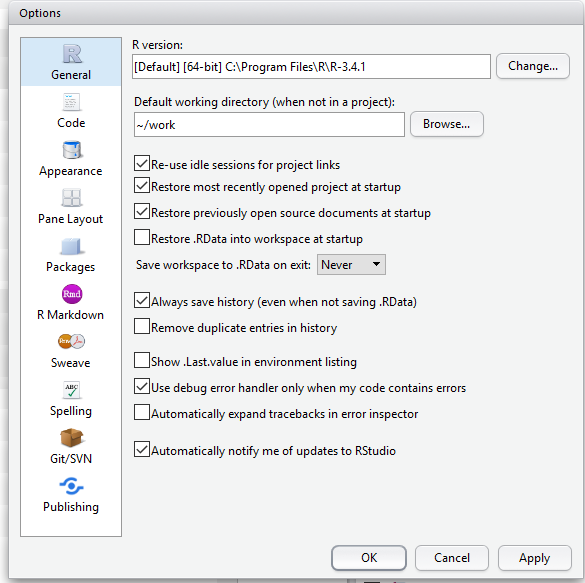
\includegraphics[width=1.95in,height=\textheight]{figs/rstudio-general.PNG}

次に, {[}Code{]} の タブ {[}Saving{]} で. {[}Default text encoding{]} を
\texttt{UTF-8} とする. Windows
以外だとOSのシステムフォントが同じなので問題ない. しかし Windows は SJIS
を拡張した CP932 なので, 注意が必要である.

Windows のRは UTF-8 を選択してもR自身はCP932処理している. ただ,
他のOSとの併用の場合, UTF-8 にしたほうがよいだろう. またHTMLファイルは
UTF-8 でのファイルが前提になりつつあるので, HTML
として出力を考えているなら, \texttt{UTF-8} としたほうが無難である.

またインターネットで公開されている日本語のRファイルは Windows
の使用が前提となっているため, 文字コードが CP932 であることが多い.
Windows 以外を使っている場合, 一時的に文字コードを SJIS
を選択する必要がある.

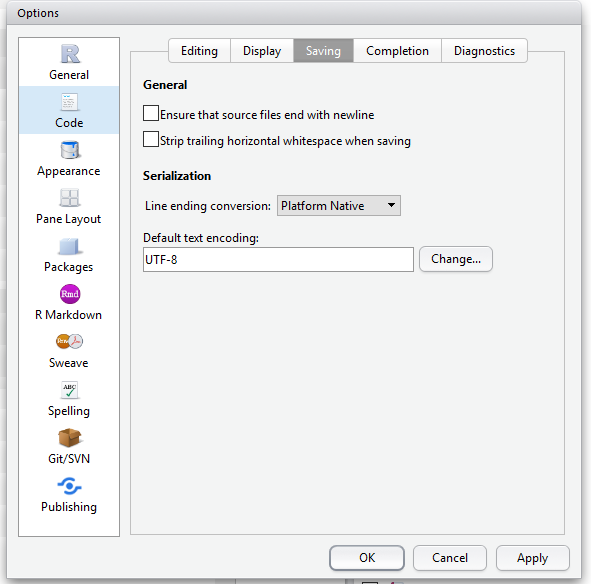
\includegraphics[width=1.97in,height=\textheight]{figs/rstudio-utf8.PNG}

あと, {[}R Markdown{]} で 真ん中あたりの {[}Show output preview in:{]}
を \texttt{View\ Pane} に変更する

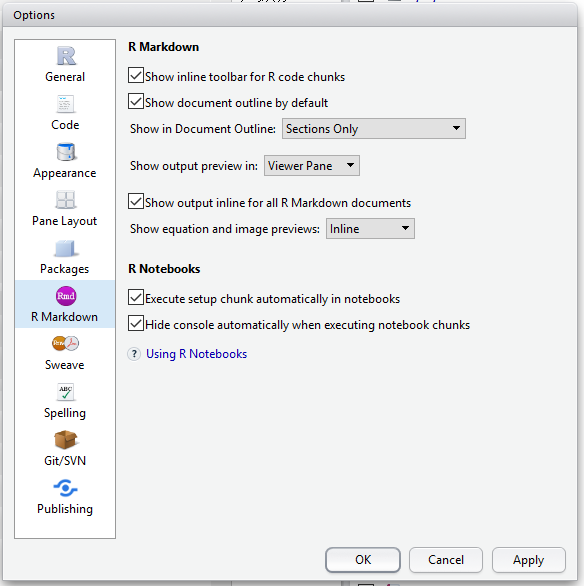
\includegraphics[width=1.95in,height=\textheight]{figs/rstudio-rmd.PNG}

\section{RStudio の使い方}\label{rstudio-ux306eux4f7fux3044ux65b9}

RStudio の使い方として日本語版のチートシートがある.

https://github.com/rstudio/cheatsheets/raw/master/translations/japanese/rstudio-IDE-cheatsheet\_ja.pdf

英語であるがこの動画も有益である. 第一章だけ公開されている.

https://www.datacamp.com/courses/working-with-the-rstudio-ide-part-1

RStudio
プロジェクト単位で複数のソースコードを管理するのことが推奨される.
そうするとプロジェクトごとに作業ディレクトリが設定される.
プロジェクトはメニューバー の {[}File{]} から {[}New Project{]}
を選択する. そうすると新たに新たにディレクトリを作成するか,
既存のディレクトリを採用するかなどが選べる. また,
バージョン管理ソフトを導入していればそこから取り入れることも可能となる.

\includegraphics{figs/rstudio_project.gif}

プロジェクトを立ち上げると左にコンソールペイン (Console Pane) が,
右側に上下に二分割されたペインが現れる. この配置は メニューバーの
{[}Tools{]} から {[}Project Options -\textgreater{} Pane Layout{]}
を選べば変更可能である.
コンソールペインにコマンドを入力するとその結果が直下に返される.
何か入力した後に, Ctrl + l (Cmd + l) を押すと, 画面が更新される.
上下の矢印キーで過去に実行したコマンドを選択できる.

メニューバー の {[}File{]} から {[}New File -\textgreater{} RScript{]}
を選択するか, Ctrl + Shift + n (Cmd + Shift + n) と入力するか,
メニューバー下の一番左の白紙のアイコンをクリックすると,
Rのスクリプトファイルが新規に作られる.
スクリプフォファイルを開くと左側のコンソール画面の上にソースペインが登場する.
ここにソースコードを書く.

ソースペインで何かコマンドを書いていきながら, ソースコードの該当行で
Ctrl + Enter (Cmd + Return) と入力するか,
ソースペインの上側の右に並んでいるアイコンのうち,
左側のRunと書かれたアイコンをクリックすると,
該当行がコンソール画面で実行される. 複数行選択した後に, メニューバー の
{[}Code{]} から {[}Run Selected line(s){]} を選ぶか, Ctrl + Shift +
Enter (Cmd + Shift + Enter)
と入力すると複数行をまとめて実行させることも可能である.

メニューバー の {[}File{]} から {[}Save{]} を選択するか, Ctrl + s (Cmd +
s) と入力するか,
メニューバー下の左から3番目のフロッピーディスクアイコンをクリック
すると, スクリプトファイルを保存することができる. またメニューバー の
{[}File{]} から {[}Open{]} を選択するか, Ctrl + o (Cmd + o)
と入力するか,
メニューバー下の左から2番めのフォルダを開くアイコンをクリックすると,
既存のスクリプトファイルを開くことができる.

\includegraphics{figs/rstudio_file.gif}

右上のペインには Environment と History のタブがある. Environment
は現在使っているオブジェクトが表示される. 最初は空白である.
変数に数値を代入 (R の言い方ではオブジェクトに付値) することによって,
値が付け加わっている. History はこれまでの履歴が記録される.
履歴の一部ををエディトペインかコンソールペインに挿入することができる.

右下のペインには Files, Plots, Packages, Help, Viewer のタブがある.
Files ペインはWindowsではエクスプローラーのようなもので, Mac はFinder
のようなもので, ファイル管理をおこなう.
ファイル管理として新たなフォルダを作成したり, ファイルを削除したり,
ファイル名を変更したりする.

またワーキングディレクトリを直感的に設定することもできる.
ワーキングを設定したい場所に移動して, Files
ペインの上に並んでいるアイコンのうち, Moreをクリックし, {[}Set As
Working Directory{]} をクリックすればよい.

Plots ペインはコンソール画面で作図をコマンドの実行したら,
表示されるペインである.
そこで作成した図をコマンドを使わずに保存したりすることができる. Packages
ペインは現在Rに導入されているパッケージリストが表示される.
そこに無いパッケージはメニューバーの {[}Tools{]} から {[}Install
Packages\ldots{]} を選択して実行すればよい. すでにあるパッケージは,
パッケージ名の左側のボックスをチェックすれば,
ライブライリ名を付けずにコマンドを実行させることができる.

Help ペインはその名の通り, ヘルプ画面が表示される. コンソールペインから
\texttt{help\ (コマンド)} もしくは \texttt{?コマンド}
と入力するとそのコマンドのヘルプがこのペインに表示される. R
ではソースペインやコンソールペインで, コマンド入力していると,
コマンドの後補があらわてくる. {[}TAB{]} でコマンドを補完できる.
さらにそのコマンドでどのような引数が使われるのかも示される. さらに
{[}TAB{]} を押せば, 引数を選べるだけでなく, 簡単なコマンドの説明がある.
そのときに {[}F1{]} を押せば, より詳細なヘルプが立ち上がる. また
Packages
パインから該当パッケージをクリックするとそのパッケージのコマンド一覧が
Help ペインに表示される.

\includegraphics{figs/rstudio_help.gif}

最後のViewer ペインは R Markdown で作成したファイルを
HTMLで出力したときに表示されるペインである.
最初の設定だと別のウィンドウ画面として結果が表示される.
このペインに出力されるためには {[}Tools -\textgreater{} R Markdown{]}
にいき, 真ん中あたりの {[}Show output preview in:{]} を View Pane
に変更する必要がある. その上でソースペインから {[}Ctrl + Shift + k{]}
とするか,
ソースペインの左側のアイコン群の一番右側のノートのアイコンをクリックすると,
確認画面が現れるので \texttt{HTML} を押す.
そうするとそのコードがすべて実行されて,
実行結果が作図も含めてHTMLファイルに出力される. もしくはメニューバーの
{[}File{]} から {[}Knit Document\ldots{]} としを選択するとよい.

\includegraphics{figs/rstudio_knit.gif}

これは knitr と rmarkdown いわれるパッケージを利用したもので,
Rのコードを埋め込んだマークダウンファイルを作成し,
そこからHTMLファイルを作成する. 他にも word ファイル や pdf
ファイル生成することも適切に設定していれば可能である.
ソースコードだけでなく, マークダウンファイルに \texttt{R}
コマンドを埋め込んだ \texttt{Rmd} ファイルを作成することができる
それは新規作成でRスクリプトでなく, R Notebook や R Markdown
を選択すればよい.

\bookmarksetup{startatroot}

\chapter{ベクトル}\label{ux30d9ux30afux30c8ux30eb}

\section{ベクトル}\label{ux30d9ux30afux30c8ux30eb-1}

R では同じ型の値を集めたものをベクトルという。 ベクトルは
\texttt{c()}(concatenate
の略)を用いて構成する。既存のベクトルを渡すと、ひと続きのベクトルとして結合される点にも注意する。

\begin{Shaded}
\begin{Highlighting}[]
\NormalTok{(num}\OtherTok{\textless{}{-}}\FunctionTok{c}\NormalTok{(}\DecValTok{2}\NormalTok{,}\DecValTok{3}\NormalTok{,}\DecValTok{7}\NormalTok{,}\DecValTok{9}\NormalTok{))}
\DocumentationTok{\#\# [1] 2 3 7 9}
\NormalTok{(chr }\OtherTok{\textless{}{-}} \FunctionTok{c}\NormalTok{(}\StringTok{"cat"}\NormalTok{,}\StringTok{"dog"}\NormalTok{,}\StringTok{"cow"}\NormalTok{))}
\DocumentationTok{\#\# [1] "cat" "dog" "cow"}
\end{Highlighting}
\end{Shaded}

ベクトルには長さという属性 (attribute) が付く。\texttt{length()}
で要素数を取得できるほか、\texttt{str()}
を使えばオブジェクトの構造をまとめて確認できる。

\begin{Shaded}
\begin{Highlighting}[]
\FunctionTok{length}\NormalTok{(num)}
\DocumentationTok{\#\# [1] 4}
\FunctionTok{length}\NormalTok{(chr)}
\DocumentationTok{\#\# [1] 3}
\end{Highlighting}
\end{Shaded}

ベクトルはオブジェクトの基本単位であり、単一の値も長さ 1
のベクトルとみなせる。

型が混在している場合は、自動的に最も表現力の高い型へ変換される。強制変換の優先順位は、おおむね「論理値
→ 数値 → 文字列」の順と覚えておくとよい。 文字列が 1
つでも含まれると、すべて文字列に変換される。
数値と論理値が混在している場合は、論理値が数値に強制変換され、\texttt{TRUE}
は 1、\texttt{FALSE} は 0 になる。

\begin{Shaded}
\begin{Highlighting}[]
\NormalTok{(x}\OtherTok{\textless{}{-}} \FunctionTok{c}\NormalTok{(}\DecValTok{1}\NormalTok{,}\DecValTok{4}\NormalTok{))}
\DocumentationTok{\#\# [1] 1 4}
\FunctionTok{typeof}\NormalTok{(x)}
\DocumentationTok{\#\# [1] "double"}
\NormalTok{(y }\OtherTok{\textless{}{-}} \FunctionTok{c}\NormalTok{(}\DecValTok{2}\NormalTok{,}\ConstantTok{FALSE}\NormalTok{,}\StringTok{"4"}\NormalTok{))}
\DocumentationTok{\#\# [1] "2"     "FALSE" "4"}
\FunctionTok{typeof}\NormalTok{(y)}
\DocumentationTok{\#\# [1] "character"}
\NormalTok{(z }\OtherTok{\textless{}{-}} \FunctionTok{c}\NormalTok{(}\DecValTok{2}\NormalTok{,}\ConstantTok{FALSE}\NormalTok{))}
\DocumentationTok{\#\# [1] 2 0}
\FunctionTok{typeof}\NormalTok{(z)}
\DocumentationTok{\#\# [1] "double"}
\end{Highlighting}
\end{Shaded}

\section{算術演算子}\label{ux7b97ux8853ux6f14ux7b97ux5b50}

四則演算などの算術演算子は要素ごとに適用される。\texttt{\^{}}
は累乗、\texttt{\%\%} は剰余、\texttt{\%/\%}
は整数除算(切り捨て)を表す。

\begin{Shaded}
\begin{Highlighting}[]
\NormalTok{a}\OtherTok{\textless{}{-}}\FunctionTok{c}\NormalTok{(}\DecValTok{2}\NormalTok{,}\DecValTok{3}\NormalTok{,}\DecValTok{3}\NormalTok{,}\DecValTok{3}\NormalTok{)}
\NormalTok{b}\OtherTok{\textless{}{-}}\FunctionTok{c}\NormalTok{(}\DecValTok{3}\NormalTok{,}\DecValTok{3}\NormalTok{,}\DecValTok{5}\NormalTok{,}\DecValTok{7}\NormalTok{)}
\NormalTok{a}\SpecialCharTok{+}\NormalTok{b}
\DocumentationTok{\#\# [1]  5  6  8 10}
\NormalTok{a}\SpecialCharTok{{-}}\NormalTok{b}
\DocumentationTok{\#\# [1] {-}1  0 {-}2 {-}4}
\NormalTok{a}\SpecialCharTok{*}\NormalTok{b}
\DocumentationTok{\#\# [1]  6  9 15 21}
\NormalTok{a}\SpecialCharTok{/}\NormalTok{b}
\DocumentationTok{\#\# [1] 0.6666667 1.0000000 0.6000000 0.4285714}
\NormalTok{a}\SpecialCharTok{\^{}}\NormalTok{b}
\DocumentationTok{\#\# [1]    8   27  243 2187}
\end{Highlighting}
\end{Shaded}

片方がスカラーであっても、同じ長さのベクトルに再利用されて演算される。

\begin{Shaded}
\begin{Highlighting}[]
\NormalTok{a}\SpecialCharTok{+}\DecValTok{2}
\DocumentationTok{\#\# [1] 4 5 5 5}
\NormalTok{a}\DecValTok{{-}2}
\DocumentationTok{\#\# [1] 0 1 1 1}
\NormalTok{a}\SpecialCharTok{*}\DecValTok{2}
\DocumentationTok{\#\# [1] 4 6 6 6}
\NormalTok{a}\SpecialCharTok{/}\DecValTok{2}
\DocumentationTok{\#\# [1] 1.0 1.5 1.5 1.5}
\NormalTok{a}\SpecialCharTok{\^{}}\DecValTok{2}
\DocumentationTok{\#\# [1] 4 9 9 9}
\end{Highlighting}
\end{Shaded}

長さが異なるベクトル同士を演算する場合、短い方のベクトルが自動的にリサイクルされて長さを揃える。

\begin{Shaded}
\begin{Highlighting}[]
\NormalTok{c}\OtherTok{\textless{}{-}}\FunctionTok{c}\NormalTok{(}\DecValTok{1}\NormalTok{,}\DecValTok{2}\NormalTok{)}
\NormalTok{a}\SpecialCharTok{+}\NormalTok{c}
\DocumentationTok{\#\# [1] 3 5 4 5}
\NormalTok{a}\SpecialCharTok{{-}}\NormalTok{c}
\DocumentationTok{\#\# [1] 1 1 2 1}
\NormalTok{a}\SpecialCharTok{*}\NormalTok{c}
\DocumentationTok{\#\# [1] 2 6 3 6}
\NormalTok{a}\SpecialCharTok{/}\NormalTok{c}
\DocumentationTok{\#\# [1] 2.0 1.5 3.0 1.5}
\NormalTok{a}\SpecialCharTok{\^{}}\NormalTok{c}
\DocumentationTok{\#\# [1] 2 9 3 9}
\end{Highlighting}
\end{Shaded}

ただし、短いベクトルの長さが長いベクトルの長さの約数でない場合は警告が表示される。

\section{論理演算子}\label{ux8ad6ux7406ux6f14ux7b97ux5b50}

論理値を入力に取り、論理値を返す演算子を論理演算子という。 R では、否定
(\texttt{!})、論理和 (\texttt{\textbar{}})、論理積 (\texttt{\&})
などの演算子が用意されている。 これらの演算子も要素ごとに評価される。
\texttt{\textbar{}\textbar{}} や \texttt{\&\&}
といった二重記号の演算子は、最初の要素のみを評価する短絡演算子であり、条件分岐で判定回数を抑えたいときに使う。

\begin{Shaded}
\begin{Highlighting}[]
\NormalTok{logic1 }\OtherTok{\textless{}{-}} \FunctionTok{c}\NormalTok{(}\ConstantTok{TRUE}\NormalTok{, }\ConstantTok{FALSE}\NormalTok{, }\ConstantTok{FALSE}\NormalTok{)}
\NormalTok{logic2 }\OtherTok{\textless{}{-}} \FunctionTok{c}\NormalTok{(}\ConstantTok{TRUE}\NormalTok{, }\ConstantTok{TRUE}\NormalTok{, }\ConstantTok{FALSE}\NormalTok{)}
\SpecialCharTok{!}\NormalTok{logic1}
\DocumentationTok{\#\# [1] FALSE  TRUE  TRUE}
\NormalTok{logic1 }\SpecialCharTok{|}\NormalTok{ logic2}
\DocumentationTok{\#\# [1]  TRUE  TRUE FALSE}
\NormalTok{logic1 }\SpecialCharTok{\&}\NormalTok{ logic2}
\DocumentationTok{\#\# [1]  TRUE FALSE FALSE}
\end{Highlighting}
\end{Shaded}

\texttt{all()} はすべての要素が \texttt{TRUE} かどうか、\texttt{any()}
は少なくとも 1 つが \texttt{TRUE} かどうかを判定する。

\begin{Shaded}
\begin{Highlighting}[]
\FunctionTok{any}\NormalTok{(logic1)}
\DocumentationTok{\#\# [1] TRUE}
\FunctionTok{all}\NormalTok{(logic1)}
\DocumentationTok{\#\# [1] FALSE}
\end{Highlighting}
\end{Shaded}

\section{比較演算子}\label{ux6bd4ux8f03ux6f14ux7b97ux5b50}

2 つの値を比較して論理値を返す演算子を比較演算子という。 R
では等しいかどうかを判定する \texttt{==}、大小を判定する
\texttt{\textgreater{}} や \texttt{\textless{}} などが用意されている。
これらもベクトルの要素ごとに評価される。

\begin{Shaded}
\begin{Highlighting}[]
\NormalTok{vec1 }\OtherTok{\textless{}{-}} \DecValTok{1}\SpecialCharTok{:}\DecValTok{4}
\NormalTok{vec2 }\OtherTok{\textless{}{-}} \FunctionTok{c}\NormalTok{(}\DecValTok{2}\NormalTok{,}\DecValTok{1}\NormalTok{,}\DecValTok{3}\NormalTok{,}\DecValTok{4}\NormalTok{)}
\NormalTok{vec1 }\SpecialCharTok{==}\NormalTok{ vec2}
\DocumentationTok{\#\# [1] FALSE FALSE  TRUE  TRUE}
\NormalTok{vec1 }\SpecialCharTok{\textgreater{}}\NormalTok{ vec2}
\DocumentationTok{\#\# [1] FALSE  TRUE FALSE FALSE}
\NormalTok{vec1 }\SpecialCharTok{\textless{}}\NormalTok{ vec2}
\DocumentationTok{\#\# [1]  TRUE FALSE FALSE FALSE}
\end{Highlighting}
\end{Shaded}

不等号として
\texttt{!=}(等しくない)、\texttt{\textgreater{}=}(以上)、\texttt{\textless{}=}(以下)も利用できる。

\begin{Shaded}
\begin{Highlighting}[]
\NormalTok{vec1 }\SpecialCharTok{!=}\NormalTok{ vec2 }\CommentTok{\# !(vec1==vec2)}
\DocumentationTok{\#\# [1]  TRUE  TRUE FALSE FALSE}
\NormalTok{vec1 }\SpecialCharTok{\textgreater{}=}\NormalTok{ vec2 }\CommentTok{\# (vec1 \textgreater{} vec2 | vec1 == vec2)}
\DocumentationTok{\#\# [1] FALSE  TRUE  TRUE  TRUE}
\NormalTok{vec1 }\SpecialCharTok{\textless{}=}\NormalTok{ vec2 }\CommentTok{\# (vec1 \textless{} vec2 | vec1 == vec2)}
\DocumentationTok{\#\# [1]  TRUE FALSE  TRUE  TRUE}
\end{Highlighting}
\end{Shaded}

スカラーとベクトルを比較する場合は、スカラーが再利用されて要素ごとに評価される。

\begin{Shaded}
\begin{Highlighting}[]
\NormalTok{vec1 }\SpecialCharTok{\textgreater{}} \DecValTok{2}
\DocumentationTok{\#\# [1] FALSE FALSE  TRUE  TRUE}
\end{Highlighting}
\end{Shaded}

\texttt{\%in\%}
演算子を使うと、左側のベクトル要素が右側のベクトルに含まれているかを判定できる。返り値は論理値のベクトルで、元の長さと同じになる。

\begin{Shaded}
\begin{Highlighting}[]
\NormalTok{vec1 }\SpecialCharTok{\%in\%} \DecValTok{4}\SpecialCharTok{:}\DecValTok{5}
\DocumentationTok{\#\# [1] FALSE FALSE FALSE  TRUE}
\end{Highlighting}
\end{Shaded}

\section{要素}\label{ux8981ux7d20}

ベクトルの要素は角括弧で取り出す。

\begin{Shaded}
\begin{Highlighting}[]
\NormalTok{num }\OtherTok{\textless{}{-}} \FunctionTok{c}\NormalTok{(}\DecValTok{2}\NormalTok{,}\DecValTok{3}\NormalTok{,}\DecValTok{7}\NormalTok{,}\DecValTok{9}\NormalTok{)}
\NormalTok{num[}\DecValTok{3}\NormalTok{]}
\DocumentationTok{\#\# [1] 7}
\end{Highlighting}
\end{Shaded}

取り出すだけでなく、新しい値を代入することもできる。

\begin{Shaded}
\begin{Highlighting}[]
\NormalTok{num[}\DecValTok{3}\NormalTok{] }\OtherTok{\textless{}{-}} \DecValTok{500}
\NormalTok{num}
\DocumentationTok{\#\# [1]   2   3 500   9}
\end{Highlighting}
\end{Shaded}

負のインデックスを指定すると、その位置の要素を除いたベクトルが得られる。

\begin{Shaded}
\begin{Highlighting}[]
\NormalTok{num[}\SpecialCharTok{{-}}\DecValTok{3}\NormalTok{]}
\DocumentationTok{\#\# [1] 2 3 9}
\end{Highlighting}
\end{Shaded}

複数の要素を同時に取り出すことも容易である。

\begin{Shaded}
\begin{Highlighting}[]
\NormalTok{num[}\FunctionTok{c}\NormalTok{(}\DecValTok{1}\NormalTok{,}\DecValTok{4}\NormalTok{)]}
\DocumentationTok{\#\# [1] 2 9}
\end{Highlighting}
\end{Shaded}

論理値ベクトルをインデックスとして使えば、条件に合致する要素のみを抽出できる。

\begin{Shaded}
\begin{Highlighting}[]
\NormalTok{idx }\OtherTok{\textless{}{-}} \FunctionTok{c}\NormalTok{(}\ConstantTok{TRUE}\NormalTok{,}\ConstantTok{FALSE}\NormalTok{,}\ConstantTok{TRUE}\NormalTok{,}\ConstantTok{TRUE}\NormalTok{)}
\NormalTok{num[idx]}
\DocumentationTok{\#\# [1]   2 500   9}
\end{Highlighting}
\end{Shaded}

比較演算子と組み合わせれば、条件式を直接インデックスに渡してフィルタリングできる。

\begin{Shaded}
\begin{Highlighting}[]
\NormalTok{(num }\SpecialCharTok{\textgreater{}} \DecValTok{4}\NormalTok{)}
\DocumentationTok{\#\# [1] FALSE FALSE  TRUE  TRUE}
\NormalTok{num[num }\SpecialCharTok{\textgreater{}} \DecValTok{4}\NormalTok{]}
\DocumentationTok{\#\# [1] 500   9}
\end{Highlighting}
\end{Shaded}

\texttt{:}
演算子で連続した整数ベクトルを生成し、その範囲を指定して抜き出すこともできる。非整数のステップや逆順が必要な場合は
\texttt{seq()} を利用すると柔軟に制御できる。

\begin{Shaded}
\begin{Highlighting}[]
\DecValTok{2}\SpecialCharTok{:}\DecValTok{4}
\DocumentationTok{\#\# [1] 2 3 4}
\NormalTok{num[}\DecValTok{2}\SpecialCharTok{:}\DecValTok{4}\NormalTok{]}
\DocumentationTok{\#\# [1]   3 500   9}
\end{Highlighting}
\end{Shaded}

ベクトルには名前属性を付与できる。

\begin{Shaded}
\begin{Highlighting}[]
\NormalTok{vec }\OtherTok{\textless{}{-}} \FunctionTok{c}\NormalTok{(}\AttributeTok{x=} \DecValTok{3}\NormalTok{, }\AttributeTok{y =}\DecValTok{3}\NormalTok{, }\AttributeTok{z =} \DecValTok{4}\NormalTok{)}
\end{Highlighting}
\end{Shaded}

別の方法として次のように設定できる。

\begin{Shaded}
\begin{Highlighting}[]
\FunctionTok{names}\NormalTok{(num) }\OtherTok{\textless{}{-}}\NormalTok{ letters[}\DecValTok{1}\SpecialCharTok{:}\DecValTok{4}\NormalTok{]}
\end{Highlighting}
\end{Shaded}

名前を付けると、文字列で要素を参照できる。

\begin{Shaded}
\begin{Highlighting}[]
\NormalTok{vec[}\StringTok{"x"}\NormalTok{]}
\DocumentationTok{\#\# x }
\DocumentationTok{\#\# 3}
\NormalTok{num[}\StringTok{"d"}\NormalTok{]}
\DocumentationTok{\#\# d }
\DocumentationTok{\#\# 9}
\end{Highlighting}
\end{Shaded}

現在の名前一覧は \texttt{names()} で取得でき、不要になった場合は
\texttt{names(num)\ \textless{}-\ NULL} のようにして削除する。

\section{関数}\label{ux95a2ux6570}

ベクトルを引数に取る関数も多数用意されており、和や積などを簡単に計算できる。累積和(\texttt{cumsum()})や累積積(\texttt{cumprod()})は系列データの推移を追跡したいときに便利である。

\begin{Shaded}
\begin{Highlighting}[]
\NormalTok{x}\OtherTok{\textless{}{-}}\FunctionTok{c}\NormalTok{(}\DecValTok{1}\NormalTok{,}\DecValTok{2}\NormalTok{,}\DecValTok{3}\NormalTok{,}\DecValTok{4}\NormalTok{,}\DecValTok{5}\NormalTok{)}
\FunctionTok{sum}\NormalTok{(x)}
\DocumentationTok{\#\# [1] 15}
\FunctionTok{cumsum}\NormalTok{(x)}
\DocumentationTok{\#\# [1]  1  3  6 10 15}
\FunctionTok{prod}\NormalTok{(x)}
\DocumentationTok{\#\# [1] 120}
\FunctionTok{cumprod}\NormalTok{(x)}
\DocumentationTok{\#\# [1]   1   2   6  24 120}
\end{Highlighting}
\end{Shaded}

平均、中央値、分散、標準偏差といった統計量もワンライナーで求められる。

\begin{Shaded}
\begin{Highlighting}[]
\NormalTok{x }\OtherTok{\textless{}{-}} \FunctionTok{c}\NormalTok{(x,}\DecValTok{10}\NormalTok{)}
\FunctionTok{mean}\NormalTok{(x)}
\DocumentationTok{\#\# [1] 4.166667}
\FunctionTok{median}\NormalTok{(x)}
\DocumentationTok{\#\# [1] 3.5}
\FunctionTok{var}\NormalTok{(x)}
\DocumentationTok{\#\# [1] 10.16667}
\FunctionTok{sd}\NormalTok{(x)}
\DocumentationTok{\#\# [1] 3.188521}
\end{Highlighting}
\end{Shaded}

ベクトルを並べ替えたり、最小値・最大値やその位置を取得したりする関数も充実している。

\begin{Shaded}
\begin{Highlighting}[]
\NormalTok{x }\OtherTok{\textless{}{-}} \FunctionTok{c}\NormalTok{(}\DecValTok{3}\NormalTok{,}\DecValTok{3}\NormalTok{,}\DecValTok{5}\NormalTok{,}\DecValTok{0}\NormalTok{)}
\FunctionTok{sort}\NormalTok{(x)}
\DocumentationTok{\#\# [1] 0 3 3 5}
\FunctionTok{sort}\NormalTok{(x,}\AttributeTok{decreasing =} \ConstantTok{TRUE}\NormalTok{)}
\DocumentationTok{\#\# [1] 5 3 3 0}
\FunctionTok{min}\NormalTok{(x)}
\DocumentationTok{\#\# [1] 0}
\FunctionTok{max}\NormalTok{(x)}
\DocumentationTok{\#\# [1] 5}
\FunctionTok{which.min}\NormalTok{(x)}
\DocumentationTok{\#\# [1] 4}
\FunctionTok{which.max}\NormalTok{(x)}
\DocumentationTok{\#\# [1] 3}
\end{Highlighting}
\end{Shaded}

欠損値 \texttt{NA} が含まれている場合、\texttt{mean()}
など多くの集計関数は既定の挙動として \texttt{NA} を返す。
集計から欠損を除外したいときは、\texttt{na.rm\ =\ TRUE} を指定する。

\begin{Shaded}
\begin{Highlighting}[]
\NormalTok{x }\OtherTok{\textless{}{-}} \FunctionTok{c}\NormalTok{(}\DecValTok{4}\NormalTok{,}\DecValTok{2}\NormalTok{,}\ConstantTok{NA}\NormalTok{,}\DecValTok{3}\NormalTok{)}
\FunctionTok{mean}\NormalTok{(x)}
\DocumentationTok{\#\# [1] NA}
\FunctionTok{mean}\NormalTok{(x, }\AttributeTok{na.rm =} \ConstantTok{TRUE}\NormalTok{)}
\DocumentationTok{\#\# [1] 3}
\end{Highlighting}
\end{Shaded}

\section{規則的なベクトル}\label{ux898fux5247ux7684ux306aux30d9ux30afux30c8ux30eb}

\texttt{1:5} のような規則的なベクトルを柔軟に作成するのに \texttt{seq}
を用いるとよい。

\begin{Shaded}
\begin{Highlighting}[]
\DecValTok{1}\SpecialCharTok{:}\DecValTok{5}
\DocumentationTok{\#\# [1] 1 2 3 4 5}
\FunctionTok{seq}\NormalTok{(}\DecValTok{1}\NormalTok{, }\DecValTok{5}\NormalTok{)}
\DocumentationTok{\#\# [1] 1 2 3 4 5}
\FunctionTok{seq}\NormalTok{(}\DecValTok{1}\NormalTok{, }\DecValTok{5}\NormalTok{, }\AttributeTok{by =} \DecValTok{2}\NormalTok{)}
\DocumentationTok{\#\# [1] 1 3 5}
\FunctionTok{seq}\NormalTok{(}\DecValTok{1}\NormalTok{, }\DecValTok{5}\NormalTok{, }\AttributeTok{length.out =} \DecValTok{4}\NormalTok{)}
\DocumentationTok{\#\# [1] 1.000000 2.333333 3.666667 5.000000}
\end{Highlighting}
\end{Shaded}

繰り返しを作成することができる \texttt{rep} も覚えておくと便利である。

\begin{Shaded}
\begin{Highlighting}[]
\FunctionTok{rep}\NormalTok{(}\DecValTok{1}\NormalTok{, }\DecValTok{5}\NormalTok{)}
\DocumentationTok{\#\# [1] 1 1 1 1 1}
\FunctionTok{rep}\NormalTok{(}\FunctionTok{c}\NormalTok{(}\DecValTok{1}\NormalTok{, }\DecValTok{2}\NormalTok{), }\AttributeTok{times =} \DecValTok{3}\NormalTok{)}
\DocumentationTok{\#\# [1] 1 2 1 2 1 2}
\FunctionTok{rep}\NormalTok{(}\FunctionTok{c}\NormalTok{(}\DecValTok{1}\NormalTok{, }\DecValTok{2}\NormalTok{), }\AttributeTok{each =} \DecValTok{3}\NormalTok{)}
\DocumentationTok{\#\# [1] 1 1 1 2 2 2}
\end{Highlighting}
\end{Shaded}

またアルファベットの文字列もあらかじめ組み込まれている。

\begin{Shaded}
\begin{Highlighting}[]
\NormalTok{letters}
\DocumentationTok{\#\#  [1] "a" "b" "c" "d" "e" "f" "g" "h" "i" "j" "k" "l" "m" "n" "o" "p" "q" "r" "s"}
\DocumentationTok{\#\# [20] "t" "u" "v" "w" "x" "y" "z"}
\NormalTok{LETTERS}
\DocumentationTok{\#\#  [1] "A" "B" "C" "D" "E" "F" "G" "H" "I" "J" "K" "L" "M" "N" "O" "P" "Q" "R" "S"}
\DocumentationTok{\#\# [20] "T" "U" "V" "W" "X" "Y" "Z"}
\NormalTok{LETTERS[}\DecValTok{1}\SpecialCharTok{:}\DecValTok{2}\NormalTok{]}
\DocumentationTok{\#\# [1] "A" "B"}
\end{Highlighting}
\end{Shaded}

\section{乱数ベクトル}\label{ux4e71ux6570ux30d9ux30afux30c8ux30eb}

ベクトルを無作為に並べ替えたり抽出したりするには \texttt{sample()}
を使う。

\begin{Shaded}
\begin{Highlighting}[]
\FunctionTok{set.seed}\NormalTok{(}\DecValTok{10}\NormalTok{)}
\FunctionTok{sample}\NormalTok{(}\DecValTok{1}\SpecialCharTok{:}\DecValTok{5}\NormalTok{)}
\DocumentationTok{\#\# [1] 3 1 2 5 4}
\end{Highlighting}
\end{Shaded}

ここで \texttt{set.seed()}
は乱数の種を固定し、別の環境でも同じ結果を再現できるようにするための設定である。

上記は一度選ばれた値を再度選ばない非復元抽出である。復元抽出にする場合は
\texttt{replace\ =\ TRUE} を指定する。

\begin{Shaded}
\begin{Highlighting}[]
\FunctionTok{sample}\NormalTok{(}\DecValTok{1}\SpecialCharTok{:}\DecValTok{5}\NormalTok{, }\AttributeTok{replace =} \ConstantTok{TRUE}\NormalTok{)}
\DocumentationTok{\#\# [1] 3 2 2 2 5}
\end{Highlighting}
\end{Shaded}

\texttt{size} 引数を指定すれば、取り出す要素数も制御できる。

\begin{Shaded}
\begin{Highlighting}[]
\FunctionTok{sample}\NormalTok{(LETTERS[}\DecValTok{1}\SpecialCharTok{:}\DecValTok{2}\NormalTok{], }\AttributeTok{size =} \DecValTok{10}\NormalTok{, }\AttributeTok{replace =} \ConstantTok{TRUE}\NormalTok{)}
\DocumentationTok{\#\#  [1] "A" "B" "B" "A" "B" "A" "A" "B" "B" "A"}
\end{Highlighting}
\end{Shaded}

非復元抽出では、\texttt{size}
を母集合の長さより大きくすることはできない点に注意する。

さらに \texttt{prob} で各要素が選ばれる確率を指定できる(確率の合計は 1
になるようにする)。

\begin{Shaded}
\begin{Highlighting}[]
\FunctionTok{sample}\NormalTok{(LETTERS[}\DecValTok{1}\SpecialCharTok{:}\DecValTok{2}\NormalTok{], }\AttributeTok{prob =} \FunctionTok{c}\NormalTok{(}\FloatTok{0.8}\NormalTok{, }\FloatTok{0.2}\NormalTok{), }\AttributeTok{size =} \DecValTok{10}\NormalTok{, }\AttributeTok{replace =} \ConstantTok{TRUE}\NormalTok{)}
\DocumentationTok{\#\#  [1] "A" "A" "A" "B" "A" "A" "B" "B" "A" "A"}
\end{Highlighting}
\end{Shaded}

独立な一様分布に従う長さ \texttt{size} のベクトルは
\texttt{runif(size)}、平均と分散を指定した正規分布なら
\texttt{rnorm(size,\ mean,\ sd)} で生成できる(既定値は平均 0、標準偏差
1)。

\begin{Shaded}
\begin{Highlighting}[]
\NormalTok{size }\OtherTok{\textless{}{-}} \DecValTok{8}
\FunctionTok{runif}\NormalTok{(size)}
\DocumentationTok{\#\# [1] 0.27548386 0.22890394 0.01443391 0.72896456 0.24988047 0.16118328 0.01704265}
\DocumentationTok{\#\# [8] 0.48610035}
\FunctionTok{rnorm}\NormalTok{(size)}
\DocumentationTok{\#\# [1] {-}1.26519802 {-}0.37366156 {-}0.68755543 {-}0.87215883 {-}0.10176101 {-}0.25378053}
\DocumentationTok{\#\# [7] {-}1.85374045 {-}0.07794607}
\end{Highlighting}
\end{Shaded}

\bookmarksetup{startatroot}

\chapter{データ構造}\label{ux30c7ux30fcux30bfux69cbux9020}

\section{リスト}\label{ux30eaux30b9ux30c8}

複数のオブジェクト(ベクトルや別のリストなど)をまとめたものがリストである。
型の異なるベクトルでも \texttt{list()} に渡すことで 1
つのリストにまとめられる。

リストにも長さという属性があり、\texttt{length()} で要素数を確認できる。

\begin{Shaded}
\begin{Highlighting}[]
\NormalTok{(lst }\OtherTok{\textless{}{-}} \FunctionTok{list}\NormalTok{(}\StringTok{"a"}\NormalTok{,}\FunctionTok{c}\NormalTok{(}\DecValTok{3}\NormalTok{,}\DecValTok{3}\NormalTok{,}\DecValTok{2}\NormalTok{)))}
\DocumentationTok{\#\# [[1]]}
\DocumentationTok{\#\# [1] "a"}
\DocumentationTok{\#\# }
\DocumentationTok{\#\# [[2]]}
\DocumentationTok{\#\# [1] 3 3 2}
\FunctionTok{typeof}\NormalTok{(lst)}
\DocumentationTok{\#\# [1] "list"}
\FunctionTok{length}\NormalTok{(lst)}
\DocumentationTok{\#\# [1] 2}
\end{Highlighting}
\end{Shaded}

\texttt{class()} でオブジェクトのクラスを、\texttt{str()}
で内部構造を確認できる。

\begin{Shaded}
\begin{Highlighting}[]
\FunctionTok{class}\NormalTok{(lst)}
\DocumentationTok{\#\# [1] "list"}
\FunctionTok{str}\NormalTok{(lst)}
\DocumentationTok{\#\# List of 2}
\DocumentationTok{\#\#  $ : chr "a"}
\DocumentationTok{\#\#  $ : num [1:3] 3 3 2}
\end{Highlighting}
\end{Shaded}

リストは入れ子にすることもできる。これは単一の型しか持てないベクトルとの大きな違いである。

\begin{Shaded}
\begin{Highlighting}[]
\FunctionTok{typeof}\NormalTok{(}\FunctionTok{list}\NormalTok{(}\StringTok{"b"}\NormalTok{,lst))}
\DocumentationTok{\#\# [1] "list"}
\end{Highlighting}
\end{Shaded}

リストをベクトルに変換するには \texttt{unlist()}
を使う。構成要素の型が異なる場合は、ベクトルに変換できるように強制変換が行われる。

\begin{Shaded}
\begin{Highlighting}[]
\NormalTok{lst}\OtherTok{\textless{}{-}}\FunctionTok{list}\NormalTok{(}\DecValTok{1}\SpecialCharTok{:}\DecValTok{3}\NormalTok{,}\DecValTok{2}\SpecialCharTok{:}\DecValTok{6}\NormalTok{)}
\NormalTok{lst}
\DocumentationTok{\#\# [[1]]}
\DocumentationTok{\#\# [1] 1 2 3}
\DocumentationTok{\#\# }
\DocumentationTok{\#\# [[2]]}
\DocumentationTok{\#\# [1] 2 3 4 5 6}
\FunctionTok{unlist}\NormalTok{(lst)}
\DocumentationTok{\#\# [1] 1 2 3 2 3 4 5 6}
\FunctionTok{unlist}\NormalTok{(}\FunctionTok{list}\NormalTok{(}\StringTok{"a"}\NormalTok{,}\DecValTok{1}\SpecialCharTok{:}\DecValTok{4}\NormalTok{))}
\DocumentationTok{\#\# [1] "a" "1" "2" "3" "4"}
\end{Highlighting}
\end{Shaded}

個々の要素の長さを調べたいときは \texttt{lengths(lst)}
が便利で、各要素に同じ処理を施す場合は \texttt{lapply()} や
\texttt{sapply()} を組み合わせるとよい。

\subsection{リストのアクセス}\label{ux30eaux30b9ux30c8ux306eux30a2ux30afux30bbux30b9}

リストの要素も角括弧を用いて参照する。単一の角括弧 \texttt{{[}{]}}
を使うと、要素を取り出してもリストのまま返る。以下は最初の要素(= 1
番目のリスト)を取得する例である。

\begin{Shaded}
\begin{Highlighting}[]
\NormalTok{lst[}\DecValTok{1}\NormalTok{]}
\DocumentationTok{\#\# [[1]]}
\DocumentationTok{\#\# [1] 1 2 3}
\end{Highlighting}
\end{Shaded}

名前属性を付けたリストであれば、文字列でアクセスできる。

\begin{Shaded}
\begin{Highlighting}[]
\NormalTok{(lst }\OtherTok{\textless{}{-}} \FunctionTok{list}\NormalTok{(}\AttributeTok{name=}\StringTok{"a"}\NormalTok{,}\AttributeTok{num=}\FunctionTok{c}\NormalTok{(}\DecValTok{3}\NormalTok{,}\DecValTok{3}\NormalTok{,}\DecValTok{2}\NormalTok{)))}
\DocumentationTok{\#\# $name}
\DocumentationTok{\#\# [1] "a"}
\DocumentationTok{\#\# }
\DocumentationTok{\#\# $num}
\DocumentationTok{\#\# [1] 3 3 2}
\FunctionTok{names}\NormalTok{(lst)}
\DocumentationTok{\#\# [1] "name" "num"}
\end{Highlighting}
\end{Shaded}

この状態で次のように書けば 2 番目の要素を取り出せる。

\begin{Shaded}
\begin{Highlighting}[]
\NormalTok{lst[}\StringTok{"num"}\NormalTok{]}
\DocumentationTok{\#\# $num}
\DocumentationTok{\#\# [1] 3 3 2}
\end{Highlighting}
\end{Shaded}

いずれの場合も \texttt{{[}{]}}
で取り出した結果はリストである点に注意する。

\begin{Shaded}
\begin{Highlighting}[]
\FunctionTok{typeof}\NormalTok{(lst[}\DecValTok{1}\NormalTok{])}
\DocumentationTok{\#\# [1] "list"}
\FunctionTok{typeof}\NormalTok{(lst[}\StringTok{"num"}\NormalTok{])}
\DocumentationTok{\#\# [1] "list"}
\end{Highlighting}
\end{Shaded}

ベクトルとして取り出したい場合は二重角括弧 \texttt{{[}{[}\ {]}{]}}
を使う。これによりリスト要素の中身がそのまま返る。

\begin{Shaded}
\begin{Highlighting}[]
\NormalTok{lst[[}\DecValTok{2}\NormalTok{]]}
\DocumentationTok{\#\# [1] 3 3 2}
\FunctionTok{typeof}\NormalTok{(lst[[}\DecValTok{2}\NormalTok{]])}
\DocumentationTok{\#\# [1] "double"}
\end{Highlighting}
\end{Shaded}

名前付きの場合は次のように書くこともできる。

\begin{Shaded}
\begin{Highlighting}[]
\NormalTok{lst[[}\StringTok{"num"}\NormalTok{]]}
\DocumentationTok{\#\# [1] 3 3 2}
\NormalTok{lst}\SpecialCharTok{$}\NormalTok{num}
\DocumentationTok{\#\# [1] 3 3 2}
\end{Highlighting}
\end{Shaded}

リスト内のベクトルに対して関数を適用したいときは、二重括弧か \texttt{\$}
記法でベクトルを取り出してから利用する。次の例では \texttt{\$}
記法を使っているが、コメント行で示したように二重括弧を使っても結果は同じである。

\begin{Shaded}
\begin{Highlighting}[]
\DocumentationTok{\#\# mean(lst[[2]])}
\DocumentationTok{\#\# mean(lst[["num"]])}
\FunctionTok{mean}\NormalTok{(lst}\SpecialCharTok{$}\NormalTok{num)}
\DocumentationTok{\#\# [1] 2.666667}
\end{Highlighting}
\end{Shaded}

\texttt{with()} を使えば、リスト内の要素を名前だけで参照できる。

\begin{Shaded}
\begin{Highlighting}[]
\FunctionTok{with}\NormalTok{(lst, }\FunctionTok{mean}\NormalTok{(num))}
\DocumentationTok{\#\# [1] 2.666667}
\end{Highlighting}
\end{Shaded}

リストの要素を削除したいときは、該当要素に \texttt{NULL} を代入する。

\begin{Shaded}
\begin{Highlighting}[]
\NormalTok{lst}\SpecialCharTok{$}\NormalTok{num }\OtherTok{\textless{}{-}} \ConstantTok{NULL}
\NormalTok{lst}
\DocumentationTok{\#\# $name}
\DocumentationTok{\#\# [1] "a"}
\end{Highlighting}
\end{Shaded}

\section{因子ベクトル}\label{ux56e0ux5b50ux30d9ux30afux30c8ux30eb}

\subsection{factor}\label{factor}

文字列ベクトルを \texttt{factor()} に渡すと、カテゴリ情報を持つ因子
(factor) ベクトルを作成できる。

\begin{Shaded}
\begin{Highlighting}[]
\NormalTok{(x }\OtherTok{\textless{}{-}} \FunctionTok{c}\NormalTok{(}\StringTok{"L"}\NormalTok{,}\StringTok{"S"}\NormalTok{,}\StringTok{"M"}\NormalTok{,}\StringTok{"M"}\NormalTok{,}\StringTok{"L"}\NormalTok{))}
\DocumentationTok{\#\# [1] "L" "S" "M" "M" "L"}
\NormalTok{(x.fac }\OtherTok{\textless{}{-}} \FunctionTok{factor}\NormalTok{(x))}
\DocumentationTok{\#\# [1] L S M M L}
\DocumentationTok{\#\# Levels: L M S}
\end{Highlighting}
\end{Shaded}

因子ベクトルの実体は、\texttt{levels}
という属性を持つ整数ベクトルである。値そのものではなく水準の位置を保持している点に注意する。

\begin{Shaded}
\begin{Highlighting}[]
\FunctionTok{typeof}\NormalTok{(x.fac)}
\DocumentationTok{\#\# [1] "integer"}
\FunctionTok{length}\NormalTok{(x.fac)}
\DocumentationTok{\#\# [1] 5}
\FunctionTok{levels}\NormalTok{(x.fac)}
\DocumentationTok{\#\# [1] "L" "M" "S"}
\end{Highlighting}
\end{Shaded}

\texttt{class()} で因子であることを確認し、\texttt{str()}
で水準情報などの属性を詳しく確認できる。

\begin{Shaded}
\begin{Highlighting}[]
\FunctionTok{class}\NormalTok{(x.fac)}
\DocumentationTok{\#\# [1] "factor"}
\FunctionTok{str}\NormalTok{(x.fac)}
\DocumentationTok{\#\#  Factor w/ 3 levels "L","M","S": 1 3 2 2 1}
\end{Highlighting}
\end{Shaded}

水準の表示順は既定ではアルファベット順に並ぶが、\texttt{levels}
引数を指定すれば任意の順に設定できる。

\begin{Shaded}
\begin{Highlighting}[]
\NormalTok{(x.factor }\OtherTok{\textless{}{-}} \FunctionTok{factor}\NormalTok{(x,}\AttributeTok{levels=}\FunctionTok{c}\NormalTok{(}\StringTok{"S"}\NormalTok{,}\StringTok{"M"}\NormalTok{,}\StringTok{"L"}\NormalTok{)))}
\DocumentationTok{\#\# [1] L S M M L}
\DocumentationTok{\#\# Levels: S M L}
\end{Highlighting}
\end{Shaded}

さらに \texttt{ordered()}
を使うと、水準に大小関係(順序)を持たせた因子を作れる。

\begin{Shaded}
\begin{Highlighting}[]
\NormalTok{(x.order }\OtherTok{\textless{}{-}} \FunctionTok{ordered}\NormalTok{(x,}\AttributeTok{levels=}\FunctionTok{c}\NormalTok{(}\StringTok{"S"}\NormalTok{,}\StringTok{"M"}\NormalTok{,}\StringTok{"L"}\NormalTok{)))}
\DocumentationTok{\#\# [1] L S M M L}
\DocumentationTok{\#\# Levels: S \textless{} M \textless{} L}
\end{Highlighting}
\end{Shaded}

分析の途中で未使用の水準を落としたいときは \texttt{droplevels(x.factor)}
を利用する。

\subsection{cut}\label{cut}

連続値を区間ごとに区分して因子化したい場合は \texttt{cut()}
を用いる。まず 0 から 10 までの値を乱数で生成する。

\begin{Shaded}
\begin{Highlighting}[]
\NormalTok{x }\OtherTok{\textless{}{-}} \FunctionTok{runif}\NormalTok{(}\DecValTok{10}\NormalTok{,}\DecValTok{0}\NormalTok{,}\DecValTok{10}\NormalTok{)}
\NormalTok{x}
\DocumentationTok{\#\#  [1] 4.2637965 2.0204400 7.7383107 8.1929405 3.1325967 0.8670448 6.6741102}
\DocumentationTok{\#\#  [8] 3.8639900 3.9642807 1.0927404}
\end{Highlighting}
\end{Shaded}

\texttt{breaks}
に分割数を指定すると、最小値から最大値までを等間隔に区切る。

\begin{Shaded}
\begin{Highlighting}[]
\FunctionTok{cut}\NormalTok{(x, }\AttributeTok{breaks=}\DecValTok{5}\NormalTok{)}
\DocumentationTok{\#\#  [1] (3.8,5.26]  (0.86,2.33] (6.73,8.2]  (6.73,8.2]  (2.33,3.8]  (0.86,2.33]}
\DocumentationTok{\#\#  [7] (5.26,6.73] (3.8,5.26]  (3.8,5.26]  (0.86,2.33]}
\DocumentationTok{\#\# Levels: (0.86,2.33] (2.33,3.8] (3.8,5.26] (5.26,6.73] (6.73,8.2]}
\end{Highlighting}
\end{Shaded}

これは観測値の最小値から最大値までの区間を 5 等分した結果を返している。

区間境界を自分で指定したい場合は、\texttt{breaks} に数値ベクトルを渡す。

\begin{Shaded}
\begin{Highlighting}[]
\FunctionTok{cut}\NormalTok{(x,}\AttributeTok{breaks=}\FunctionTok{c}\NormalTok{(}\DecValTok{0}\NormalTok{,}\DecValTok{2}\NormalTok{,}\DecValTok{4}\NormalTok{,}\DecValTok{6}\NormalTok{,}\DecValTok{8}\NormalTok{,}\DecValTok{10}\NormalTok{))}
\DocumentationTok{\#\#  [1] (4,6]  (2,4]  (6,8]  (8,10] (2,4]  (0,2]  (6,8]  (2,4]  (2,4]  (0,2] }
\DocumentationTok{\#\# Levels: (0,2] (2,4] (4,6] (6,8] (8,10]}
\end{Highlighting}
\end{Shaded}

0 より大きく 2 以下、2 より大きく 4 以下、\ldots{}
のように区切られている。

最初の区間に最小値を含めたいときは \texttt{include.lowest\ =\ TRUE}
を指定する。

\begin{Shaded}
\begin{Highlighting}[]
\FunctionTok{cut}\NormalTok{(x, }\AttributeTok{breaks=}\FunctionTok{seq}\NormalTok{(}\DecValTok{0}\NormalTok{,}\DecValTok{10}\NormalTok{,}\DecValTok{2}\NormalTok{),}\AttributeTok{include.lowest=}\ConstantTok{TRUE}\NormalTok{)}
\DocumentationTok{\#\#  [1] (4,6]  (2,4]  (6,8]  (8,10] (2,4]  [0,2]  (6,8]  (2,4]  (2,4]  [0,2] }
\DocumentationTok{\#\# Levels: [0,2] (2,4] (4,6] (6,8] (8,10]}
\end{Highlighting}
\end{Shaded}

区間の右端を含めたくない場合(例: 0 以上 2 未満、2 以上 4
未満、\ldots)は \texttt{right\ =\ FALSE} を指定する。

\begin{Shaded}
\begin{Highlighting}[]
\FunctionTok{cut}\NormalTok{(x, }\AttributeTok{breaks=}\FunctionTok{seq}\NormalTok{(}\DecValTok{0}\NormalTok{,}\DecValTok{10}\NormalTok{,}\DecValTok{2}\NormalTok{),}\AttributeTok{right=}\ConstantTok{FALSE}\NormalTok{,}\AttributeTok{include.lowest=}\ConstantTok{TRUE}\NormalTok{)}
\DocumentationTok{\#\#  [1] [4,6)  [2,4)  [6,8)  [8,10] [2,4)  [0,2)  [6,8)  [2,4)  [2,4)  [0,2) }
\DocumentationTok{\#\# Levels: [0,2) [2,4) [4,6) [6,8) [8,10]}
\end{Highlighting}
\end{Shaded}

このときの \texttt{include.lowest\ =\ TRUE}
は最大値を最後の区間に含める指定となる。

水準名をわかりやすいラベルに変えたいときは \texttt{labels}
引数で指定する。

\begin{Shaded}
\begin{Highlighting}[]
\FunctionTok{cut}\NormalTok{(}
\NormalTok{  x,}
  \AttributeTok{breaks =} \FunctionTok{seq}\NormalTok{(}\DecValTok{0}\NormalTok{, }\DecValTok{10}\NormalTok{, }\DecValTok{2}\NormalTok{),}
  \AttributeTok{right =} \ConstantTok{FALSE}\NormalTok{,}
  \AttributeTok{include.lowest =} \ConstantTok{TRUE}\NormalTok{,}
  \AttributeTok{labels =} \FunctionTok{c}\NormalTok{(}\StringTok{"A"}\NormalTok{, }\StringTok{"B"}\NormalTok{, }\StringTok{"C"}\NormalTok{, }\StringTok{"D"}\NormalTok{, }\StringTok{"E"}\NormalTok{)}
\NormalTok{)}
\DocumentationTok{\#\#  [1] C B D E B A D B B A}
\DocumentationTok{\#\# Levels: A B C D E}
\end{Highlighting}
\end{Shaded}

\section{行列}\label{ux884cux5217}

ベクトルに縦横の次元情報を与えることで行列 (matrix) を作成できる。

\begin{Shaded}
\begin{Highlighting}[]
\NormalTok{mat }\OtherTok{\textless{}{-}} \FunctionTok{matrix}\NormalTok{(}\DecValTok{1}\SpecialCharTok{:}\DecValTok{10}\NormalTok{, }\AttributeTok{nrow=}\DecValTok{2}\NormalTok{,}\AttributeTok{ncol=}\DecValTok{5}\NormalTok{)}
\NormalTok{mat}
\DocumentationTok{\#\#      [,1] [,2] [,3] [,4] [,5]}
\DocumentationTok{\#\# [1,]    1    3    5    7    9}
\DocumentationTok{\#\# [2,]    2    4    6    8   10}
\end{Highlighting}
\end{Shaded}

\texttt{matrix()} は既定では列方向にデータを埋めていくため、1 列目が 1,
2、2 列目が 3, 4\ldots{} のように配置される。

\texttt{byrow\ =\ TRUE} を指定すると、行方向にデータを埋めていく。

\begin{Shaded}
\begin{Highlighting}[]
\FunctionTok{matrix}\NormalTok{(}\DecValTok{1}\SpecialCharTok{:}\DecValTok{10}\NormalTok{, }\AttributeTok{nrow=}\DecValTok{2}\NormalTok{,}\AttributeTok{ncol=}\DecValTok{5}\NormalTok{,}\AttributeTok{byrow =} \ConstantTok{TRUE}\NormalTok{)}
\DocumentationTok{\#\#      [,1] [,2] [,3] [,4] [,5]}
\DocumentationTok{\#\# [1,]    1    2    3    4    5}
\DocumentationTok{\#\# [2,]    6    7    8    9   10}
\end{Highlighting}
\end{Shaded}

行列は \texttt{dim} 属性を持つ数値ベクトルとして表現されている。

\begin{Shaded}
\begin{Highlighting}[]
\FunctionTok{typeof}\NormalTok{(mat)}
\DocumentationTok{\#\# [1] "integer"}
\FunctionTok{length}\NormalTok{(mat)}
\DocumentationTok{\#\# [1] 10}
\FunctionTok{dim}\NormalTok{(mat)}
\DocumentationTok{\#\# [1] 2 5}
\end{Highlighting}
\end{Shaded}

行数・列数は \texttt{nrow()}、\texttt{ncol()} で取得できる。

\begin{Shaded}
\begin{Highlighting}[]
\FunctionTok{nrow}\NormalTok{(mat)}
\DocumentationTok{\#\# [1] 2}
\FunctionTok{ncol}\NormalTok{(mat)}
\DocumentationTok{\#\# [1] 5}
\end{Highlighting}
\end{Shaded}

\texttt{class()} や \texttt{str()}
を使えば、クラス名や内部構造を確認できる。

\begin{Shaded}
\begin{Highlighting}[]
\FunctionTok{class}\NormalTok{(mat)}
\DocumentationTok{\#\# [1] "matrix" "array"}
\FunctionTok{str}\NormalTok{(mat)}
\DocumentationTok{\#\#  int [1:2, 1:5] 1 2 3 4 5 6 7 8 9 10}
\end{Highlighting}
\end{Shaded}

\subsection{行列の演算}\label{ux884cux5217ux306eux6f14ux7b97}

行方向に結合するには \texttt{rbind()} を用いる。

\begin{Shaded}
\begin{Highlighting}[]
\NormalTok{mata}\OtherTok{\textless{}{-}}\FunctionTok{matrix}\NormalTok{(}\DecValTok{1}\SpecialCharTok{:}\DecValTok{5}\NormalTok{,}\AttributeTok{nrow=}\DecValTok{1}\NormalTok{,}\AttributeTok{ncol=}\DecValTok{5}\NormalTok{)}
\FunctionTok{rbind}\NormalTok{(mat,mata)}
\DocumentationTok{\#\#      [,1] [,2] [,3] [,4] [,5]}
\DocumentationTok{\#\# [1,]    1    3    5    7    9}
\DocumentationTok{\#\# [2,]    2    4    6    8   10}
\DocumentationTok{\#\# [3,]    1    2    3    4    5}
\end{Highlighting}
\end{Shaded}

列方向に結合するには \texttt{cbind()} を用いる。

\begin{Shaded}
\begin{Highlighting}[]
\NormalTok{matb}\OtherTok{\textless{}{-}}\FunctionTok{matrix}\NormalTok{(}\DecValTok{1}\SpecialCharTok{:}\DecValTok{4}\NormalTok{,}\AttributeTok{nrow=}\DecValTok{2}\NormalTok{,}\AttributeTok{ncol=}\DecValTok{2}\NormalTok{)}
\FunctionTok{cbind}\NormalTok{(mat,matb)}
\DocumentationTok{\#\#      [,1] [,2] [,3] [,4] [,5] [,6] [,7]}
\DocumentationTok{\#\# [1,]    1    3    5    7    9    1    3}
\DocumentationTok{\#\# [2,]    2    4    6    8   10    2    4}
\end{Highlighting}
\end{Shaded}

転置行列は \texttt{t()} で得られる。

\begin{Shaded}
\begin{Highlighting}[]
\FunctionTok{t}\NormalTok{(mat)}
\DocumentationTok{\#\#      [,1] [,2]}
\DocumentationTok{\#\# [1,]    1    2}
\DocumentationTok{\#\# [2,]    3    4}
\DocumentationTok{\#\# [3,]    5    6}
\DocumentationTok{\#\# [4,]    7    8}
\DocumentationTok{\#\# [5,]    9   10}
\end{Highlighting}
\end{Shaded}

\texttt{*}
演算子は要素ごとの積を計算する。線形代数で使う行列積を計算したい場合は
\texttt{\%*\%} を使う。

\begin{Shaded}
\begin{Highlighting}[]
\NormalTok{matb }\SpecialCharTok{\%*\%}\NormalTok{ mat}
\DocumentationTok{\#\#      [,1] [,2] [,3] [,4] [,5]}
\DocumentationTok{\#\# [1,]    7   15   23   31   39}
\DocumentationTok{\#\# [2,]   10   22   34   46   58}
\end{Highlighting}
\end{Shaded}

このとき、行列の次元(内積をとる側の列数と行数)が一致している必要がある。

列ごとの合計は \texttt{colSums()}、行ごとの合計は \texttt{rowSums()}
が利用できる。

\begin{Shaded}
\begin{Highlighting}[]
\FunctionTok{colSums}\NormalTok{(mat)}
\DocumentationTok{\#\# [1]  3  7 11 15 19}
\FunctionTok{rowSums}\NormalTok{(mat)}
\DocumentationTok{\#\# [1] 25 30}
\end{Highlighting}
\end{Shaded}

返り値はいずれもベクトルである。行列全体の総和を求める場合は
\texttt{sum()} を使えばよい。

\begin{Shaded}
\begin{Highlighting}[]
\FunctionTok{sum}\NormalTok{(mat)}
\DocumentationTok{\#\# [1] 55}
\end{Highlighting}
\end{Shaded}

平均値についても同様に \texttt{colMeans()}、\texttt{rowMeans()}
を使える。

\begin{Shaded}
\begin{Highlighting}[]
\FunctionTok{colMeans}\NormalTok{(mat)}
\DocumentationTok{\#\# [1] 1.5 3.5 5.5 7.5 9.5}
\FunctionTok{rowMeans}\NormalTok{(mat)}
\DocumentationTok{\#\# [1] 5 6}
\end{Highlighting}
\end{Shaded}

\subsection{行列のアクセス}\label{ux884cux5217ux306eux30a2ux30afux30bbux30b9}

行列から行や列を取り出すときも角括弧 \texttt{{[}{]}}
を用いる。次の例では 2 行目を抽出している。

\begin{Shaded}
\begin{Highlighting}[]
\NormalTok{mat[}\DecValTok{2}\NormalTok{,]}
\DocumentationTok{\#\# [1]  2  4  6  8 10}
\end{Highlighting}
\end{Shaded}

このままだとベクトルとして返されるが、\texttt{drop\ =\ FALSE}
を指定すれば行列の形を保ったまま取り出せる。

\begin{Shaded}
\begin{Highlighting}[]
\NormalTok{mat[, }\DecValTok{3}\NormalTok{, drop}\OtherTok{=}\ConstantTok{FALSE}\NormalTok{]}
\DocumentationTok{\#\#      [,1]}
\DocumentationTok{\#\# [1,]    5}
\DocumentationTok{\#\# [2,]    6}
\end{Highlighting}
\end{Shaded}

連続した列を取り出す場合は、特に \texttt{drop}
を指定しなくても行列として返される。

\begin{Shaded}
\begin{Highlighting}[]
\NormalTok{mat[,}\DecValTok{2}\SpecialCharTok{:}\DecValTok{3}\NormalTok{]}
\DocumentationTok{\#\#      [,1] [,2]}
\DocumentationTok{\#\# [1,]    3    5}
\DocumentationTok{\#\# [2,]    4    6}
\end{Highlighting}
\end{Shaded}

特定の要素を取り出すには行番号と列番号を指定する。

\begin{Shaded}
\begin{Highlighting}[]
\NormalTok{mat[}\DecValTok{2}\NormalTok{,}\DecValTok{3}\NormalTok{]}
\DocumentationTok{\#\# [1] 6}
\end{Highlighting}
\end{Shaded}

行・列に名前を付けることもできる。

\begin{Shaded}
\begin{Highlighting}[]
\FunctionTok{rownames}\NormalTok{(mat) }\OtherTok{\textless{}{-}}\NormalTok{ letters[}\DecValTok{1}\SpecialCharTok{:}\DecValTok{2}\NormalTok{]}
\FunctionTok{colnames}\NormalTok{(mat) }\OtherTok{\textless{}{-}} \DecValTok{1}\SpecialCharTok{:}\DecValTok{5}
\NormalTok{mat}
\DocumentationTok{\#\#   1 2 3 4  5}
\DocumentationTok{\#\# a 1 3 5 7  9}
\DocumentationTok{\#\# b 2 4 6 8 10}
\end{Highlighting}
\end{Shaded}

名前を付けると、名前でアクセスできるようになる。

\begin{Shaded}
\begin{Highlighting}[]
\NormalTok{mat[}\StringTok{"a"}\NormalTok{,}\StringTok{"3"}\NormalTok{]}
\DocumentationTok{\#\# [1] 5}
\end{Highlighting}
\end{Shaded}

\texttt{dimnames()} を使えば、行名と列名をまとめて設定・上書きできる。

\begin{Shaded}
\begin{Highlighting}[]
\FunctionTok{dimnames}\NormalTok{(mat) }\OtherTok{\textless{}{-}} \FunctionTok{list}\NormalTok{(LETTERS[}\DecValTok{1}\SpecialCharTok{:}\DecValTok{2}\NormalTok{],}\DecValTok{2}\SpecialCharTok{:}\DecValTok{6}\NormalTok{)}
\NormalTok{mat}
\DocumentationTok{\#\#   2 3 4 5  6}
\DocumentationTok{\#\# A 1 3 5 7  9}
\DocumentationTok{\#\# B 2 4 6 8 10}
\end{Highlighting}
\end{Shaded}

\section{データフレイム}\label{ux30c7ux30fcux30bfux30d5ux30ecux30a4ux30e0}

同じ長さのベクトルを組み合わせたリストがデータフレイム (data frame)
である。 次のように \texttt{data.frame()} を使って作成できる。

\begin{Shaded}
\begin{Highlighting}[]
\NormalTok{df }\OtherTok{\textless{}{-}} \FunctionTok{data.frame}\NormalTok{(}\AttributeTok{x =} \FunctionTok{rnorm}\NormalTok{(}\DecValTok{10}\NormalTok{), }\AttributeTok{y =}\NormalTok{ letters[}\DecValTok{1}\SpecialCharTok{:}\DecValTok{10}\NormalTok{])}
\end{Highlighting}
\end{Shaded}

ここでは \texttt{letters{[}1:10{]}} を使って 10
個の小文字アルファベットを列として追加している。 R 4.0
以降は既定で文字列が因子化されないが、古いコードを扱う際は
\texttt{stringsAsFactors\ =\ FALSE} を明示すると安全な場合がある。

データフレイムは大規模になることが多いため、先頭数行だけを確認するには
\texttt{head()} を使う。

\begin{Shaded}
\begin{Highlighting}[]
\FunctionTok{head}\NormalTok{(df)}
\DocumentationTok{\#\#              x y}
\DocumentationTok{\#\# 1  0.006766872 a}
\DocumentationTok{\#\# 2 {-}2.025854804 b}
\DocumentationTok{\#\# 3  1.271461788 c}
\DocumentationTok{\#\# 4  0.571851666 d}
\DocumentationTok{\#\# 5  1.166549905 e}
\DocumentationTok{\#\# 6 {-}1.397866429 f}
\end{Highlighting}
\end{Shaded}

要約統計量を手早く確認したい場合は \texttt{summary()} が便利である。

\begin{Shaded}
\begin{Highlighting}[]
\FunctionTok{summary}\NormalTok{(df)}
\DocumentationTok{\#\#        x                 y            }
\DocumentationTok{\#\#  Min.   :{-}2.02585   Length:10         }
\DocumentationTok{\#\#  1st Qu.:{-}0.70159   Class :character  }
\DocumentationTok{\#\#  Median :{-}0.11400   Mode  :character  }
\DocumentationTok{\#\#  Mean   :{-}0.09956                     }
\DocumentationTok{\#\#  3rd Qu.: 0.71365                     }
\DocumentationTok{\#\#  Max.   : 1.27146}
\end{Highlighting}
\end{Shaded}

内部構造や型を調べたいときは \texttt{str()} を使う。

\begin{Shaded}
\begin{Highlighting}[]
\FunctionTok{str}\NormalTok{(df)}
\DocumentationTok{\#\# \textquotesingle{}data.frame\textquotesingle{}:    10 obs. of  2 variables:}
\DocumentationTok{\#\#  $ x: num  0.00677 {-}2.02585 1.27146 0.57185 1.16655 ...}
\DocumentationTok{\#\#  $ y: chr  "a" "b" "c" "d" ...}
\end{Highlighting}
\end{Shaded}

データフレイムの実体はリストである。

\begin{Shaded}
\begin{Highlighting}[]
\FunctionTok{typeof}\NormalTok{(df)}
\DocumentationTok{\#\# [1] "list"}
\FunctionTok{class}\NormalTok{(df)}
\DocumentationTok{\#\# [1] "data.frame"}
\end{Highlighting}
\end{Shaded}

そのため、リスト同様に長さや名前の属性を持つ。

\begin{Shaded}
\begin{Highlighting}[]
\FunctionTok{length}\NormalTok{(df)}
\DocumentationTok{\#\# [1] 2}
\FunctionTok{names}\NormalTok{(df)}
\DocumentationTok{\#\# [1] "x" "y"}
\end{Highlighting}
\end{Shaded}

一方で、行列と同じように次元情報も持っている。

\begin{Shaded}
\begin{Highlighting}[]
\FunctionTok{dim}\NormalTok{(df)}
\DocumentationTok{\#\# [1] 10  2}
\FunctionTok{ncol}\NormalTok{(df)}
\DocumentationTok{\#\# [1] 2}
\FunctionTok{nrow}\NormalTok{(df)}
\DocumentationTok{\#\# [1] 10}
\end{Highlighting}
\end{Shaded}

ここで \texttt{ncol(df)} は \texttt{length(df)} と同じ値を返す。

行列と同じく、行名・列名も持つ。

\begin{Shaded}
\begin{Highlighting}[]
\FunctionTok{dimnames}\NormalTok{(df)}
\DocumentationTok{\#\# [[1]]}
\DocumentationTok{\#\#  [1] "1"  "2"  "3"  "4"  "5"  "6"  "7"  "8"  "9"  "10"}
\DocumentationTok{\#\# }
\DocumentationTok{\#\# [[2]]}
\DocumentationTok{\#\# [1] "x" "y"}
\FunctionTok{colnames}\NormalTok{(df)}
\DocumentationTok{\#\# [1] "x" "y"}
\FunctionTok{rownames}\NormalTok{(df)}
\DocumentationTok{\#\#  [1] "1"  "2"  "3"  "4"  "5"  "6"  "7"  "8"  "9"  "10"}
\end{Highlighting}
\end{Shaded}

\texttt{colnames(df)} と \texttt{names(df)} は同一結果になる。

\subsection{データフレイムの演算}\label{ux30c7ux30fcux30bfux30d5ux30ecux30a4ux30e0ux306eux6f14ux7b97}

データフレイムは内部的にはリストだが、数値・論理値のみで構成されている場合には多くの行列演算をそのまま適用できる。

\begin{Shaded}
\begin{Highlighting}[]
\FunctionTok{rbind}\NormalTok{(df, }\FunctionTok{c}\NormalTok{(}\DecValTok{3}\NormalTok{, }\StringTok{"a"}\NormalTok{))}
\DocumentationTok{\#\#                      x y}
\DocumentationTok{\#\# 1  0.00676687243187947 a}
\DocumentationTok{\#\# 2    {-}2.02585480449923 b}
\DocumentationTok{\#\# 3     1.27146178840877 c}
\DocumentationTok{\#\# 4     0.57185166622859 d}
\DocumentationTok{\#\# 5     1.16654990509314 e}
\DocumentationTok{\#\# 6    {-}1.39786642897492 f}
\DocumentationTok{\#\# 7   {-}0.845846103585894 g}
\DocumentationTok{\#\# 8   {-}0.234759935807684 h}
\DocumentationTok{\#\# 9   {-}0.268834631733224 i}
\DocumentationTok{\#\# 10   0.760912188032546 j}
\DocumentationTok{\#\# 11                   3 a}
\end{Highlighting}
\end{Shaded}

この例では文字列を含めているため、列全体が文字列に変換される点に注意する。
また \texttt{rbind()}
では列名が一致している必要があり、行名は自動で連番が振られる(既存の行名と重複すると
\texttt{make.unique()} により調整される)。

\begin{Shaded}
\begin{Highlighting}[]
\FunctionTok{cbind}\NormalTok{(df, }\AttributeTok{z =} \FunctionTok{runif}\NormalTok{(}\DecValTok{10}\NormalTok{))}
\DocumentationTok{\#\#               x y          z}
\DocumentationTok{\#\# 1   0.006766872 a 0.06077375}
\DocumentationTok{\#\# 2  {-}2.025854804 b 0.31658368}
\DocumentationTok{\#\# 3   1.271461788 c 0.38275033}
\DocumentationTok{\#\# 4   0.571851666 d 0.12229509}
\DocumentationTok{\#\# 5   1.166549905 e 0.59089281}
\DocumentationTok{\#\# 6  {-}1.397866429 f 0.44178169}
\DocumentationTok{\#\# 7  {-}0.845846104 g 0.78791701}
\DocumentationTok{\#\# 8  {-}0.234759936 h 0.71718770}
\DocumentationTok{\#\# 9  {-}0.268834632 i 0.37355610}
\DocumentationTok{\#\# 10  0.760912188 j 0.53331663}
\end{Highlighting}
\end{Shaded}

列方向に結合すると列数が増えるため、追加するベクトルの長さが行数と一致しているか確認しておくと安心である。長さが一致しない場合はリサイクル規則が働くか、条件によっては警告・エラーになる。

転置をとると行列として出力される。データフレイムに文字列や因子が含まれている場合、すべて文字列に変換される点に注意する。

\begin{Shaded}
\begin{Highlighting}[]
\FunctionTok{t}\NormalTok{(df)}
\DocumentationTok{\#\#   [,1]           [,2]           [,3]           [,4]           [,5]          }
\DocumentationTok{\#\# x " 0.006766872" "{-}2.025854804" " 1.271461788" " 0.571851666" " 1.166549905"}
\DocumentationTok{\#\# y "a"            "b"            "c"            "d"            "e"           }
\DocumentationTok{\#\#   [,6]           [,7]           [,8]           [,9]           [,10]         }
\DocumentationTok{\#\# x "{-}1.397866429" "{-}0.845846104" "{-}0.234759936" "{-}0.268834632" " 0.760912188"}
\DocumentationTok{\#\# y "f"            "g"            "h"            "i"            "j"}
\end{Highlighting}
\end{Shaded}

構成要素が数値または論理値のみであれば、同じ次元のデータフレイム同士で要素ごとの四則演算が可能となる。ただし、線形代数で使う行列演算を行いたい場合は
\texttt{as.matrix()} で行列に変換してから計算する必要がある。

同様に、列・行ごとの合計や平均も数値・論理値で構成されていれば利用できる。

\begin{Shaded}
\begin{Highlighting}[]
\NormalTok{dff }\OtherTok{\textless{}{-}} \FunctionTok{data.frame}\NormalTok{(}\AttributeTok{a =} \DecValTok{1}\SpecialCharTok{:}\DecValTok{5}\NormalTok{, }\AttributeTok{b =} \FunctionTok{c}\NormalTok{(}\ConstantTok{TRUE}\NormalTok{, }\ConstantTok{TRUE}\NormalTok{, }\ConstantTok{TRUE}\NormalTok{, }\ConstantTok{FALSE}\NormalTok{, }\ConstantTok{FALSE}\NormalTok{))}
\FunctionTok{colSums}\NormalTok{(dff)}
\DocumentationTok{\#\#  a  b }
\DocumentationTok{\#\# 15  3}
\FunctionTok{rowSums}\NormalTok{(dff)}
\DocumentationTok{\#\# [1] 2 3 4 4 5}
\end{Highlighting}
\end{Shaded}

返り値はベクトルである。全要素の合計を求める場合は \texttt{sum()}
を使えばよい。

\begin{Shaded}
\begin{Highlighting}[]
\FunctionTok{sum}\NormalTok{(dff)}
\DocumentationTok{\#\# [1] 18}
\end{Highlighting}
\end{Shaded}

平均値も同様に計算できる。

\begin{Shaded}
\begin{Highlighting}[]
\FunctionTok{colMeans}\NormalTok{(dff)}
\DocumentationTok{\#\#   a   b }
\DocumentationTok{\#\# 3.0 0.6}
\FunctionTok{rowMeans}\NormalTok{(dff)}
\DocumentationTok{\#\# [1] 1.0 1.5 2.0 2.0 2.5}
\end{Highlighting}
\end{Shaded}

\subsection{データフレイムのアクセス}\label{ux30c7ux30fcux30bfux30d5ux30ecux30a4ux30e0ux306eux30a2ux30afux30bbux30b9}

データフレイムに対して 1
つの角括弧でインデックスを指定すると、常にデータフレイムとして戻ってくる。

\begin{Shaded}
\begin{Highlighting}[]
\NormalTok{df[}\StringTok{"x"}\NormalTok{]}
\DocumentationTok{\#\#               x}
\DocumentationTok{\#\# 1   0.006766872}
\DocumentationTok{\#\# 2  {-}2.025854804}
\DocumentationTok{\#\# 3   1.271461788}
\DocumentationTok{\#\# 4   0.571851666}
\DocumentationTok{\#\# 5   1.166549905}
\DocumentationTok{\#\# 6  {-}1.397866429}
\DocumentationTok{\#\# 7  {-}0.845846104}
\DocumentationTok{\#\# 8  {-}0.234759936}
\DocumentationTok{\#\# 9  {-}0.268834632}
\DocumentationTok{\#\# 10  0.760912188}
\end{Highlighting}
\end{Shaded}

\texttt{df{[}1{]}} としても同じである。

ベクトルとして取り出したい場合は \texttt{\$} や二重角括弧を使う。

\begin{Shaded}
\begin{Highlighting}[]
\NormalTok{df}\SpecialCharTok{$}\NormalTok{x}
\DocumentationTok{\#\#  [1]  0.006766872 {-}2.025854804  1.271461788  0.571851666  1.166549905}
\DocumentationTok{\#\#  [6] {-}1.397866429 {-}0.845846104 {-}0.234759936 {-}0.268834632  0.760912188}
\end{Highlighting}
\end{Shaded}

\texttt{df{[}{[}"x"{]}{]}}、\texttt{df{[}{[}1{]}{]}}、\texttt{df{[},\ "x"{]}}、\texttt{df{[},\ 1{]}}
など、さまざまな書き方が選べる。

変数 \texttt{x} の 5 番目の要素を取り出して別の値 \texttt{100}
を代入するには次のようにする。

\begin{Shaded}
\begin{Highlighting}[]
\NormalTok{df}\SpecialCharTok{$}\NormalTok{x[}\DecValTok{5}\NormalTok{] }\OtherTok{\textless{}{-}} \DecValTok{100}
\end{Highlighting}
\end{Shaded}

同様に
\texttt{df{[}{[}"x"{]}{]}{[}5{]}}、\texttt{df{[}{[}1{]}{]}{[}5{]}}、\texttt{df{[}5,\ "x"{]}}、\texttt{df{[}5,\ 1{]}}
でも操作できる。

データフレイム内の変数に関数を適用する例として、平均値を求める場合を示す。

\begin{Shaded}
\begin{Highlighting}[]
\FunctionTok{mean}\NormalTok{(df}\SpecialCharTok{$}\NormalTok{x)}
\DocumentationTok{\#\# [1] 9.783783}
\end{Highlighting}
\end{Shaded}

\texttt{with()}
を使えば、データフレイムを指定したうえで列名だけで参照することもできる。

\begin{Shaded}
\begin{Highlighting}[]
\FunctionTok{with}\NormalTok{(df, }\FunctionTok{mean}\NormalTok{(x))}
\DocumentationTok{\#\# [1] 9.783783}
\end{Highlighting}
\end{Shaded}

なお \texttt{attach()}
によってデータフレイムを検索パスに追加する方法もあるが、意図しない変数の上書きにつながるため現在では推奨されない。

列を削除したい場合は \texttt{NULL} を代入する。

\begin{Shaded}
\begin{Highlighting}[]
\NormalTok{df}\SpecialCharTok{$}\NormalTok{x }\OtherTok{\textless{}{-}} \ConstantTok{NULL}
\end{Highlighting}
\end{Shaded}

複雑な条件で行や列を抽出したいときは、\texttt{subset()} や
\texttt{dplyr::filter()}/\texttt{select()}
といった関数を併用すると記述が読みやすくなる。

\bookmarksetup{startatroot}

\chapter{データ入力}\label{ux30c7ux30fcux30bfux5165ux529b}

\begin{Shaded}
\begin{Highlighting}[]
\FunctionTok{library}\NormalTok{(tidyverse)}
\end{Highlighting}
\end{Shaded}

\section{はじめに}\label{ux306fux3058ux3081ux306b-1}

R においてデータ分析を行うには、まずデータを R に取り込む必要がある。 R
や一部のパッケージにはサンプルデータが同梱されているものの、実務では外部ファイルから読み込むケースが主流である。読み込まれたデータは、基本的にデータフレーム
(data.frame) として扱われる。

データフレームは、同じ長さのベクトルを組み合わせたリストである。たとえば次のように作成できる。

\begin{Shaded}
\begin{Highlighting}[]
\NormalTok{df }\OtherTok{\textless{}{-}} \FunctionTok{data.frame}\NormalTok{(}\AttributeTok{x =} \FunctionTok{rnorm}\NormalTok{(}\DecValTok{10}\NormalTok{), }\AttributeTok{y =}\NormalTok{ letters[}\DecValTok{1}\SpecialCharTok{:}\DecValTok{10}\NormalTok{])}
\FunctionTok{str}\NormalTok{(df)}
\DocumentationTok{\#\# \textquotesingle{}data.frame\textquotesingle{}:    10 obs. of  2 variables:}
\DocumentationTok{\#\#  $ x: num  0.1566 0.3307 0.4407 0.0431 {-}0.6318 ...}
\DocumentationTok{\#\#  $ y: chr  "a" "b" "c" "d" ...}
\end{Highlighting}
\end{Shaded}

かつての \texttt{data.frame()}
は文字列を自動的に因子に変換していた。これを避けるには
\texttt{stringsAsFactors\ =\ FALSE} を明示する。

\begin{Shaded}
\begin{Highlighting}[]
\NormalTok{df }\OtherTok{\textless{}{-}} \FunctionTok{data.frame}\NormalTok{(}\AttributeTok{x =} \FunctionTok{rnorm}\NormalTok{(}\DecValTok{10}\NormalTok{), }\AttributeTok{y =}\NormalTok{ letters[}\DecValTok{1}\SpecialCharTok{:}\DecValTok{10}\NormalTok{], }\AttributeTok{stringsAsFactors=} \ConstantTok{FALSE}\NormalTok{)}
\FunctionTok{str}\NormalTok{(df)}
\DocumentationTok{\#\# \textquotesingle{}data.frame\textquotesingle{}:    10 obs. of  2 variables:}
\DocumentationTok{\#\#  $ x: num  {-}1.0254 {-}0.2118 {-}0.844 {-}0.4641 {-}0.0521 ...}
\DocumentationTok{\#\#  $ y: chr  "a" "b" "c" "d" ...}
\end{Highlighting}
\end{Shaded}

あるいは \texttt{dplyr} パッケージの \texttt{data\_frame()}(現行では
\texttt{tibble()}
が推奨)を使えば、オプションなしで文字列を文字列のまま保持できる。

\begin{Shaded}
\begin{Highlighting}[]
\FunctionTok{library}\NormalTok{(dplyr)}
\NormalTok{df }\OtherTok{\textless{}{-}} \FunctionTok{data\_frame}\NormalTok{(}\AttributeTok{x =} \FunctionTok{rnorm}\NormalTok{(}\DecValTok{10}\NormalTok{), }\AttributeTok{y =}\NormalTok{ letters[}\DecValTok{1}\SpecialCharTok{:}\DecValTok{10}\NormalTok{])}
\FunctionTok{str}\NormalTok{(df)}
\DocumentationTok{\#\# tibble [10 x 2] (S3: tbl\_df/tbl/data.frame)}
\DocumentationTok{\#\#  $ x: num [1:10] {-}0.424 1.367 0.81 0.75 {-}1.655 ...}
\DocumentationTok{\#\#  $ y: chr [1:10] "a" "b" "c" "d" ...}
\end{Highlighting}
\end{Shaded}

\texttt{tibble()}
は列名にスペースが含まれていても自動補正せずに扱え、\texttt{print()}
時に一部だけ表示してくれるため大規模データの確認がしやすい。

以下ではファイル形式ごとに読み込み方法をまとめる。共通して重要なのは、現在のワーキングディレクトリとファイルの所在を正しく把握することだ。

現在のワーキングディレクトリは以下のコマンドで確認できる.

\begin{Shaded}
\begin{Highlighting}[]
\FunctionTok{getwd}\NormalTok{()}
\end{Highlighting}
\end{Shaded}

ワーキングディレクトリを変更するには \texttt{setwd()} を使う。
プロジェクト内で常に同じ相対パスを使いたい場合は、\texttt{here}
パッケージを使ってプロジェクトルートを基準に指定する方法も有効である。

例えば、現在のワーキングディレクトリが
\texttt{C:/Users/kenji/work/project} で、データ \texttt{data.csv} が
\texttt{C:/Users/kenji/work/project/data} にあるとする。

\begin{Shaded}
\begin{Highlighting}[]
\NormalTok{df }\OtherTok{\textless{}{-}} \FunctionTok{read.table}\NormalTok{(}\StringTok{"work/data.csv"}\NormalTok{, }\AttributeTok{header=}\ConstantTok{TRUE}\NormalTok{, }\AttributeTok{sep =} \StringTok{","}\NormalTok{)}
\end{Highlighting}
\end{Shaded}

このまま読み込むか、先にワーキングディレクトリを目的のフォルダへ変更する必要がある。

\begin{Shaded}
\begin{Highlighting}[]
\FunctionTok{setwd}\NormalTok{(}\StringTok{"C:/Users/kenji/work/project/data"}\NormalTok{)}
\NormalTok{df }\OtherTok{\textless{}{-}} \FunctionTok{read.table}\NormalTok{(}\StringTok{"data.csv"}\NormalTok{, }\AttributeTok{header=}\ConstantTok{TRUE}\NormalTok{, }\AttributeTok{sep =} \StringTok{","}\NormalTok{)}
\end{Highlighting}
\end{Shaded}

\texttt{RStudio} ではメニューバーの「File」\textgreater「Import
Dataset」からウィザード形式でファイルを読み込める。
インポート時に生成されたコードは History
ペインから確認できるため、再現性のためにも控えておくとよい。

\includegraphics{figs/rstudio_input.gif}

\section{csv ファイル}\label{csv-ux30d5ux30a1ux30a4ux30eb}

\texttt{csv} は comma-separated values
の略で、その名の通りカンマ区切りのテキストファイルである。

\begin{verbatim}
var1, var2, var3
3, 4,"text"
4, 4, "text"
...
\end{verbatim}

先頭行に列名が含まれることが多いが、ないケースもあるので事前確認が必要だ。他ソフトで作成したデータを
CSV で保存すれば、R から容易に読み込める。

CSV を読み込む基本的な手段は \texttt{read.table()}
を使うこと(スペルに注意)。

\begin{Shaded}
\begin{Highlighting}[]
\NormalTok{df }\OtherTok{\textless{}{-}} \FunctionTok{read.table}\NormalTok{(}\StringTok{"data.csv"}\NormalTok{, }\AttributeTok{header=}\ConstantTok{TRUE}\NormalTok{, }\AttributeTok{sep =} \StringTok{","}\NormalTok{)}
\end{Highlighting}
\end{Shaded}

このコードでオブジェクト \texttt{df}
にデータフレームとして読み込まれる。

\texttt{read.csv()} を使えば、区切り文字やヘッダー有無の指定を省ける。

\begin{Shaded}
\begin{Highlighting}[]
\NormalTok{df }\OtherTok{\textless{}{-}} \FunctionTok{read.csv}\NormalTok{(}\StringTok{"data.csv"}\NormalTok{)}
\end{Highlighting}
\end{Shaded}

ただし \texttt{read.csv()} は列名に重複があると自動で \texttt{X}
を付けて補正する。原データの列名をそのまま使いたい場合は
\texttt{check.names\ =\ FALSE} を指定する。

外部ファイルを読み込むと文字列が因子に変換される場合があるので、不要なら
\texttt{stringsAsFactors\ =\ FALSE} を指定する。

\begin{Shaded}
\begin{Highlighting}[]
\NormalTok{df }\OtherTok{\textless{}{-}} \FunctionTok{read.csv}\NormalTok{(}\StringTok{"data.csv"}\NormalTok{, }\AttributeTok{stringsAsFactors=} \ConstantTok{FALSE}\NormalTok{)}
\end{Highlighting}
\end{Shaded}

書き出すときは次のようにする。

\begin{Shaded}
\begin{Highlighting}[]
\FunctionTok{write.csv}\NormalTok{(df,}\StringTok{"data.csv"}\NormalTok{, }\AttributeTok{row.names =} \ConstantTok{FALSE}\NormalTok{)}
\end{Highlighting}
\end{Shaded}

ここでは行名が 1 列目に書き込まれないよう、\texttt{row.names\ =\ FALSE}
を指定している。

高速で柔軟な \texttt{readr}
パッケージを使う方法もある。読み込みは次の通り。

\begin{Shaded}
\begin{Highlighting}[]
\FunctionTok{library}\NormalTok{(readr)}
\NormalTok{df }\OtherTok{\textless{}{-}} \FunctionTok{read\_csv}\NormalTok{(}\StringTok{"data.csv"}\NormalTok{)}
\end{Highlighting}
\end{Shaded}

こちらは既定で文字列を因子化しない。 また \texttt{read\_csv()}
は列型を自動推定するが、必要に応じて \texttt{col\_types}
で明示的に指定できる。

書き込みは次の通り。

\begin{Shaded}
\begin{Highlighting}[]
\FunctionTok{write\_csv}\NormalTok{(df,}\StringTok{"data.csv"}\NormalTok{)}
\end{Highlighting}
\end{Shaded}

特にオプションをつけなくても, \texttt{rownames} は書き込まない.

日本語が含まれる CSV
ファイルは文字コードに注意が必要である。詳細は次節で述べる。

\section{EXCEL ファイル}\label{excel-ux30d5ux30a1ux30a4ux30eb}

Excel はビジネスで広く使われるスプレッドシートであり、R
からもデータを扱える。

最近の Excel ファイルは拡張子が \texttt{xlsx} で、\texttt{readxl}
パッケージを使えば簡単に読み込める。

\begin{Shaded}
\begin{Highlighting}[]
\FunctionTok{library}\NormalTok{(readxl)}
\NormalTok{df }\OtherTok{\textless{}{-}} \FunctionTok{read\_excel}\NormalTok{(}\StringTok{"data.xlsx"}\NormalTok{,}\DecValTok{1}\NormalTok{)}
\end{Highlighting}
\end{Shaded}

この例では \texttt{data.xlsx} の 1 枚目のシートを読み込んでいる。

直接シート名を指定することができる.

\begin{Shaded}
\begin{Highlighting}[]
\FunctionTok{read\_excel}\NormalTok{(}\StringTok{"data.xlsx"}\NormalTok{,}\StringTok{"Revenues"}\NormalTok{)}
\end{Highlighting}
\end{Shaded}

こちらは「Revenues」というシート名を指定している。

Excel から取り込む場合は、1
行目を列名にし、各列でデータ型を揃えておく。最終行に合計行などがあると数値として取り込まれてしまうので注意。

Excel ファイルを一度 CSV
に変換してから読み込む方法もあるが、いくつか注意点がある。 主な注意点は
2 つある。 1
つ目は、桁区切りのカンマが入ったまま保存すると文字列として扱われること。\texttt{read.csv()}
で数値として読み込みたい場合は、事前にカンマを削除して保存する(\texttt{read\_csv()}
なら自動で数値化されることが多い)。

2 つ目は、ファイルを CSV に変換すると Shift\_JIS
で保存される場合がある点である。Linux や macOS(あるいは UTF-8
を標準とする環境)では文字化けするため、\texttt{read.csv()}
で読み込む際は

\begin{Shaded}
\begin{Highlighting}[]
\NormalTok{df }\OtherTok{\textless{}{-}} \FunctionTok{read.csv}\NormalTok{(}\StringTok{"data.csv"}\NormalTok{, }\AttributeTok{stringAsFactors=}\ConstantTok{FALSE}\NormalTok{, }\AttributeTok{fileEncoding=}\StringTok{"SJIS"}\NormalTok{)}
\end{Highlighting}
\end{Shaded}

とし、\texttt{read\_csv()} を使う場合は

\begin{Shaded}
\begin{Highlighting}[]
\NormalTok{df }\OtherTok{\textless{}{-}} \FunctionTok{read\_csv}\NormalTok{(}\StringTok{"data.csv"}\NormalTok{, }\AttributeTok{locale=}\FunctionTok{locale}\NormalTok{(}\AttributeTok{encoding =} \StringTok{"SJIS"}\NormalTok{))}
\end{Highlighting}
\end{Shaded}

と指定する。

経験上、\texttt{readxl}
は日本語を適切に扱ってくれるため、日本語が含まれる場合は無理に CSV
に変換せず、Excel ファイルのまま読み込む方が安全である。
複数シートをまとめて読み込みたい場合は \texttt{excel\_sheets()}
でシート一覧を取得し、\texttt{map()}
と組み合わせてループすると効率的である。

\section{STATA}\label{stata}

Stata は実証研究で広く使われる統計ソフトで、R でもデータを読み込める。

Stata のデータは拡張子 \texttt{.dta} で、\texttt{foreign}
パッケージなどを用いて読み込む。

\begin{Shaded}
\begin{Highlighting}[]
\FunctionTok{library}\NormalTok{(foreign)}
\NormalTok{df }\OtherTok{\textless{}{-}} \FunctionTok{read.dta}\NormalTok{(}\StringTok{"data.dta"}\NormalTok{)}
\end{Highlighting}
\end{Shaded}

ただ, 最新の Stata には対応していない. 最新の Stata
に対応するにはライブラリ \texttt{haven} を導入する.

\begin{Shaded}
\begin{Highlighting}[]
\FunctionTok{library}\NormalTok{(haven)}
\NormalTok{df }\OtherTok{\textless{}{-}} \FunctionTok{read\_dta}\NormalTok{(}\StringTok{"data.dta"}\NormalTok{)}
\end{Highlighting}
\end{Shaded}

\texttt{haven} では \texttt{write\_dta()} を使って R のデータを Stata
形式で書き出すこともできる。

他にも \texttt{SAS} や \texttt{SPSS}
などの統計パッケージのデータも取り込むことができる. \texttt{haven} には
\texttt{read\_sas()} や \texttt{read\_sav()}
など、各種形式に対応した関数が揃っている。

\section{R
に入っているデータ}\label{r-ux306bux5165ux3063ux3066ux3044ux308bux30c7ux30fcux30bf}

R およびパッケージにはいくつかのデータがはいっている.
どのようなデータが利用可能かは以下のコマンドで調べることができる.

\begin{Shaded}
\begin{Highlighting}[]
\FunctionTok{data}\NormalTok{()}
\end{Highlighting}
\end{Shaded}

それがどのような変数が含まれているのかを調べるには, \texttt{help}
を使えばよい.

\begin{Shaded}
\begin{Highlighting}[]
\FunctionTok{help}\NormalTok{(cars)}
\end{Highlighting}
\end{Shaded}

\includegraphics{figs/rstudio_data.gif}

パッケージに含まれるデータセットは \texttt{data()} を使ってロードする。

\begin{Shaded}
\begin{Highlighting}[]
\FunctionTok{library}\NormalTok{(AER)}
\FunctionTok{data}\NormalTok{(CPS1985)}
\FunctionTok{summary}\NormalTok{(CPS1985)}
\DocumentationTok{\#\#       wage          education       experience         age       }
\DocumentationTok{\#\#  Min.   : 1.000   Min.   : 2.00   Min.   : 0.00   Min.   :18.00  }
\DocumentationTok{\#\#  1st Qu.: 5.250   1st Qu.:12.00   1st Qu.: 8.00   1st Qu.:28.00  }
\DocumentationTok{\#\#  Median : 7.780   Median :12.00   Median :15.00   Median :35.00  }
\DocumentationTok{\#\#  Mean   : 9.024   Mean   :13.02   Mean   :17.82   Mean   :36.83  }
\DocumentationTok{\#\#  3rd Qu.:11.250   3rd Qu.:15.00   3rd Qu.:26.00   3rd Qu.:44.00  }
\DocumentationTok{\#\#  Max.   :44.500   Max.   :18.00   Max.   :55.00   Max.   :64.00  }
\DocumentationTok{\#\#     ethnicity     region       gender         occupation            sector   }
\DocumentationTok{\#\#  cauc    :440   south:156   male  :289   worker    :156   manufacturing: 99  }
\DocumentationTok{\#\#  hispanic: 27   other:378   female:245   technical :105   construction : 24  }
\DocumentationTok{\#\#  other   : 67                            services  : 83   other        :411  }
\DocumentationTok{\#\#                                          office    : 97                      }
\DocumentationTok{\#\#                                          sales     : 38                      }
\DocumentationTok{\#\#                                          management: 55                      }
\DocumentationTok{\#\#  union     married  }
\DocumentationTok{\#\#  no :438   no :184  }
\DocumentationTok{\#\#  yes: 96   yes:350  }
\DocumentationTok{\#\#                     }
\DocumentationTok{\#\#                     }
\DocumentationTok{\#\#                     }
\DocumentationTok{\#\# }
\end{Highlighting}
\end{Shaded}

\section{インターネットからデータ入力}\label{ux30a4ux30f3ux30bfux30fcux30cdux30c3ux30c8ux304bux3089ux30c7ux30fcux30bfux5165ux529b}

Web スクレイピングや公式 API
を利用すれば、インターネット上のデータを直接取得できる。代表的なデータベースと対応パッケージをいくつか挙げておく。

\begin{itemize}
\tightlist
\item
  \href{https://finance.yahoo.com/}{Yahoo! Finance} (\texttt{quantmod})
\item
  \href{https://finance.yahoo.co.jp/}{Yahoo! Finance Japan}
  (\texttt{RFinanceYJ})
\item
  \href{http://www.worldbank.org/}{World Development Indicators}
  (\texttt{WDI})
\item
  \href{http://ec.europa.eu/eurostat/data/database}{Eurostat}
  (\texttt{eurostat})
\item
  \href{https://www.e-stat.go.jp/}{e-stat} (\texttt{estatap})
  金融データの取得には \texttt{tidyquant}、世界銀行の指標には
  \texttt{WDI}、地理統計には \texttt{sf}
  パッケージなど、用途に応じたラッパーが多数存在する。
\end{itemize}

URL を直接指定してファイルを読み込むことも可能である。

\begin{Shaded}
\begin{Highlighting}[]
\FunctionTok{library}\NormalTok{(haven)}
\NormalTok{URL }\OtherTok{\textless{}{-}} \StringTok{"http://fmwww.bc.edu/ec{-}p/data/wooldridge/attend.dta"}
\NormalTok{df }\OtherTok{\textless{}{-}}\FunctionTok{read\_dta}\NormalTok{(URL)}
\end{Highlighting}
\end{Shaded}

ローカルに保存しておきたい場合は \texttt{download.file()}
を併用するとよい。

\begin{Shaded}
\begin{Highlighting}[]
\ControlFlowTok{if}\NormalTok{(}\SpecialCharTok{!}\FunctionTok{file.exists}\NormalTok{(}\StringTok{"mroz.dta"}\NormalTok{)) }\FunctionTok{download.file}\NormalTok{(URL, }\StringTok{"mroz.dta"}\NormalTok{,}\AttributeTok{method=}\StringTok{"curl"}\NormalTok{)}
\FunctionTok{library}\NormalTok{(haven)}
\NormalTok{df }\OtherTok{\textless{}{-}} \FunctionTok{read\_dta}\NormalTok{(}\StringTok{"mroz.dta"}\NormalTok{)}
\end{Highlighting}
\end{Shaded}

ダウンロードに時間がかかる場合は、\texttt{destfile}
を分かりやすいパスに設定し、\texttt{mode\ =\ "wb"}(バイナリモード)を指定するのが安全である。

\section{その他のデータ入力}\label{ux305dux306eux4ed6ux306eux30c7ux30fcux30bfux5165ux529b}

R 専用のバイナリファイル(\texttt{.RData} や
\texttt{.rds})として保存していれば、\texttt{load()} や
\texttt{readRDS()} で高速に読み込むことができる。

さらに、\texttt{DBI}・\texttt{RSQLite}・\texttt{odbc}
などのパッケージを使えばリレーショナルデータベースに接続してデータを取得できる。環境やニーズに応じて適切なドライバーを選ぶとよい。

\bookmarksetup{startatroot}

\chapter{整然データ}\label{ux6574ux7136ux30c7ux30fcux30bf}

http://r4ds.had.co.nz/tidy-data.html

データが整然 (tidy) であるとは次の条件を満たすデータのことである.

\begin{enumerate}
\def\labelenumi{\arabic{enumi}.}
\tightlist
\item
  個々の変数 (variable) が1つの列 (column) である
\item
  個々の観測 (observation) が1つの行 (row) である
\item
  個々の値 (value) が1つのセル (cell) である
\end{enumerate}

\begin{figure}[H]

{\centering 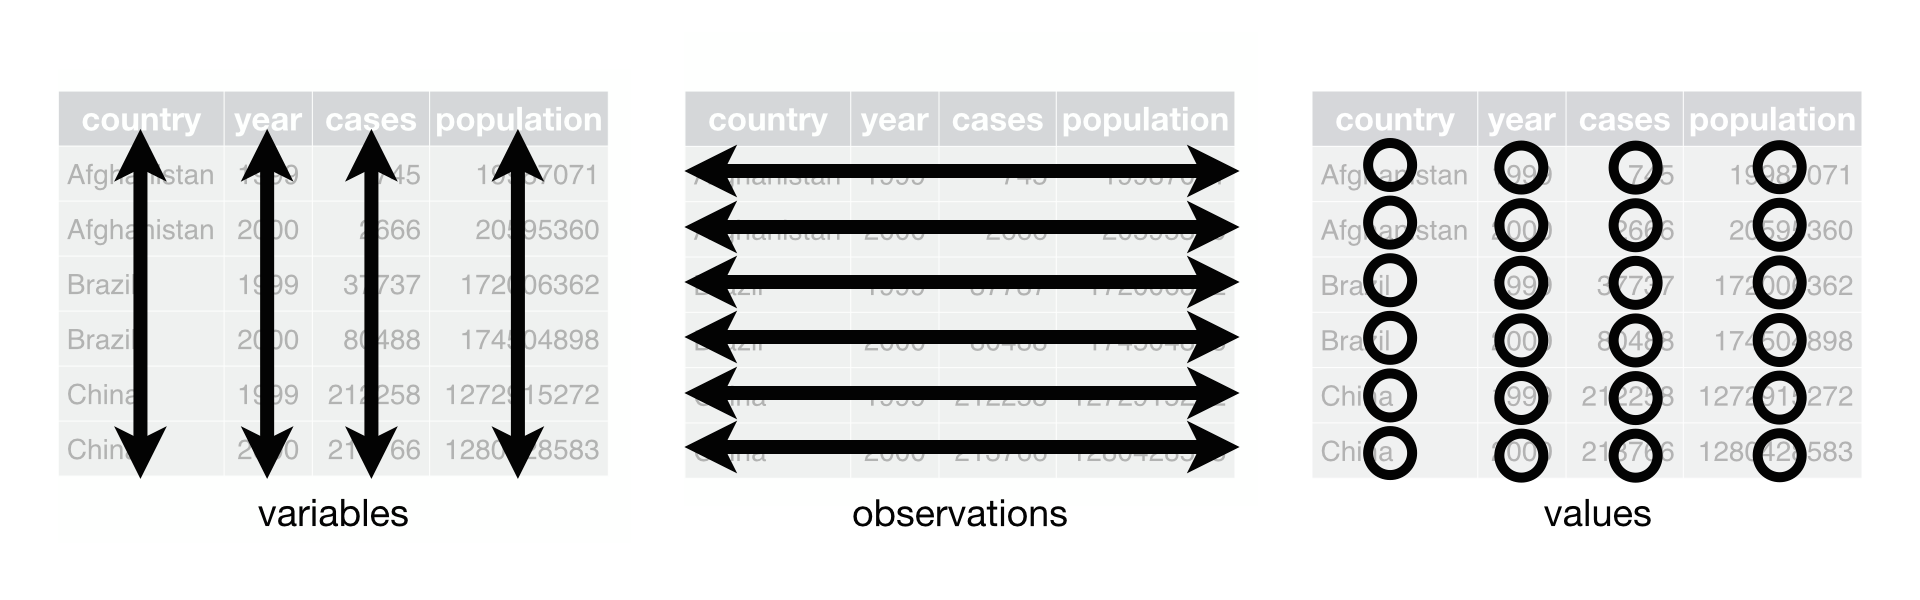
\includegraphics{index_files/mediabag/tidy-1.png}

}

\caption{tidy data}

\end{figure}%

この章では、データを整然な形に整形する方法と、もともとのデータを整然データへ変換する手順を紹介する。

ここでは tidyverse を中心に作業を進める。

\begin{Shaded}
\begin{Highlighting}[]
\FunctionTok{library}\NormalTok{(tidyverse)}
\end{Highlighting}
\end{Shaded}

特に \texttt{dplyr} と \texttt{tidyr} の機能を活用する。

\section{データ整形}\label{ux30c7ux30fcux30bfux6574ux5f62}

まずデータセット \texttt{mtcars}
を例に取り、整形の基本操作を確認する。\texttt{as\_tibble()}
を介して行名を列に移すと、後続の操作が行いやすくなる。

\begin{Shaded}
\begin{Highlighting}[]
\NormalTok{mtcars\_tbl }\OtherTok{\textless{}{-}}\NormalTok{ mtcars }\SpecialCharTok{|\textgreater{}} 
  \FunctionTok{as\_tibble}\NormalTok{(}\AttributeTok{rownames =} \StringTok{"model"}\NormalTok{)}

\NormalTok{mtcars\_tbl }\SpecialCharTok{|\textgreater{}} \FunctionTok{slice\_head}\NormalTok{(}\AttributeTok{n =} \DecValTok{6}\NormalTok{)}
\DocumentationTok{\#\# \# A tibble: 6 x 12}
\DocumentationTok{\#\#   model          mpg   cyl  disp    hp  drat    wt  qsec    vs    am  gear  carb}
\DocumentationTok{\#\#   \textless{}chr\textgreater{}        \textless{}dbl\textgreater{} \textless{}dbl\textgreater{} \textless{}dbl\textgreater{} \textless{}dbl\textgreater{} \textless{}dbl\textgreater{} \textless{}dbl\textgreater{} \textless{}dbl\textgreater{} \textless{}dbl\textgreater{} \textless{}dbl\textgreater{} \textless{}dbl\textgreater{} \textless{}dbl\textgreater{}}
\DocumentationTok{\#\# 1 Mazda RX4     21       6   160   110  3.9   2.62  16.5     0     1     4     4}
\DocumentationTok{\#\# 2 Mazda RX4 W\textasciitilde{}  21       6   160   110  3.9   2.88  17.0     0     1     4     4}
\DocumentationTok{\#\# 3 Datsun 710    22.8     4   108    93  3.85  2.32  18.6     1     1     4     1}
\DocumentationTok{\#\# 4 Hornet 4 Dr\textasciitilde{}  21.4     6   258   110  3.08  3.22  19.4     1     0     3     1}
\DocumentationTok{\#\# 5 Hornet Spor\textasciitilde{}  18.7     8   360   175  3.15  3.44  17.0     0     0     3     2}
\DocumentationTok{\#\# 6 Valiant       18.1     6   225   105  2.76  3.46  20.2     1     0     3     1}
\end{Highlighting}
\end{Shaded}

ここでは R 4.1 から導入されたパイプ演算子
\texttt{\textbar{}\textgreater{}} を利用している。従来の
\texttt{\%\textgreater{}\%}
と同様に、左辺の結果を右辺の関数に渡す構文である。

\texttt{dplyr} を使うとデータフレームの処理が大幅に簡潔になる。
変数の抽出には \texttt{select()} を使う。

\begin{Shaded}
\begin{Highlighting}[]
\NormalTok{mtcars\_tbl }\SpecialCharTok{|\textgreater{}} 
  \FunctionTok{select}\NormalTok{(model, mpg, disp) }\SpecialCharTok{|\textgreater{}} 
  \FunctionTok{slice\_head}\NormalTok{(}\AttributeTok{n =} \DecValTok{6}\NormalTok{)}
\DocumentationTok{\#\# \# A tibble: 6 x 3}
\DocumentationTok{\#\#   model               mpg  disp}
\DocumentationTok{\#\#   \textless{}chr\textgreater{}             \textless{}dbl\textgreater{} \textless{}dbl\textgreater{}}
\DocumentationTok{\#\# 1 Mazda RX4          21     160}
\DocumentationTok{\#\# 2 Mazda RX4 Wag      21     160}
\DocumentationTok{\#\# 3 Datsun 710         22.8   108}
\DocumentationTok{\#\# 4 Hornet 4 Drive     21.4   258}
\DocumentationTok{\#\# 5 Hornet Sportabout  18.7   360}
\DocumentationTok{\#\# 6 Valiant            18.1   225}
\end{Highlighting}
\end{Shaded}

条件に合致した行だけを抽出したい場合は \texttt{filter()} が便利である。

\begin{Shaded}
\begin{Highlighting}[]
\NormalTok{mtcars\_tbl }\SpecialCharTok{|\textgreater{}} 
  \FunctionTok{select}\NormalTok{(model, mpg, disp) }\SpecialCharTok{|\textgreater{}} 
  \FunctionTok{filter}\NormalTok{(disp }\SpecialCharTok{\textgreater{}} \DecValTok{300}\NormalTok{)}
\DocumentationTok{\#\# \# A tibble: 11 x 3}
\DocumentationTok{\#\#    model                 mpg  disp}
\DocumentationTok{\#\#    \textless{}chr\textgreater{}               \textless{}dbl\textgreater{} \textless{}dbl\textgreater{}}
\DocumentationTok{\#\#  1 Hornet Sportabout    18.7   360}
\DocumentationTok{\#\#  2 Duster 360           14.3   360}
\DocumentationTok{\#\#  3 Cadillac Fleetwood   10.4   472}
\DocumentationTok{\#\#  4 Lincoln Continental  10.4   460}
\DocumentationTok{\#\#  5 Chrysler Imperial    14.7   440}
\DocumentationTok{\#\#  6 Dodge Challenger     15.5   318}
\DocumentationTok{\#\#  7 AMC Javelin          15.2   304}
\DocumentationTok{\#\#  8 Camaro Z28           13.3   350}
\DocumentationTok{\#\#  9 Pontiac Firebird     19.2   400}
\DocumentationTok{\#\# 10 Ford Pantera L       15.8   351}
\DocumentationTok{\#\# 11 Maserati Bora        15     301}
\end{Highlighting}
\end{Shaded}

\texttt{rename()}
を使えば変数名を変更できる。日本語の列名にも対応している。

\begin{Shaded}
\begin{Highlighting}[]
\NormalTok{mtcars\_tbl }\SpecialCharTok{|\textgreater{}} 
  \FunctionTok{select}\NormalTok{(model, mpg, disp) }\SpecialCharTok{|\textgreater{}} 
  \FunctionTok{rename}\NormalTok{(}\StringTok{\textasciigrave{}}\AttributeTok{速度}\StringTok{\textasciigrave{}} \OtherTok{=}\NormalTok{ mpg, }\StringTok{\textasciigrave{}}\AttributeTok{距離}\StringTok{\textasciigrave{}} \OtherTok{=}\NormalTok{ disp) }\SpecialCharTok{|\textgreater{}} 
  \FunctionTok{slice\_head}\NormalTok{(}\AttributeTok{n =} \DecValTok{6}\NormalTok{)}
\DocumentationTok{\#\# \# A tibble: 6 x 3}
\DocumentationTok{\#\#   model             \textasciigrave{}\textless{}U+901F\textgreater{}\textless{}U+5EA6\textgreater{}\textasciigrave{} \textasciigrave{}\textless{}U+8DDD\textgreater{}\textless{}U+96E2\textgreater{}\textasciigrave{}}
\DocumentationTok{\#\#   \textless{}chr\textgreater{}              \textless{}dbl\textgreater{}  \textless{}dbl\textgreater{}}
\DocumentationTok{\#\# 1 Mazda RX4           21      160}
\DocumentationTok{\#\# 2 Mazda RX4 Wag       21      160}
\DocumentationTok{\#\# 3 Datsun 710          22.8    108}
\DocumentationTok{\#\# 4 Hornet 4 Drive      21.4    258}
\DocumentationTok{\#\# 5 Hornet Sportabout   18.7    360}
\DocumentationTok{\#\# 6 Valiant             18.1    225}
\end{Highlighting}
\end{Shaded}

並べ替えは \texttt{arrange()} で行う。

\begin{Shaded}
\begin{Highlighting}[]
\NormalTok{mtcars\_tbl }\SpecialCharTok{|\textgreater{}} 
  \FunctionTok{select}\NormalTok{(model, mpg, disp) }\SpecialCharTok{|\textgreater{}} 
  \FunctionTok{arrange}\NormalTok{(mpg) }\SpecialCharTok{|\textgreater{}} 
  \FunctionTok{slice\_head}\NormalTok{(}\AttributeTok{n =} \DecValTok{6}\NormalTok{)}
\DocumentationTok{\#\# \# A tibble: 6 x 3}
\DocumentationTok{\#\#   model                 mpg  disp}
\DocumentationTok{\#\#   \textless{}chr\textgreater{}               \textless{}dbl\textgreater{} \textless{}dbl\textgreater{}}
\DocumentationTok{\#\# 1 Cadillac Fleetwood   10.4   472}
\DocumentationTok{\#\# 2 Lincoln Continental  10.4   460}
\DocumentationTok{\#\# 3 Camaro Z28           13.3   350}
\DocumentationTok{\#\# 4 Duster 360           14.3   360}
\DocumentationTok{\#\# 5 Chrysler Imperial    14.7   440}
\DocumentationTok{\#\# 6 Maserati Bora        15     301}
\end{Highlighting}
\end{Shaded}

降順に並べる場合は \texttt{desc()} と組み合わせる。

\begin{Shaded}
\begin{Highlighting}[]
\NormalTok{mtcars\_tbl }\SpecialCharTok{|\textgreater{}} 
  \FunctionTok{select}\NormalTok{(model, mpg, disp) }\SpecialCharTok{|\textgreater{}} 
  \FunctionTok{arrange}\NormalTok{(}\FunctionTok{desc}\NormalTok{(mpg)) }\SpecialCharTok{|\textgreater{}} 
  \FunctionTok{slice\_head}\NormalTok{(}\AttributeTok{n =} \DecValTok{6}\NormalTok{)}
\DocumentationTok{\#\# \# A tibble: 6 x 3}
\DocumentationTok{\#\#   model            mpg  disp}
\DocumentationTok{\#\#   \textless{}chr\textgreater{}          \textless{}dbl\textgreater{} \textless{}dbl\textgreater{}}
\DocumentationTok{\#\# 1 Toyota Corolla  33.9  71.1}
\DocumentationTok{\#\# 2 Fiat 128        32.4  78.7}
\DocumentationTok{\#\# 3 Honda Civic     30.4  75.7}
\DocumentationTok{\#\# 4 Lotus Europa    30.4  95.1}
\DocumentationTok{\#\# 5 Fiat X1{-}9       27.3  79  }
\DocumentationTok{\#\# 6 Porsche 914{-}2   26   120.}
\end{Highlighting}
\end{Shaded}

\texttt{mutate()} を使うと新しい列を追加できる。

\begin{Shaded}
\begin{Highlighting}[]
\NormalTok{mtcars\_tbl }\SpecialCharTok{|\textgreater{}} 
  \FunctionTok{mutate}\NormalTok{(}\AttributeTok{gpm =} \DecValTok{1} \SpecialCharTok{/}\NormalTok{ mpg) }\SpecialCharTok{|\textgreater{}} 
  \FunctionTok{select}\NormalTok{(model, mpg, gpm) }\SpecialCharTok{|\textgreater{}} 
  \FunctionTok{slice\_head}\NormalTok{(}\AttributeTok{n =} \DecValTok{6}\NormalTok{)}
\DocumentationTok{\#\# \# A tibble: 6 x 3}
\DocumentationTok{\#\#   model               mpg    gpm}
\DocumentationTok{\#\#   \textless{}chr\textgreater{}             \textless{}dbl\textgreater{}  \textless{}dbl\textgreater{}}
\DocumentationTok{\#\# 1 Mazda RX4          21   0.0476}
\DocumentationTok{\#\# 2 Mazda RX4 Wag      21   0.0476}
\DocumentationTok{\#\# 3 Datsun 710         22.8 0.0439}
\DocumentationTok{\#\# 4 Hornet 4 Drive     21.4 0.0467}
\DocumentationTok{\#\# 5 Hornet Sportabout  18.7 0.0535}
\DocumentationTok{\#\# 6 Valiant            18.1 0.0552}
\end{Highlighting}
\end{Shaded}

\texttt{mutate()}
は既存列の上書きや複数列の同時作成も可能で、計算や条件分岐をまとめて記述できる点が強みである。

次の例では、\texttt{mpg} が 20 を超える場合に \texttt{TRUE}
を返すブール列を追加している。

\begin{Shaded}
\begin{Highlighting}[]
\NormalTok{mtcars\_tbl }\SpecialCharTok{|\textgreater{}} 
  \FunctionTok{mutate}\NormalTok{(}\AttributeTok{is\_high\_mileage =}\NormalTok{ mpg }\SpecialCharTok{\textgreater{}} \DecValTok{20}\NormalTok{) }\SpecialCharTok{|\textgreater{}} 
  \FunctionTok{select}\NormalTok{(model, mpg, is\_high\_mileage) }\SpecialCharTok{|\textgreater{}} 
  \FunctionTok{slice\_head}\NormalTok{(}\AttributeTok{n =} \DecValTok{6}\NormalTok{)}
\DocumentationTok{\#\# \# A tibble: 6 x 3}
\DocumentationTok{\#\#   model               mpg is\_high\_mileage}
\DocumentationTok{\#\#   \textless{}chr\textgreater{}             \textless{}dbl\textgreater{} \textless{}lgl\textgreater{}          }
\DocumentationTok{\#\# 1 Mazda RX4          21   TRUE           }
\DocumentationTok{\#\# 2 Mazda RX4 Wag      21   TRUE           }
\DocumentationTok{\#\# 3 Datsun 710         22.8 TRUE           }
\DocumentationTok{\#\# 4 Hornet 4 Drive     21.4 TRUE           }
\DocumentationTok{\#\# 5 Hornet Sportabout  18.7 FALSE          }
\DocumentationTok{\#\# 6 Valiant            18.1 FALSE}
\end{Highlighting}
\end{Shaded}

\texttt{summarise()} で基本統計量を算出できる。

\begin{Shaded}
\begin{Highlighting}[]
\NormalTok{mtcars\_tbl }\SpecialCharTok{|\textgreater{}} 
  \FunctionTok{summarise}\NormalTok{(}\AttributeTok{avg =} \FunctionTok{mean}\NormalTok{(mpg), }
            \AttributeTok{sd  =} \FunctionTok{sd}\NormalTok{(mpg), }
            \AttributeTok{.groups =} \StringTok{"drop"}\NormalTok{)}
\DocumentationTok{\#\# \# A tibble: 1 x 2}
\DocumentationTok{\#\#     avg    sd}
\DocumentationTok{\#\#   \textless{}dbl\textgreater{} \textless{}dbl\textgreater{}}
\DocumentationTok{\#\# 1  20.1  6.03}
\end{Highlighting}
\end{Shaded}

列名を任意に付けておけば、後続の処理で指標を参照しやすくなる。

\texttt{summarise()} に \texttt{.by}
を指定すれば、グループごとの集計も容易である。

\begin{Shaded}
\begin{Highlighting}[]
\NormalTok{mtcars\_tbl }\SpecialCharTok{|\textgreater{}} 
  \FunctionTok{summarise}\NormalTok{(}
    \AttributeTok{n   =} \FunctionTok{n}\NormalTok{(),}
    \AttributeTok{avg =} \FunctionTok{mean}\NormalTok{(mpg),}
    \AttributeTok{sd  =} \FunctionTok{sd}\NormalTok{(mpg),}
    \AttributeTok{.by =}\NormalTok{ cyl}
\NormalTok{  )}
\DocumentationTok{\#\# \# A tibble: 3 x 4}
\DocumentationTok{\#\#     cyl     n   avg    sd}
\DocumentationTok{\#\#   \textless{}dbl\textgreater{} \textless{}int\textgreater{} \textless{}dbl\textgreater{} \textless{}dbl\textgreater{}}
\DocumentationTok{\#\# 1     6     7  19.7  1.45}
\DocumentationTok{\#\# 2     4    11  26.7  4.51}
\DocumentationTok{\#\# 3     8    14  15.1  2.56}
\end{Highlighting}
\end{Shaded}

\section{データ結合}\label{ux30c7ux30fcux30bfux7d50ux5408}

\texttt{dplyr}
にはデータフレームを縦横方向に結合したり、キーを用いて結合したりするための関数が揃っている。

縦方向に結合するには \texttt{bind\_rows()} を使う。

\begin{Shaded}
\begin{Highlighting}[]
\NormalTok{df1 }\OtherTok{\textless{}{-}} \FunctionTok{tibble}\NormalTok{(}\AttributeTok{X =} \DecValTok{1}\SpecialCharTok{:}\DecValTok{2}\NormalTok{, }\AttributeTok{Y =} \DecValTok{1}\SpecialCharTok{:}\DecValTok{2}\NormalTok{)}
\NormalTok{df2 }\OtherTok{\textless{}{-}} \FunctionTok{tibble}\NormalTok{(}\AttributeTok{X =} \DecValTok{4}\NormalTok{,   }\AttributeTok{Y =} \DecValTok{4}\NormalTok{)}

\FunctionTok{bind\_rows}\NormalTok{(df1, df2)}
\DocumentationTok{\#\# \# A tibble: 3 x 2}
\DocumentationTok{\#\#       X     Y}
\DocumentationTok{\#\#   \textless{}dbl\textgreater{} \textless{}dbl\textgreater{}}
\DocumentationTok{\#\# 1     1     1}
\DocumentationTok{\#\# 2     2     2}
\DocumentationTok{\#\# 3     4     4}
\end{Highlighting}
\end{Shaded}

列名と型が一致していれば、欠けている列には自動で \texttt{NA}
が補われる。

横方向に結合する場合は \texttt{bind\_cols()} を利用する。

\begin{Shaded}
\begin{Highlighting}[]
\NormalTok{df3 }\OtherTok{\textless{}{-}} \FunctionTok{tibble}\NormalTok{(}\AttributeTok{Z =} \DecValTok{5}\SpecialCharTok{:}\DecValTok{6}\NormalTok{)}
\FunctionTok{bind\_cols}\NormalTok{(df1, df3)}
\DocumentationTok{\#\# \# A tibble: 2 x 3}
\DocumentationTok{\#\#       X     Y     Z}
\DocumentationTok{\#\#   \textless{}int\textgreater{} \textless{}int\textgreater{} \textless{}int\textgreater{}}
\DocumentationTok{\#\# 1     1     1     5}
\DocumentationTok{\#\# 2     2     2     6}
\end{Highlighting}
\end{Shaded}

行数が一致していないとリサイクルされるか警告が出るので注意する。

キーを用いた結合には四種類の join 関数が利用できる。

\begin{Shaded}
\begin{Highlighting}[]
\NormalTok{dfx }\OtherTok{\textless{}{-}} \FunctionTok{tibble}\NormalTok{(}\AttributeTok{id =} \FunctionTok{c}\NormalTok{(}\StringTok{"A"}\NormalTok{, }\StringTok{"B"}\NormalTok{, }\StringTok{"C"}\NormalTok{), }\AttributeTok{X =} \DecValTok{1}\SpecialCharTok{:}\DecValTok{3}\NormalTok{)}
\NormalTok{dfy }\OtherTok{\textless{}{-}} \FunctionTok{tibble}\NormalTok{(}\AttributeTok{id =} \FunctionTok{c}\NormalTok{(}\StringTok{"A"}\NormalTok{, }\StringTok{"B"}\NormalTok{, }\StringTok{"D"}\NormalTok{), }\AttributeTok{Y =} \FunctionTok{c}\NormalTok{(}\ConstantTok{TRUE}\NormalTok{, }\ConstantTok{FALSE}\NormalTok{, }\ConstantTok{TRUE}\NormalTok{))}
\end{Highlighting}
\end{Shaded}

左側データ(\texttt{dfx})の行をすべて保持して結合するには
\texttt{left\_join()} を用いる。

\begin{Shaded}
\begin{Highlighting}[]
\FunctionTok{left\_join}\NormalTok{(dfx, dfy, }\AttributeTok{by =} \StringTok{"id"}\NormalTok{)}
\DocumentationTok{\#\# \# A tibble: 3 x 3}
\DocumentationTok{\#\#   id        X Y    }
\DocumentationTok{\#\#   \textless{}chr\textgreater{} \textless{}int\textgreater{} \textless{}lgl\textgreater{}}
\DocumentationTok{\#\# 1 A         1 TRUE }
\DocumentationTok{\#\# 2 B         2 FALSE}
\DocumentationTok{\#\# 3 C         3 NA}
\end{Highlighting}
\end{Shaded}

右側データ(\texttt{dfy})の行をすべて保持するなら
\texttt{right\_join()}。

\begin{Shaded}
\begin{Highlighting}[]
\FunctionTok{right\_join}\NormalTok{(dfx, dfy, }\AttributeTok{by =} \StringTok{"id"}\NormalTok{)}
\DocumentationTok{\#\# \# A tibble: 3 x 3}
\DocumentationTok{\#\#   id        X Y    }
\DocumentationTok{\#\#   \textless{}chr\textgreater{} \textless{}int\textgreater{} \textless{}lgl\textgreater{}}
\DocumentationTok{\#\# 1 A         1 TRUE }
\DocumentationTok{\#\# 2 B         2 FALSE}
\DocumentationTok{\#\# 3 D        NA TRUE}
\end{Highlighting}
\end{Shaded}

両方の行をすべて保持するなら \texttt{full\_join()}。

\begin{Shaded}
\begin{Highlighting}[]
\FunctionTok{full\_join}\NormalTok{(dfx, dfy, }\AttributeTok{by =} \StringTok{"id"}\NormalTok{)}
\DocumentationTok{\#\# \# A tibble: 4 x 3}
\DocumentationTok{\#\#   id        X Y    }
\DocumentationTok{\#\#   \textless{}chr\textgreater{} \textless{}int\textgreater{} \textless{}lgl\textgreater{}}
\DocumentationTok{\#\# 1 A         1 TRUE }
\DocumentationTok{\#\# 2 B         2 FALSE}
\DocumentationTok{\#\# 3 C         3 NA   }
\DocumentationTok{\#\# 4 D        NA TRUE}
\end{Highlighting}
\end{Shaded}

\texttt{inner\_join()} は共通部分のみを抽出する。

\begin{Shaded}
\begin{Highlighting}[]
\FunctionTok{inner\_join}\NormalTok{(dfx, dfy, }\AttributeTok{by =} \StringTok{"id"}\NormalTok{)}
\DocumentationTok{\#\# \# A tibble: 2 x 3}
\DocumentationTok{\#\#   id        X Y    }
\DocumentationTok{\#\#   \textless{}chr\textgreater{} \textless{}int\textgreater{} \textless{}lgl\textgreater{}}
\DocumentationTok{\#\# 1 A         1 TRUE }
\DocumentationTok{\#\# 2 B         2 FALSE}
\end{Highlighting}
\end{Shaded}

より複雑な条件で結合したい場合は \texttt{join\_by()}
を使うと柔軟に定義できる。 複雑な条件で結合したい場合は
\texttt{join\_by()} を使うと柔軟に定義できる。

\section{tidyr}\label{tidyr}

ここからは \texttt{tidyr}
による整形の例を紹介する。まず次のデータセットを用意する。

\begin{Shaded}
\begin{Highlighting}[]
\NormalTok{df }\OtherTok{\textless{}{-}} \FunctionTok{tibble}\NormalTok{(}
  \AttributeTok{time =} \DecValTok{2010}\SpecialCharTok{:}\DecValTok{2014}\NormalTok{,}
  \AttributeTok{X =} \FunctionTok{rnorm}\NormalTok{(}\DecValTok{5}\NormalTok{, }\DecValTok{0}\NormalTok{, }\DecValTok{1}\NormalTok{),}
  \AttributeTok{Y =} \FunctionTok{rnorm}\NormalTok{(}\DecValTok{5}\NormalTok{, }\DecValTok{0}\NormalTok{, }\DecValTok{2}\NormalTok{),}
  \AttributeTok{Z =} \FunctionTok{rnorm}\NormalTok{(}\DecValTok{5}\NormalTok{, }\DecValTok{0}\NormalTok{, }\DecValTok{4}\NormalTok{)}
\NormalTok{)}
\CommentTok{\# \textasciigrave{}tibble()\textasciigrave{} なら列の型を意識しつつ手早くサンプル値を用意できる}
\NormalTok{df }\SpecialCharTok{|\textgreater{}} \FunctionTok{slice\_head}\NormalTok{(}\AttributeTok{n =} \DecValTok{6}\NormalTok{)}
\DocumentationTok{\#\# \# A tibble: 5 x 4}
\DocumentationTok{\#\#    time       X      Y      Z}
\DocumentationTok{\#\#   \textless{}int\textgreater{}   \textless{}dbl\textgreater{}  \textless{}dbl\textgreater{}  \textless{}dbl\textgreater{}}
\DocumentationTok{\#\# 1  2010  0.889   0.610  8.04 }
\DocumentationTok{\#\# 2  2011 {-}0.863  {-}3.42  {-}0.189}
\DocumentationTok{\#\# 3  2012  0.675   0.823  5.15 }
\DocumentationTok{\#\# 4  2013  0.0851 {-}4.55   2.10 }
\DocumentationTok{\#\# 5  2014  0.489   1.49  {-}7.48}
\end{Highlighting}
\end{Shaded}

列名をキーにして縦長へ変換するときは \texttt{pivot\_longer()} を用いる。

\begin{Shaded}
\begin{Highlighting}[]
\NormalTok{df\_long }\OtherTok{\textless{}{-}}\NormalTok{ df }\SpecialCharTok{|\textgreater{}} 
  \FunctionTok{pivot\_longer}\NormalTok{(}\SpecialCharTok{{-}}\NormalTok{time, }\AttributeTok{names\_to =} \StringTok{"key"}\NormalTok{, }\AttributeTok{values\_to =} \StringTok{"value"}\NormalTok{)}
\CommentTok{\# names\_to / values\_to を指定しておくと後続処理が読みやすい}
\NormalTok{df\_long}
\DocumentationTok{\#\# \# A tibble: 15 x 3}
\DocumentationTok{\#\#     time key     value}
\DocumentationTok{\#\#    \textless{}int\textgreater{} \textless{}chr\textgreater{}   \textless{}dbl\textgreater{}}
\DocumentationTok{\#\#  1  2010 X      0.889 }
\DocumentationTok{\#\#  2  2010 Y      0.610 }
\DocumentationTok{\#\#  3  2010 Z      8.04  }
\DocumentationTok{\#\#  4  2011 X     {-}0.863 }
\DocumentationTok{\#\#  5  2011 Y     {-}3.42  }
\DocumentationTok{\#\#  6  2011 Z     {-}0.189 }
\DocumentationTok{\#\#  7  2012 X      0.675 }
\DocumentationTok{\#\#  8  2012 Y      0.823 }
\DocumentationTok{\#\#  9  2012 Z      5.15  }
\DocumentationTok{\#\# 10  2013 X      0.0851}
\DocumentationTok{\#\# 11  2013 Y     {-}4.55  }
\DocumentationTok{\#\# 12  2013 Z      2.10  }
\DocumentationTok{\#\# 13  2014 X      0.489 }
\DocumentationTok{\#\# 14  2014 Y      1.49  }
\DocumentationTok{\#\# 15  2014 Z     {-}7.48}
\end{Highlighting}
\end{Shaded}

\texttt{pivot\_wider()} を使えば再び元の構造に戻すことができる。

\begin{Shaded}
\begin{Highlighting}[]
\NormalTok{df\_long }\SpecialCharTok{|\textgreater{}} 
  \FunctionTok{pivot\_wider}\NormalTok{(}\AttributeTok{names\_from =} \StringTok{"key"}\NormalTok{, }\AttributeTok{values\_from =} \StringTok{"value"}\NormalTok{)}
\DocumentationTok{\#\# \# A tibble: 5 x 4}
\DocumentationTok{\#\#    time       X      Y      Z}
\DocumentationTok{\#\#   \textless{}int\textgreater{}   \textless{}dbl\textgreater{}  \textless{}dbl\textgreater{}  \textless{}dbl\textgreater{}}
\DocumentationTok{\#\# 1  2010  0.889   0.610  8.04 }
\DocumentationTok{\#\# 2  2011 {-}0.863  {-}3.42  {-}0.189}
\DocumentationTok{\#\# 3  2012  0.675   0.823  5.15 }
\DocumentationTok{\#\# 4  2013  0.0851 {-}4.55   2.10 }
\DocumentationTok{\#\# 5  2014  0.489   1.49  {-}7.48}
\end{Highlighting}
\end{Shaded}

列数を増やして見せたいときや、プレゼン資料で横持ちの表が必要なときに役立つ。

\texttt{time} を列方向に展開すれば、年次を横持ちした表へ変換できる。

\begin{Shaded}
\begin{Highlighting}[]
\NormalTok{df\_wide }\OtherTok{\textless{}{-}}\NormalTok{ df\_long }\SpecialCharTok{|\textgreater{}} 
  \FunctionTok{pivot\_wider}\NormalTok{(}\AttributeTok{names\_from =} \StringTok{"time"}\NormalTok{, }\AttributeTok{values\_from =} \StringTok{"value"}\NormalTok{)}
\NormalTok{df\_wide}
\DocumentationTok{\#\# \# A tibble: 3 x 6}
\DocumentationTok{\#\#   key   \textasciigrave{}2010\textasciigrave{} \textasciigrave{}2011\textasciigrave{} \textasciigrave{}2012\textasciigrave{}  \textasciigrave{}2013\textasciigrave{} \textasciigrave{}2014\textasciigrave{}}
\DocumentationTok{\#\#   \textless{}chr\textgreater{}  \textless{}dbl\textgreater{}  \textless{}dbl\textgreater{}  \textless{}dbl\textgreater{}   \textless{}dbl\textgreater{}  \textless{}dbl\textgreater{}}
\DocumentationTok{\#\# 1 X      0.889 {-}0.863  0.675  0.0851  0.489}
\DocumentationTok{\#\# 2 Y      0.610 {-}3.42   0.823 {-}4.55    1.49 }
\DocumentationTok{\#\# 3 Z      8.04  {-}0.189  5.15   2.10   {-}7.48}
\end{Highlighting}
\end{Shaded}

再び縦長に戻す場合は次のとおりである。

\begin{Shaded}
\begin{Highlighting}[]
\NormalTok{df\_wide }\SpecialCharTok{|\textgreater{}} 
  \FunctionTok{pivot\_longer}\NormalTok{(}\SpecialCharTok{{-}}\NormalTok{key, }\AttributeTok{names\_to =} \StringTok{"time"}\NormalTok{, }\AttributeTok{values\_to =} \StringTok{"value"}\NormalTok{)}
\DocumentationTok{\#\# \# A tibble: 15 x 3}
\DocumentationTok{\#\#    key   time    value}
\DocumentationTok{\#\#    \textless{}chr\textgreater{} \textless{}chr\textgreater{}   \textless{}dbl\textgreater{}}
\DocumentationTok{\#\#  1 X     2010   0.889 }
\DocumentationTok{\#\#  2 X     2011  {-}0.863 }
\DocumentationTok{\#\#  3 X     2012   0.675 }
\DocumentationTok{\#\#  4 X     2013   0.0851}
\DocumentationTok{\#\#  5 X     2014   0.489 }
\DocumentationTok{\#\#  6 Y     2010   0.610 }
\DocumentationTok{\#\#  7 Y     2011  {-}3.42  }
\DocumentationTok{\#\#  8 Y     2012   0.823 }
\DocumentationTok{\#\#  9 Y     2013  {-}4.55  }
\DocumentationTok{\#\# 10 Y     2014   1.49  }
\DocumentationTok{\#\# 11 Z     2010   8.04  }
\DocumentationTok{\#\# 12 Z     2011  {-}0.189 }
\DocumentationTok{\#\# 13 Z     2012   5.15  }
\DocumentationTok{\#\# 14 Z     2013   2.10  }
\DocumentationTok{\#\# 15 Z     2014  {-}7.48}
\end{Highlighting}
\end{Shaded}

\texttt{pivot\_longer()} と \texttt{summarise()}
を組み合わせると、変数別の記述統計を簡潔にまとめられる。

\begin{Shaded}
\begin{Highlighting}[]
\NormalTok{cars }\SpecialCharTok{|\textgreater{}} 
  \FunctionTok{as\_tibble}\NormalTok{() }\SpecialCharTok{|\textgreater{}} 
  \FunctionTok{pivot\_longer}\NormalTok{(}\FunctionTok{everything}\NormalTok{(), }\AttributeTok{names\_to =} \StringTok{"variable"}\NormalTok{, }\AttributeTok{values\_to =} \StringTok{"value"}\NormalTok{) }\SpecialCharTok{|\textgreater{}} 
  \FunctionTok{group\_by}\NormalTok{(variable) }\SpecialCharTok{|\textgreater{}}
  \FunctionTok{summarise}\NormalTok{(}
    \AttributeTok{nobs =} \FunctionTok{n}\NormalTok{(),}
    \AttributeTok{avg  =} \FunctionTok{mean}\NormalTok{(value),}
    \AttributeTok{sd   =} \FunctionTok{sd}\NormalTok{(value)}
\NormalTok{  ) }\SpecialCharTok{|\textgreater{}}
  \FunctionTok{ungroup}\NormalTok{()}
\DocumentationTok{\#\# \# A tibble: 2 x 4}
\DocumentationTok{\#\#   variable  nobs   avg    sd}
\DocumentationTok{\#\#   \textless{}chr\textgreater{}    \textless{}int\textgreater{} \textless{}dbl\textgreater{} \textless{}dbl\textgreater{}}
\DocumentationTok{\#\# 1 dist        50  43.0 25.8 }
\DocumentationTok{\#\# 2 speed       50  15.4  5.29}
\CommentTok{\# 欠損を除外したいときは mean(value, na.rm = TRUE) のように na.rm を付ける}
\end{Highlighting}
\end{Shaded}

日本語の列名でも同じ操作が可能である。

\begin{Shaded}
\begin{Highlighting}[]
\NormalTok{tab }\OtherTok{\textless{}{-}}\NormalTok{ cars }\SpecialCharTok{|\textgreater{}} 
  \FunctionTok{as\_tibble}\NormalTok{() }\SpecialCharTok{|\textgreater{}} 
  \FunctionTok{pivot\_longer}\NormalTok{(}\FunctionTok{c}\NormalTok{(dist, speed), }\AttributeTok{names\_to =} \StringTok{"variable"}\NormalTok{, }\AttributeTok{values\_to =} \StringTok{"value"}\NormalTok{) }\SpecialCharTok{|\textgreater{}} 
  \FunctionTok{group\_by}\NormalTok{(variable) }\SpecialCharTok{|\textgreater{}}
  \FunctionTok{summarise}\NormalTok{(}
    \AttributeTok{nobs =} \FunctionTok{n}\NormalTok{(),}
    \AttributeTok{avg  =} \FunctionTok{mean}\NormalTok{(value),}
    \AttributeTok{sd   =} \FunctionTok{sd}\NormalTok{(value)}
\NormalTok{  ) }\SpecialCharTok{|\textgreater{}}
  \FunctionTok{ungroup}\NormalTok{() }\SpecialCharTok{|\textgreater{}}
  \FunctionTok{mutate}\NormalTok{(}
    \StringTok{\textasciigrave{}}\AttributeTok{変数}\StringTok{\textasciigrave{}} \OtherTok{=}\NormalTok{ dplyr}\SpecialCharTok{::}\FunctionTok{recode}\NormalTok{(variable, }\AttributeTok{dist =} \StringTok{"距離"}\NormalTok{, }\AttributeTok{speed =} \StringTok{"速度"}\NormalTok{)}
\NormalTok{  ) }\SpecialCharTok{|\textgreater{}}
  \FunctionTok{select}\NormalTok{(}
    \StringTok{\textasciigrave{}}\AttributeTok{変数}\StringTok{\textasciigrave{}}\NormalTok{,}
    \StringTok{\textasciigrave{}}\AttributeTok{観測数}\StringTok{\textasciigrave{}}   \OtherTok{=}\NormalTok{ nobs,}
    \StringTok{\textasciigrave{}}\AttributeTok{平均}\StringTok{\textasciigrave{}}     \OtherTok{=}\NormalTok{ avg,}
    \StringTok{\textasciigrave{}}\AttributeTok{標準偏差}\StringTok{\textasciigrave{}} \OtherTok{=}\NormalTok{ sd}
\NormalTok{  )}
\NormalTok{tab }\SpecialCharTok{|\textgreater{}} \FunctionTok{slice\_head}\NormalTok{(}\AttributeTok{n =} \DecValTok{6}\NormalTok{)}
\DocumentationTok{\#\# \# A tibble: 2 x 4}
\DocumentationTok{\#\#   \textasciigrave{}\textless{}U+5909\textgreater{}\textless{}U+6570\textgreater{}\textasciigrave{}           \textasciigrave{}\textless{}U+89B3\textgreater{}\textless{}U+6E2C\textgreater{}\textless{}U+6570\textgreater{}\textasciigrave{} \textasciigrave{}\textless{}U+5E73\textgreater{}\textless{}U+5747\textgreater{}\textasciigrave{} \textasciigrave{}\textless{}U+6A19\textgreater{}\textless{}U+6E96\textgreater{}\textless{}U+504F\textgreater{}\textless{}U+5DEE\textgreater{}\textasciigrave{}}
\DocumentationTok{\#\#   \textless{}chr\textgreater{}               \textless{}int\textgreater{}  \textless{}dbl\textgreater{}      \textless{}dbl\textgreater{}}
\DocumentationTok{\#\# 1 \textless{}U+8DDD\textgreater{}\textless{}U+96E2\textgreater{}       50   43.0      25.8 }
\DocumentationTok{\#\# 2 \textless{}U+901F\textgreater{}\textless{}U+5EA6\textgreater{}       50   15.4       5.29}
\end{Highlighting}
\end{Shaded}

\section{実践例}\label{ux5b9fux8df5ux4f8b}

tidyr を用いた別の例を見てみよう。横軸を年としたデータセット \texttt{df}
がある。

\begin{Shaded}
\begin{Highlighting}[]
\NormalTok{df }\OtherTok{\textless{}{-}} \FunctionTok{tibble}\NormalTok{(}
  \AttributeTok{name  =}\NormalTok{ letters,}
  \StringTok{\textasciigrave{}}\AttributeTok{2010}\StringTok{\textasciigrave{}} \OtherTok{=} \FunctionTok{rnorm}\NormalTok{(}\DecValTok{26}\NormalTok{),}
  \StringTok{\textasciigrave{}}\AttributeTok{2011}\StringTok{\textasciigrave{}} \OtherTok{=} \FunctionTok{rnorm}\NormalTok{(}\DecValTok{26}\NormalTok{),}
  \StringTok{\textasciigrave{}}\AttributeTok{2012}\StringTok{\textasciigrave{}} \OtherTok{=} \FunctionTok{rnorm}\NormalTok{(}\DecValTok{26}\NormalTok{)}
\NormalTok{) }
\NormalTok{df }\SpecialCharTok{|\textgreater{}} \FunctionTok{slice\_head}\NormalTok{(}\AttributeTok{n =} \DecValTok{6}\NormalTok{)}
\DocumentationTok{\#\# \# A tibble: 6 x 4}
\DocumentationTok{\#\#   name  \textasciigrave{}2010\textasciigrave{} \textasciigrave{}2011\textasciigrave{}  \textasciigrave{}2012\textasciigrave{}}
\DocumentationTok{\#\#   \textless{}chr\textgreater{}  \textless{}dbl\textgreater{}  \textless{}dbl\textgreater{}   \textless{}dbl\textgreater{}}
\DocumentationTok{\#\# 1 a     {-}1.46  {-}0.791 {-}1.11  }
\DocumentationTok{\#\# 2 b      0.726 {-}1.47  {-}1.43  }
\DocumentationTok{\#\# 3 c      1.22  {-}0.744 {-}0.0532}
\DocumentationTok{\#\# 4 d     {-}1.62   1.21  {-}0.477 }
\DocumentationTok{\#\# 5 e      0.446 {-}1.06   0.343 }
\DocumentationTok{\#\# 6 f      0.382 {-}0.580 {-}0.690}
\end{Highlighting}
\end{Shaded}

さらに、年ごとのデータセット
\texttt{df\_2010}、\texttt{df\_2011}、\texttt{df\_2012} の 3
つも用意する。

\begin{Shaded}
\begin{Highlighting}[]
\NormalTok{df\_2010 }\OtherTok{\textless{}{-}} \FunctionTok{tibble}\NormalTok{(}\AttributeTok{name =}\NormalTok{ letters, }\AttributeTok{runif =} \FunctionTok{runif}\NormalTok{(}\DecValTok{26}\NormalTok{))}
\NormalTok{df\_2011 }\OtherTok{\textless{}{-}} \FunctionTok{tibble}\NormalTok{(}\AttributeTok{name =}\NormalTok{ letters, }\AttributeTok{runif =} \FunctionTok{runif}\NormalTok{(}\DecValTok{26}\NormalTok{))}
\NormalTok{df\_2012 }\OtherTok{\textless{}{-}} \FunctionTok{tibble}\NormalTok{(}\AttributeTok{name =}\NormalTok{ letters, }\AttributeTok{runif =} \FunctionTok{runif}\NormalTok{(}\DecValTok{26}\NormalTok{))}
\end{Highlighting}
\end{Shaded}

これら 4 つのデータセットを統合して整然データにする。

まず \texttt{df} を \texttt{pivot\_longer()} で縦長に変換する。

\begin{Shaded}
\begin{Highlighting}[]
\NormalTok{df\_rnorm }\OtherTok{\textless{}{-}}\NormalTok{ df }\SpecialCharTok{|\textgreater{}} 
  \FunctionTok{pivot\_longer}\NormalTok{(}\SpecialCharTok{{-}}\NormalTok{name, }\AttributeTok{names\_to =} \StringTok{"time"}\NormalTok{, }\AttributeTok{values\_to =} \StringTok{"rnorm"}\NormalTok{) }\SpecialCharTok{|\textgreater{}} 
  \FunctionTok{mutate}\NormalTok{(}\AttributeTok{time =} \FunctionTok{as.numeric}\NormalTok{(time))}
\NormalTok{df\_rnorm }\SpecialCharTok{|\textgreater{}} \FunctionTok{slice\_head}\NormalTok{(}\AttributeTok{n =} \DecValTok{6}\NormalTok{)}
\DocumentationTok{\#\# \# A tibble: 6 x 3}
\DocumentationTok{\#\#   name   time  rnorm}
\DocumentationTok{\#\#   \textless{}chr\textgreater{} \textless{}dbl\textgreater{}  \textless{}dbl\textgreater{}}
\DocumentationTok{\#\# 1 a      2010 {-}1.46 }
\DocumentationTok{\#\# 2 a      2011 {-}0.791}
\DocumentationTok{\#\# 3 a      2012 {-}1.11 }
\DocumentationTok{\#\# 4 b      2010  0.726}
\DocumentationTok{\#\# 5 b      2011 {-}1.47 }
\DocumentationTok{\#\# 6 b      2012 {-}1.43}
\end{Highlighting}
\end{Shaded}

ここでは \texttt{time} 列を数値に変換している。

次に、3 つの年別データセットを \texttt{bind\_rows()} で縦に結合する。

\begin{Shaded}
\begin{Highlighting}[]
\NormalTok{df\_runif }\OtherTok{\textless{}{-}} \FunctionTok{bind\_rows}\NormalTok{(}
  \StringTok{"2010"} \OtherTok{=}\NormalTok{ df\_2010,}
  \StringTok{"2011"} \OtherTok{=}\NormalTok{ df\_2011,}
  \StringTok{"2012"} \OtherTok{=}\NormalTok{ df\_2012,}
  \AttributeTok{.id    =} \StringTok{"time"}
\NormalTok{) }\SpecialCharTok{|\textgreater{}} 
  \FunctionTok{mutate}\NormalTok{(}\AttributeTok{time =} \FunctionTok{as.numeric}\NormalTok{(time))}
\NormalTok{df\_runif }\SpecialCharTok{|\textgreater{}} \FunctionTok{slice\_head}\NormalTok{(}\AttributeTok{n =} \DecValTok{6}\NormalTok{)}
\DocumentationTok{\#\# \# A tibble: 6 x 3}
\DocumentationTok{\#\#    time name  runif}
\DocumentationTok{\#\#   \textless{}dbl\textgreater{} \textless{}chr\textgreater{} \textless{}dbl\textgreater{}}
\DocumentationTok{\#\# 1  2010 a     0.191}
\DocumentationTok{\#\# 2  2010 b     0.475}
\DocumentationTok{\#\# 3  2010 c     0.208}
\DocumentationTok{\#\# 4  2010 d     0.467}
\DocumentationTok{\#\# 5  2010 e     0.738}
\DocumentationTok{\#\# 6  2010 f     0.986}
\end{Highlighting}
\end{Shaded}

\texttt{.id} で追加された列を数値に変換して年情報として利用している。

最後に \texttt{full\_join()} を使って 2 つのデータを結合する。

\begin{Shaded}
\begin{Highlighting}[]
\NormalTok{df\_full }\OtherTok{\textless{}{-}} \FunctionTok{full\_join}\NormalTok{(df\_rnorm, df\_runif, }\AttributeTok{by =} \FunctionTok{c}\NormalTok{(}\StringTok{"name"}\NormalTok{, }\StringTok{"time"}\NormalTok{))}
\NormalTok{df\_full }\SpecialCharTok{|\textgreater{}} \FunctionTok{slice\_head}\NormalTok{(}\AttributeTok{n =} \DecValTok{6}\NormalTok{)}
\DocumentationTok{\#\# \# A tibble: 6 x 4}
\DocumentationTok{\#\#   name   time  rnorm  runif}
\DocumentationTok{\#\#   \textless{}chr\textgreater{} \textless{}dbl\textgreater{}  \textless{}dbl\textgreater{}  \textless{}dbl\textgreater{}}
\DocumentationTok{\#\# 1 a      2010 {-}1.46  0.191 }
\DocumentationTok{\#\# 2 a      2011 {-}0.791 0.0829}
\DocumentationTok{\#\# 3 a      2012 {-}1.11  0.0706}
\DocumentationTok{\#\# 4 b      2010  0.726 0.475 }
\DocumentationTok{\#\# 5 b      2011 {-}1.47  0.431 }
\DocumentationTok{\#\# 6 b      2012 {-}1.43  0.269}
\end{Highlighting}
\end{Shaded}

整然データにまとめておけば、\texttt{ggplot2}
やモデリング関数へそのまま渡せるため、後続処理がスムーズになり再現性も高まる。

\bookmarksetup{startatroot}

\chapter{古典的仮定のもとでの最小二乗法}\label{ux53e4ux5178ux7684ux4eeeux5b9aux306eux3082ux3068ux3067ux306eux6700ux5c0fux4e8cux4e57ux6cd5}

\begin{Shaded}
\begin{Highlighting}[]
\FunctionTok{library}\NormalTok{(AER)}
\end{Highlighting}
\end{Shaded}

\section{単回帰モデル}\label{ux5358ux56deux5e30ux30e2ux30c7ux30eb}

まず次の単回帰モデルを考える。

\[
y = \alpha + \beta x + u
\] ここで \(x\) は説明変数、\(y\) は被説明変数、\(u\) は誤差項である。
パラメータとして \(\alpha\) は切片パラメータ, \(\beta\)
は傾きパラメータである.

以下の仮定を置く。

\begin{itemize}
\tightlist
\item
  \((x_i, y_i)\) は独立同一分布に従う。
\item
  \(E[u_i] = 0\) である。
\item
  \(u_i\) と \(x_i\) は独立である。
\item
  \(u_i\) は正規分布に従う。
\end{itemize}

これらの仮定の下では、最小二乗推定量は一致性と不偏性を持ち、さらに正規分布に従う。
一致(consistency)とは、観測数が多くなるにつれて推定量が真のパラメータに確率収束する性質である。
不偏性とは、推定量の期待値が真のパラメータに等しくなることである。
さらに、他の線形不偏推定量の中で最小の分散を持つ(BLUE: best linear
unbiased estimator)。

以降ではシミュレーションデータを用いて具体的に確認する。
ここでは標本サイズを100とし, 説明変数 \(x\)
は0から1の一様分布から生成する. 被説明変数 \(y\)
は真の切片パラメータを10, 真の傾きパラメータを2として,
正規分布の誤差項を加えて生成する. 最後にこれらのデータを
\texttt{data.frame} 関数でデータフレームにまとめる.

\begin{Shaded}
\begin{Highlighting}[]
\NormalTok{N }\OtherTok{\textless{}{-}} \DecValTok{100}
\NormalTok{x }\OtherTok{\textless{}{-}} \FunctionTok{runif}\NormalTok{(N)}
\NormalTok{y }\OtherTok{\textless{}{-}} \DecValTok{10} \SpecialCharTok{+} \DecValTok{2}\SpecialCharTok{*}\NormalTok{x }\SpecialCharTok{+} \FunctionTok{rnorm}\NormalTok{(N)}
\NormalTok{df }\OtherTok{\textless{}{-}} \FunctionTok{data.frame}\NormalTok{(x,y)}
\end{Highlighting}
\end{Shaded}

散布図を描くと次のようになる。 \texttt{plot} に
\texttt{y\ \textasciitilde{}\ x}
と指定すると、横軸に説明変数、縦軸に被説明変数を取った散布図が描かれる。

\begin{Shaded}
\begin{Highlighting}[]
\FunctionTok{plot}\NormalTok{(y}\SpecialCharTok{\textasciitilde{}}\NormalTok{x)}
\end{Highlighting}
\end{Shaded}

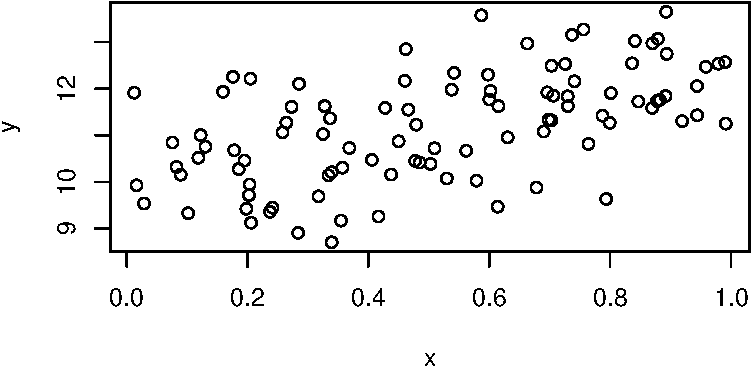
\includegraphics{07-regression1_files/figure-pdf/unnamed-chunk-3-1.pdf}

R で回帰分析を実施するには \texttt{lm} 関数を使用する.
第一引数には回帰式を \texttt{y\ \textasciitilde{}\ x}
という形式で指定し, \texttt{data} 引数にはデータフレームを指定する.
推定結果は \texttt{fm} というオブジェクトに保存する.

\begin{Shaded}
\begin{Highlighting}[]
\NormalTok{fm }\OtherTok{\textless{}{-}} \FunctionTok{lm}\NormalTok{(y }\SpecialCharTok{\textasciitilde{}}\NormalTok{ x, }\AttributeTok{data=}\NormalTok{df)}
\end{Highlighting}
\end{Shaded}

\texttt{fm} はリストとして保存されており、以下のような要素を持つ。
\texttt{typeof()} でオブジェクトの型を、\texttt{names()}
で各要素名を確認できる。

\begin{Shaded}
\begin{Highlighting}[]
\FunctionTok{typeof}\NormalTok{(fm)}
\DocumentationTok{\#\# [1] "list"}
\FunctionTok{names}\NormalTok{(fm)}
\DocumentationTok{\#\#  [1] "coefficients"  "residuals"     "effects"       "rank"         }
\DocumentationTok{\#\#  [5] "fitted.values" "assign"        "qr"            "df.residual"  }
\DocumentationTok{\#\#  [9] "xlevels"       "call"          "terms"         "model"}
\end{Highlighting}
\end{Shaded}

推定された係数 (切片と傾き) を取り出すには \texttt{coef} 関数を使用する.
\texttt{coefficients} 関数でも同じ結果が得られる
(コメントアウトしている).

\begin{Shaded}
\begin{Highlighting}[]
\FunctionTok{coef}\NormalTok{(fm)}
\DocumentationTok{\#\# (Intercept)           x }
\DocumentationTok{\#\#   10.022212    2.294907}
\CommentTok{\# coefficients(fm)}
\end{Highlighting}
\end{Shaded}

傾きの推定値は、説明変数と被説明変数の共分散を説明変数の分散で割ることで求められる。
\texttt{with} 関数を使ってデータフレーム内の変数を直接参照し,
\texttt{cov} 関数で共分散, \texttt{var} 関数で分散を計算する.

\begin{Shaded}
\begin{Highlighting}[]
\FunctionTok{with}\NormalTok{(df, }\FunctionTok{cov}\NormalTok{(x,y)}\SpecialCharTok{/}\FunctionTok{var}\NormalTok{(x))}
\DocumentationTok{\#\# [1] 2.294907}
\end{Highlighting}
\end{Shaded}

散布図に推定直線を重ねるには、まず \texttt{plot()}
で散布図を描き、続いて \texttt{abline()} に \texttt{lm}
オブジェクトを渡す。 \texttt{abline} 関数に \texttt{lm}
オブジェクトを渡すと自動的に回帰直線が描画される.

\begin{Shaded}
\begin{Highlighting}[]
\FunctionTok{plot}\NormalTok{(y}\SpecialCharTok{\textasciitilde{}}\NormalTok{x,}\AttributeTok{data=}\NormalTok{df)}
\FunctionTok{abline}\NormalTok{(fm)}
\end{Highlighting}
\end{Shaded}

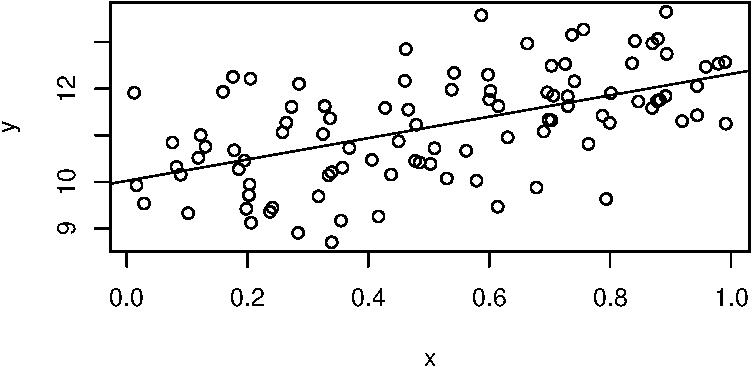
\includegraphics{07-regression1_files/figure-pdf/unnamed-chunk-8-1.pdf}

残差(実際の値と予測値の差)は \texttt{resid()} で取得できる。 ここでは
\texttt{head} 関数で最初の6つの値のみを表示している. \texttt{residuals}
関数でも同じ結果が得られる (コメントアウトしている).

\begin{Shaded}
\begin{Highlighting}[]
\FunctionTok{head}\NormalTok{(}\FunctionTok{resid}\NormalTok{(fm))}
\DocumentationTok{\#\#          1          2          3          4          5          6 }
\DocumentationTok{\#\# {-}1.0610630 {-}2.0964399 {-}1.7680508  0.8437608  1.5456126  0.1926375}
\CommentTok{\# residuals(fm)}
\CommentTok{\# with(fm, residuals)}
\end{Highlighting}
\end{Shaded}

予測値(\(38\)hat\{y\}\$)は \texttt{fitted()} によって得られる。
ここでは \texttt{head} 関数で最初の6つの値のみを表示している.
\texttt{fitted.values} でも同じ結果が得られる (コメントアウトしている).

\begin{Shaded}
\begin{Highlighting}[]
\FunctionTok{head}\NormalTok{(}\FunctionTok{fitted}\NormalTok{(fm))}
\DocumentationTok{\#\#        1        2        3        4        5        6 }
\DocumentationTok{\#\# 10.75077 10.80082 10.67351 10.77470 10.38816 11.43376}
\CommentTok{\# fitted.values(fm)}
\CommentTok{\# with(fm, fitted.values)}
\end{Highlighting}
\end{Shaded}

最小二乗法の性質として,
予測値の平均は被説明変数の平均と等しいことが知られている.
以下のコマンドで両者が一致することを確認できる.

\begin{Shaded}
\begin{Highlighting}[]
\FunctionTok{mean}\NormalTok{(}\FunctionTok{fitted}\NormalTok{(fm))}
\DocumentationTok{\#\# [1] 11.20267}
\FunctionTok{mean}\NormalTok{(df}\SpecialCharTok{$}\NormalTok{y)}
\DocumentationTok{\#\# [1] 11.20267}
\end{Highlighting}
\end{Shaded}

残差自乗和 (residual sum of squares) を計算するには \texttt{deviance}
関数を使用する. これは残差を二乗して合計した値であり,
\texttt{sum(resid(fm)\^{}2)} で直接計算することもできる.

\begin{Shaded}
\begin{Highlighting}[]
\FunctionTok{deviance}\NormalTok{(fm)}
\DocumentationTok{\#\# [1] 92.67048}
\FunctionTok{sum}\NormalTok{(}\FunctionTok{resid}\NormalTok{(fm)}\SpecialCharTok{\^{}}\DecValTok{2}\NormalTok{)}
\DocumentationTok{\#\# [1] 92.67048}
\end{Highlighting}
\end{Shaded}

残差自乗和は残差変動とも呼ばれる。
予測値の偏差の自乗和を回帰変動、被説明変数の偏差の自乗和を全変動という。
全変動は回帰変動と残差変動に分解できる(変動の分解)。 以下のコマンドで,
左辺の全変動が右辺の回帰変動と残差変動の和に等しいことを確認できる.

\begin{Shaded}
\begin{Highlighting}[]
\FunctionTok{sum}\NormalTok{((df}\SpecialCharTok{$}\NormalTok{y}\SpecialCharTok{{-}}\FunctionTok{mean}\NormalTok{(df}\SpecialCharTok{$}\NormalTok{y))}\SpecialCharTok{\^{}}\DecValTok{2}\NormalTok{)}
\DocumentationTok{\#\# [1] 132.7276}
\FunctionTok{sum}\NormalTok{((}\FunctionTok{fitted}\NormalTok{(fm)}\SpecialCharTok{{-}}\FunctionTok{mean}\NormalTok{(df}\SpecialCharTok{$}\NormalTok{y))}\SpecialCharTok{\^{}}\DecValTok{2}\NormalTok{)}\SpecialCharTok{+}\FunctionTok{deviance}\NormalTok{(fm)}
\DocumentationTok{\#\# [1] 132.7276}
\end{Highlighting}
\end{Shaded}

\subsection{ティー検定}\label{ux30c6ux30a3ux30fcux691cux5b9a}

推定結果を詳しく確認するには \texttt{summary()} を利用する。
これにより係数の推定値, 標準誤差, t値, p値などが表示される.

\begin{Shaded}
\begin{Highlighting}[]
\FunctionTok{summary}\NormalTok{(fm)}
\DocumentationTok{\#\# }
\DocumentationTok{\#\# Call:}
\DocumentationTok{\#\# lm(formula = y \textasciitilde{} x, data = df)}
\DocumentationTok{\#\# }
\DocumentationTok{\#\# Residuals:}
\DocumentationTok{\#\#      Min       1Q   Median       3Q      Max }
\DocumentationTok{\#\# {-}2.21005 {-}0.64445 {-}0.04216  0.65528  2.20708 }
\DocumentationTok{\#\# }
\DocumentationTok{\#\# Coefficients:}
\DocumentationTok{\#\#             Estimate Std. Error t value Pr(\textgreater{}|t|)    }
\DocumentationTok{\#\# (Intercept)  10.0222     0.2058  48.700  \textless{} 2e{-}16 ***}
\DocumentationTok{\#\# x             2.2949     0.3526   6.509 3.24e{-}09 ***}
\DocumentationTok{\#\# {-}{-}{-}}
\DocumentationTok{\#\# Signif. codes:  0 \textquotesingle{}***\textquotesingle{} 0.001 \textquotesingle{}**\textquotesingle{} 0.01 \textquotesingle{}*\textquotesingle{} 0.05 \textquotesingle{}.\textquotesingle{} 0.1 \textquotesingle{} \textquotesingle{} 1}
\DocumentationTok{\#\# }
\DocumentationTok{\#\# Residual standard error: 0.9724 on 98 degrees of freedom}
\DocumentationTok{\#\# Multiple R{-}squared:  0.3018, Adjusted R{-}squared:  0.2947 }
\DocumentationTok{\#\# F{-}statistic: 42.36 on 1 and 98 DF,  p{-}value: 3.242e{-}09}
\end{Highlighting}
\end{Shaded}

出力には主に次の指標が含まれる。

\begin{itemize}
\tightlist
\item
  Coefficients:
  係数の推定値、標準誤差、t値、p値(係数がゼロであるとの仮説に対する t
  検定)
\item
  Residual standard error: 残差標準誤差
\item
  Multiple R-squared: 決定係数(当てはまりの良さ)
\item
  Adjusted R-squared: 修正済み決定係数(説明変数の数を考慮した指標)
\item
  F-statistic: 全係数がゼロであるとの仮説に対する F 検定
\end{itemize}

\texttt{summary(fm)} もリストであり, \texttt{typeof} 関数と
\texttt{names} 関数でその構造を確認できる.

\begin{Shaded}
\begin{Highlighting}[]
\FunctionTok{typeof}\NormalTok{(}\FunctionTok{summary}\NormalTok{(fm))}
\DocumentationTok{\#\# [1] "list"}
\FunctionTok{names}\NormalTok{(}\FunctionTok{summary}\NormalTok{(fm))}
\DocumentationTok{\#\#  [1] "call"          "terms"         "residuals"     "coefficients" }
\DocumentationTok{\#\#  [5] "aliased"       "sigma"         "df"            "r.squared"    }
\DocumentationTok{\#\#  [9] "adj.r.squared" "fstatistic"    "cov.unscaled"}
\end{Highlighting}
\end{Shaded}

単なる \texttt{fm} と同じ名前の要素もあるが, 中身が違っている場合がある.
たとえば \texttt{residuals} は同じだが、係数には標準誤差や t
値などの情報が付与される。 \texttt{coef} 関数を \texttt{summary(fm)}
に適用すると, これらの情報を含む行列が得られる.

\begin{Shaded}
\begin{Highlighting}[]
\FunctionTok{coef}\NormalTok{(}\FunctionTok{summary}\NormalTok{(fm))}
\DocumentationTok{\#\#              Estimate Std. Error  t value     Pr(\textgreater{}|t|)}
\DocumentationTok{\#\# (Intercept) 10.022212  0.2057954 48.69989 1.755985e{-}70}
\DocumentationTok{\#\# x            2.294907  0.3526004  6.50852 3.242303e{-}09}
\CommentTok{\# coefficients(summary(fm))}
\end{Highlighting}
\end{Shaded}

残差標準誤差(residual standard error)は \texttt{summary(fm)\$sigma}
から取得できる。
これは残差自乗和を残差の自由度で割った値の平方根である。

\begin{Shaded}
\begin{Highlighting}[]
\FunctionTok{with}\NormalTok{(}\FunctionTok{summary}\NormalTok{(fm),sigma)}
\DocumentationTok{\#\# [1] 0.9724285}
\FunctionTok{sqrt}\NormalTok{(}\FunctionTok{deviance}\NormalTok{(fm)}\SpecialCharTok{/}\FunctionTok{df.residual}\NormalTok{(fm))}
\DocumentationTok{\#\# [1] 0.9724285}
\end{Highlighting}
\end{Shaded}

決定係数(R-squared)は \texttt{summary(fm)\$r.squared}
に格納されている。 これは 1 から (残差変動/全変動)
を引いた値として計算される.

\begin{Shaded}
\begin{Highlighting}[]
\FunctionTok{with}\NormalTok{(}\FunctionTok{summary}\NormalTok{(fm),r.squared)}
\DocumentationTok{\#\# [1] 0.3017995}
\DecValTok{1}\SpecialCharTok{{-}}\FunctionTok{deviance}\NormalTok{(fm)}\SpecialCharTok{/}\FunctionTok{with}\NormalTok{(df, }\FunctionTok{sum}\NormalTok{((y}\SpecialCharTok{{-}}\FunctionTok{mean}\NormalTok{(y))}\SpecialCharTok{\^{}}\DecValTok{2}\NormalTok{))}
\DocumentationTok{\#\# [1] 0.3017995}
\end{Highlighting}
\end{Shaded}

調整済み決定係数(adjusted R-squared)は
\texttt{summary(fm)\$adj.r.squared} から得られる。
これは決定係数を自由度で調整した値であり,
説明変数の数が増えても必ずしも増加しない性質を持つ.

\begin{Shaded}
\begin{Highlighting}[]
\FunctionTok{with}\NormalTok{(}\FunctionTok{summary}\NormalTok{(fm),adj.r.squared)}
\DocumentationTok{\#\# [1] 0.294675}
\DecValTok{1}\SpecialCharTok{{-}}\NormalTok{(}\FunctionTok{deviance}\NormalTok{(fm)}\SpecialCharTok{/}\FunctionTok{df.residual}\NormalTok{(fm))}\SpecialCharTok{/}\FunctionTok{with}\NormalTok{(df, }\FunctionTok{sum}\NormalTok{((y}\SpecialCharTok{{-}}\FunctionTok{mean}\NormalTok{(y))}\SpecialCharTok{\^{}}\DecValTok{2}\SpecialCharTok{/}\NormalTok{(}\FunctionTok{nrow}\NormalTok{(df)}\SpecialCharTok{{-}}\DecValTok{1}\NormalTok{)))}
\DocumentationTok{\#\# [1] 0.294675}
\end{Highlighting}
\end{Shaded}

\subsection{対数変換}\label{ux5bfeux6570ux5909ux63db}

次のモデルを考える. \[
y = \alpha + \beta \log(x) + u
\]

説明変数を対数変換する場合, \texttt{lm} 関数の式の中で直接 \texttt{log}
関数を使用できる. この場合, 係数 \(\beta\) は \(x\) が1\%変化したときの
\(y\) の変化量 (の近似値) を表す.

\begin{Shaded}
\begin{Highlighting}[]
\NormalTok{fm }\OtherTok{\textless{}{-}} \FunctionTok{lm}\NormalTok{(y}\SpecialCharTok{\textasciitilde{}}\FunctionTok{log}\NormalTok{(x),}\AttributeTok{data=}\NormalTok{df)}
\FunctionTok{summary}\NormalTok{(fm)}
\DocumentationTok{\#\# }
\DocumentationTok{\#\# Call:}
\DocumentationTok{\#\# lm(formula = y \textasciitilde{} log(x), data = df)}
\DocumentationTok{\#\# }
\DocumentationTok{\#\# Residuals:}
\DocumentationTok{\#\#      Min       1Q   Median       3Q      Max }
\DocumentationTok{\#\# {-}2.39196 {-}0.73979  0.07054  0.64489  2.79337 }
\DocumentationTok{\#\# }
\DocumentationTok{\#\# Coefficients:}
\DocumentationTok{\#\#             Estimate Std. Error t value Pr(\textgreater{}|t|)    }
\DocumentationTok{\#\# (Intercept)  11.7435     0.1536  76.468  \textless{} 2e{-}16 ***}
\DocumentationTok{\#\# log(x)        0.5987     0.1244   4.812 5.42e{-}06 ***}
\DocumentationTok{\#\# {-}{-}{-}}
\DocumentationTok{\#\# Signif. codes:  0 \textquotesingle{}***\textquotesingle{} 0.001 \textquotesingle{}**\textquotesingle{} 0.01 \textquotesingle{}*\textquotesingle{} 0.05 \textquotesingle{}.\textquotesingle{} 0.1 \textquotesingle{} \textquotesingle{} 1}
\DocumentationTok{\#\# }
\DocumentationTok{\#\# Residual standard error: 1.047 on 98 degrees of freedom}
\DocumentationTok{\#\# Multiple R{-}squared:  0.1911, Adjusted R{-}squared:  0.1829 }
\DocumentationTok{\#\# F{-}statistic: 23.16 on 1 and 98 DF,  p{-}value: 5.42e{-}06}
\end{Highlighting}
\end{Shaded}

散布図と回帰直線を描くと以下のようになる. 横軸が対数変換された \(x\)
になっている点に注意.

\begin{Shaded}
\begin{Highlighting}[]
\FunctionTok{plot}\NormalTok{(y}\SpecialCharTok{\textasciitilde{}}\FunctionTok{log}\NormalTok{(x),}\AttributeTok{data=}\NormalTok{df)}
\FunctionTok{abline}\NormalTok{(fm)}
\end{Highlighting}
\end{Shaded}

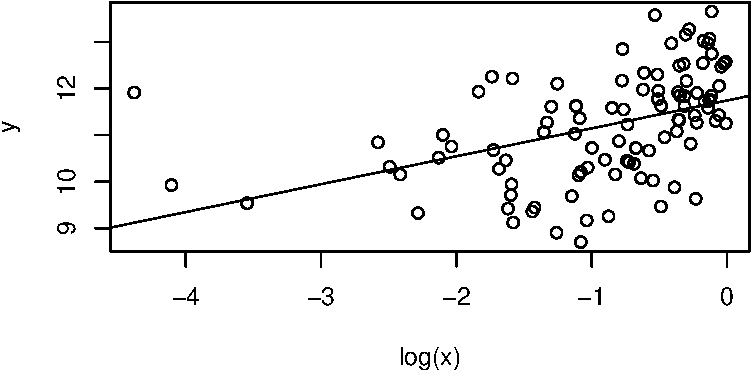
\includegraphics{07-regression1_files/figure-pdf/unnamed-chunk-21-1.pdf}

被説明変数を対数変換する場合も同様に, \texttt{lm} 関数の式の中で
\texttt{log} 関数を使用する. この場合, 係数 \(\beta\) は \(x\)
が1単位変化したときの \(y\) の変化率 (\%) の近似値を表す.

\begin{Shaded}
\begin{Highlighting}[]
\NormalTok{fm }\OtherTok{\textless{}{-}} \FunctionTok{lm}\NormalTok{(}\FunctionTok{log}\NormalTok{(y)}\SpecialCharTok{\textasciitilde{}}\NormalTok{x,}\AttributeTok{data=}\NormalTok{df)}
\FunctionTok{summary}\NormalTok{(fm)}
\DocumentationTok{\#\# }
\DocumentationTok{\#\# Call:}
\DocumentationTok{\#\# lm(formula = log(y) \textasciitilde{} x, data = df)}
\DocumentationTok{\#\# }
\DocumentationTok{\#\# Residuals:}
\DocumentationTok{\#\#       Min        1Q    Median        3Q       Max }
\DocumentationTok{\#\# {-}0.210763 {-}0.055551  0.000211  0.063315  0.182570 }
\DocumentationTok{\#\# }
\DocumentationTok{\#\# Coefficients:}
\DocumentationTok{\#\#             Estimate Std. Error t value Pr(\textgreater{}|t|)    }
\DocumentationTok{\#\# (Intercept)  2.30450    0.01869 123.324  \textless{} 2e{-}16 ***}
\DocumentationTok{\#\# x            0.20660    0.03202   6.453  4.2e{-}09 ***}
\DocumentationTok{\#\# {-}{-}{-}}
\DocumentationTok{\#\# Signif. codes:  0 \textquotesingle{}***\textquotesingle{} 0.001 \textquotesingle{}**\textquotesingle{} 0.01 \textquotesingle{}*\textquotesingle{} 0.05 \textquotesingle{}.\textquotesingle{} 0.1 \textquotesingle{} \textquotesingle{} 1}
\DocumentationTok{\#\# }
\DocumentationTok{\#\# Residual standard error: 0.0883 on 98 degrees of freedom}
\DocumentationTok{\#\# Multiple R{-}squared:  0.2982, Adjusted R{-}squared:  0.291 }
\DocumentationTok{\#\# F{-}statistic: 41.64 on 1 and 98 DF,  p{-}value: 4.197e{-}09}
\end{Highlighting}
\end{Shaded}

散布図と回帰直線を描くと以下のようになる. 縦軸が対数変換された \(y\)
になっている点に注意.

\begin{Shaded}
\begin{Highlighting}[]
\FunctionTok{plot}\NormalTok{(}\FunctionTok{log}\NormalTok{(y)}\SpecialCharTok{\textasciitilde{}}\NormalTok{x,}\AttributeTok{data=}\NormalTok{df)}
\FunctionTok{abline}\NormalTok{(fm)}
\end{Highlighting}
\end{Shaded}

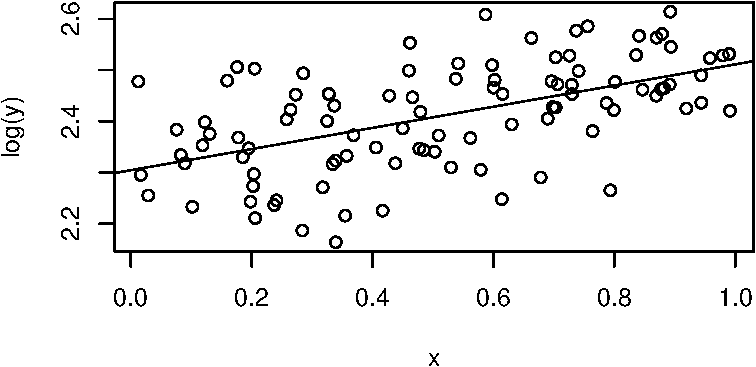
\includegraphics{07-regression1_files/figure-pdf/unnamed-chunk-23-1.pdf}

被説明変数と説明変数の両方を対数変換する場合 (対数線形モデル)
は以下のようにする. この場合, 係数 \(\beta\) は弾力性を表し, \(x\)
が1\%変化したときの \(y\) の変化率 (\%) を表す.

\begin{Shaded}
\begin{Highlighting}[]
\NormalTok{fm }\OtherTok{\textless{}{-}} \FunctionTok{lm}\NormalTok{(}\FunctionTok{log}\NormalTok{(y)}\SpecialCharTok{\textasciitilde{}}\FunctionTok{log}\NormalTok{(x),}\AttributeTok{data=}\NormalTok{df)}
\FunctionTok{summary}\NormalTok{(fm)}
\DocumentationTok{\#\# }
\DocumentationTok{\#\# Call:}
\DocumentationTok{\#\# lm(formula = log(y) \textasciitilde{} log(x), data = df)}
\DocumentationTok{\#\# }
\DocumentationTok{\#\# Residuals:}
\DocumentationTok{\#\#      Min       1Q   Median       3Q      Max }
\DocumentationTok{\#\# {-}0.23737 {-}0.06254  0.01046  0.06266  0.25437 }
\DocumentationTok{\#\# }
\DocumentationTok{\#\# Coefficients:}
\DocumentationTok{\#\#             Estimate Std. Error t value Pr(\textgreater{}|t|)    }
\DocumentationTok{\#\# (Intercept)  2.45945    0.01393 176.574  \textless{} 2e{-}16 ***}
\DocumentationTok{\#\# log(x)       0.05389    0.01128   4.776 6.27e{-}06 ***}
\DocumentationTok{\#\# {-}{-}{-}}
\DocumentationTok{\#\# Signif. codes:  0 \textquotesingle{}***\textquotesingle{} 0.001 \textquotesingle{}**\textquotesingle{} 0.01 \textquotesingle{}*\textquotesingle{} 0.05 \textquotesingle{}.\textquotesingle{} 0.1 \textquotesingle{} \textquotesingle{} 1}
\DocumentationTok{\#\# }
\DocumentationTok{\#\# Residual standard error: 0.09493 on 98 degrees of freedom}
\DocumentationTok{\#\# Multiple R{-}squared:  0.1888, Adjusted R{-}squared:  0.1805 }
\DocumentationTok{\#\# F{-}statistic: 22.81 on 1 and 98 DF,  p{-}value: 6.272e{-}06}
\end{Highlighting}
\end{Shaded}

散布図と回帰直線を描くと以下のようになる.
両軸とも対数変換されている点に注意.

\begin{Shaded}
\begin{Highlighting}[]
\FunctionTok{plot}\NormalTok{(}\FunctionTok{log}\NormalTok{(y)}\SpecialCharTok{\textasciitilde{}}\FunctionTok{log}\NormalTok{(x),}\AttributeTok{data=}\NormalTok{df)}
\FunctionTok{abline}\NormalTok{(fm)}
\end{Highlighting}
\end{Shaded}

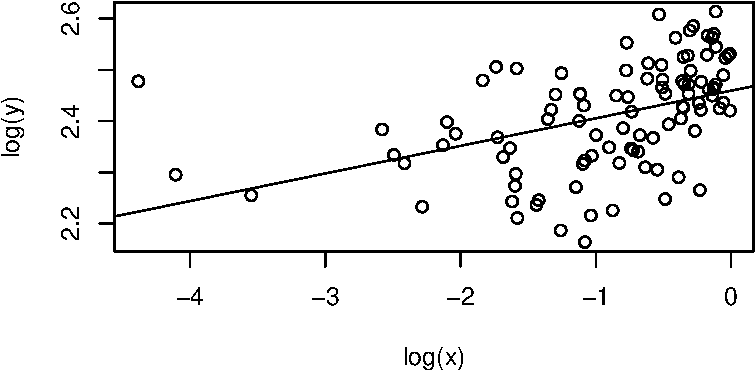
\includegraphics{07-regression1_files/figure-pdf/unnamed-chunk-25-1.pdf}

\subsection{切片なし回帰モデル}\label{ux5207ux7247ux306aux3057ux56deux5e30ux30e2ux30c7ux30eb}

次のモデルを考える. \[
y = \beta x + u
\]

切片を含まないモデルを推定したい場合は, 式の中に \texttt{-1} を加える.
これにより切片項が除外され, 原点を通る回帰直線が推定される.

\begin{Shaded}
\begin{Highlighting}[]
\NormalTok{fm }\OtherTok{\textless{}{-}} \FunctionTok{lm}\NormalTok{(y}\SpecialCharTok{\textasciitilde{}}\NormalTok{x}\DecValTok{{-}1}\NormalTok{,}\AttributeTok{data=}\NormalTok{df)}
\FunctionTok{summary}\NormalTok{(fm)}
\DocumentationTok{\#\# }
\DocumentationTok{\#\# Call:}
\DocumentationTok{\#\# lm(formula = y \textasciitilde{} x {-} 1, data = df)}
\DocumentationTok{\#\# }
\DocumentationTok{\#\# Residuals:}
\DocumentationTok{\#\#    Min     1Q Median     3Q    Max }
\DocumentationTok{\#\# {-}6.027 {-}1.130  2.064  5.628 11.696 }
\DocumentationTok{\#\# }
\DocumentationTok{\#\# Coefficients:}
\DocumentationTok{\#\#   Estimate Std. Error t value Pr(\textgreater{}|t|)    }
\DocumentationTok{\#\# x  17.4286     0.8322   20.94   \textless{}2e{-}16 ***}
\DocumentationTok{\#\# {-}{-}{-}}
\DocumentationTok{\#\# Signif. codes:  0 \textquotesingle{}***\textquotesingle{} 0.001 \textquotesingle{}**\textquotesingle{} 0.01 \textquotesingle{}*\textquotesingle{} 0.05 \textquotesingle{}.\textquotesingle{} 0.1 \textquotesingle{} \textquotesingle{} 1}
\DocumentationTok{\#\# }
\DocumentationTok{\#\# Residual standard error: 4.857 on 99 degrees of freedom}
\DocumentationTok{\#\# Multiple R{-}squared:  0.8159, Adjusted R{-}squared:  0.814 }
\DocumentationTok{\#\# F{-}statistic: 438.6 on 1 and 99 DF,  p{-}value: \textless{} 2.2e{-}16}
\end{Highlighting}
\end{Shaded}

\texttt{+0} を加えても同じ効果が得られる。

\begin{Shaded}
\begin{Highlighting}[]
\NormalTok{fm }\OtherTok{\textless{}{-}} \FunctionTok{lm}\NormalTok{(y}\SpecialCharTok{\textasciitilde{}}\NormalTok{x}\SpecialCharTok{+}\DecValTok{0}\NormalTok{,}\AttributeTok{data=}\NormalTok{df)}
\FunctionTok{summary}\NormalTok{(fm)}
\DocumentationTok{\#\# }
\DocumentationTok{\#\# Call:}
\DocumentationTok{\#\# lm(formula = y \textasciitilde{} x + 0, data = df)}
\DocumentationTok{\#\# }
\DocumentationTok{\#\# Residuals:}
\DocumentationTok{\#\#    Min     1Q Median     3Q    Max }
\DocumentationTok{\#\# {-}6.027 {-}1.130  2.064  5.628 11.696 }
\DocumentationTok{\#\# }
\DocumentationTok{\#\# Coefficients:}
\DocumentationTok{\#\#   Estimate Std. Error t value Pr(\textgreater{}|t|)    }
\DocumentationTok{\#\# x  17.4286     0.8322   20.94   \textless{}2e{-}16 ***}
\DocumentationTok{\#\# {-}{-}{-}}
\DocumentationTok{\#\# Signif. codes:  0 \textquotesingle{}***\textquotesingle{} 0.001 \textquotesingle{}**\textquotesingle{} 0.01 \textquotesingle{}*\textquotesingle{} 0.05 \textquotesingle{}.\textquotesingle{} 0.1 \textquotesingle{} \textquotesingle{} 1}
\DocumentationTok{\#\# }
\DocumentationTok{\#\# Residual standard error: 4.857 on 99 degrees of freedom}
\DocumentationTok{\#\# Multiple R{-}squared:  0.8159, Adjusted R{-}squared:  0.814 }
\DocumentationTok{\#\# F{-}statistic: 438.6 on 1 and 99 DF,  p{-}value: \textless{} 2.2e{-}16}
\end{Highlighting}
\end{Shaded}

\section{重回帰モデル}\label{ux91cdux56deux5e30ux30e2ux30c7ux30eb}

説明変数として \(w\) を加えたモデルを考える. \[
y = \alpha + \beta x +\gamma w+ u
\]

暗黙に以下の仮定を置く。

\begin{itemize}
\tightlist
\item
  \((w_i, x_i,y_i)\) は独立同一分布にしたがう.
\item
  誤差項の期待値はゼロである. \(E[u_i]=0\) である.
\item
  誤差項 \(u_i\) は説明変数 \((x_i, w_i)\) に対して独立である.
\item
  誤差項 \(u_i\) は正規分布にしたがう.
\item
  説明変数間に多重共線性は存在しない. つまり \(x_i\) は \(w_i\)
  の一次変換で表せない.
\end{itemize}

以降ではシミュレーションデータを用いて具体的に確認する。
標本サイズを100とし, 説明変数 \(x\) は0から1の一様分布から, \(w\)
は「H」と「T」からランダムに生成する. 被説明変数 \(y\) は, 真の切片を10,
\(x\) の係数を2, \(w\) が「H」のときに1を加算し,
正規分布の誤差項を加えて生成する.

\begin{Shaded}
\begin{Highlighting}[]
\NormalTok{N }\OtherTok{\textless{}{-}} \DecValTok{100}
\NormalTok{x}\OtherTok{\textless{}{-}}\FunctionTok{runif}\NormalTok{(N)}
\NormalTok{w}\OtherTok{\textless{}{-}}\FunctionTok{sample}\NormalTok{(}\FunctionTok{c}\NormalTok{(}\StringTok{"H"}\NormalTok{,}\StringTok{"T"}\NormalTok{),N,}\AttributeTok{replace=}\ConstantTok{TRUE}\NormalTok{)}
\NormalTok{y }\OtherTok{\textless{}{-}} \DecValTok{10} \SpecialCharTok{+} \DecValTok{2}\SpecialCharTok{*}\NormalTok{x }\SpecialCharTok{+} \FunctionTok{ifelse}\NormalTok{(w}\SpecialCharTok{==}\StringTok{"H"}\NormalTok{,}\DecValTok{1}\NormalTok{,}\DecValTok{0}\NormalTok{) }\SpecialCharTok{+} \FunctionTok{rnorm}\NormalTok{(N)}
\NormalTok{df }\OtherTok{\textless{}{-}} \FunctionTok{data.frame}\NormalTok{(w,x,y)}
\end{Highlighting}
\end{Shaded}

複数の説明変数を含むモデルを推定するには, \texttt{+}
記号で変数を連結する. 式 \texttt{y\textasciitilde{}x+w} は被説明変数
\(y\) を説明変数 \(x\) と \(w\) で回帰することを意味する.

\begin{Shaded}
\begin{Highlighting}[]
\NormalTok{fm }\OtherTok{\textless{}{-}} \FunctionTok{lm}\NormalTok{(y}\SpecialCharTok{\textasciitilde{}}\NormalTok{x}\SpecialCharTok{+}\NormalTok{w,}\AttributeTok{data=}\NormalTok{df)}
\FunctionTok{summary}\NormalTok{(fm)}
\DocumentationTok{\#\# }
\DocumentationTok{\#\# Call:}
\DocumentationTok{\#\# lm(formula = y \textasciitilde{} x + w, data = df)}
\DocumentationTok{\#\# }
\DocumentationTok{\#\# Residuals:}
\DocumentationTok{\#\#      Min       1Q   Median       3Q      Max }
\DocumentationTok{\#\# {-}1.75850 {-}0.64135 {-}0.00448  0.58491  2.79614 }
\DocumentationTok{\#\# }
\DocumentationTok{\#\# Coefficients:}
\DocumentationTok{\#\#             Estimate Std. Error t value Pr(\textgreater{}|t|)    }
\DocumentationTok{\#\# (Intercept)  11.1295     0.2380  46.772  \textless{} 2e{-}16 ***}
\DocumentationTok{\#\# x             1.9331     0.3527   5.481 3.35e{-}07 ***}
\DocumentationTok{\#\# wT           {-}1.1429     0.1995  {-}5.729 1.13e{-}07 ***}
\DocumentationTok{\#\# {-}{-}{-}}
\DocumentationTok{\#\# Signif. codes:  0 \textquotesingle{}***\textquotesingle{} 0.001 \textquotesingle{}**\textquotesingle{} 0.01 \textquotesingle{}*\textquotesingle{} 0.05 \textquotesingle{}.\textquotesingle{} 0.1 \textquotesingle{} \textquotesingle{} 1}
\DocumentationTok{\#\# }
\DocumentationTok{\#\# Residual standard error: 0.997 on 97 degrees of freedom}
\DocumentationTok{\#\# Multiple R{-}squared:  0.3988, Adjusted R{-}squared:  0.3864 }
\DocumentationTok{\#\# F{-}statistic: 32.17 on 2 and 97 DF,  p{-}value: 1.919e{-}11}
\end{Highlighting}
\end{Shaded}

R の特徴として, 因子型 (factor) やカテゴリカル変数 (文字列)
を特に変換することなく自動的にダミー変数として扱える. ここでは \(w\)
が「H」と「T」の2値をとるが, 自動的に一方 (「H」)
のダミー変数が作成され, 「T」が基準カテゴリとなる.

\subsection{自乗項}\label{ux81eaux4e57ux9805}

説明変数として自乗項を加えたモデルを考える. \[
y = \alpha + \beta x + \gamma x^2 + u
\]

自乗項を含めるときは \texttt{I(x\^{}2)} のように \texttt{I()} で囲む。
これは \texttt{\^{}}
が式中で特別扱いされるため、通常の演算として解釈させる工夫である。

\begin{Shaded}
\begin{Highlighting}[]
\NormalTok{fm }\OtherTok{\textless{}{-}} \FunctionTok{lm}\NormalTok{(y}\SpecialCharTok{\textasciitilde{}}\NormalTok{x}\SpecialCharTok{+}\FunctionTok{I}\NormalTok{(x}\SpecialCharTok{\^{}}\DecValTok{2}\NormalTok{),}\AttributeTok{data=}\NormalTok{df)}
\FunctionTok{summary}\NormalTok{(fm)}
\DocumentationTok{\#\# }
\DocumentationTok{\#\# Call:}
\DocumentationTok{\#\# lm(formula = y \textasciitilde{} x + I(x\^{}2), data = df)}
\DocumentationTok{\#\# }
\DocumentationTok{\#\# Residuals:}
\DocumentationTok{\#\#     Min      1Q  Median      3Q     Max }
\DocumentationTok{\#\# {-}2.2424 {-}0.7562  0.0151  0.7145  3.4329 }
\DocumentationTok{\#\# }
\DocumentationTok{\#\# Coefficients:}
\DocumentationTok{\#\#             Estimate Std. Error t value Pr(\textgreater{}|t|)    }
\DocumentationTok{\#\# (Intercept)  10.1529     0.4216  24.083   \textless{}2e{-}16 ***}
\DocumentationTok{\#\# x             4.0102     1.8183   2.205   0.0298 *  }
\DocumentationTok{\#\# I(x\^{}2)       {-}1.8979     1.6566  {-}1.146   0.2548    }
\DocumentationTok{\#\# {-}{-}{-}}
\DocumentationTok{\#\# Signif. codes:  0 \textquotesingle{}***\textquotesingle{} 0.001 \textquotesingle{}**\textquotesingle{} 0.01 \textquotesingle{}*\textquotesingle{} 0.05 \textquotesingle{}.\textquotesingle{} 0.1 \textquotesingle{} \textquotesingle{} 1}
\DocumentationTok{\#\# }
\DocumentationTok{\#\# Residual standard error: 1.146 on 97 degrees of freedom}
\DocumentationTok{\#\# Multiple R{-}squared:  0.2061, Adjusted R{-}squared:  0.1897 }
\DocumentationTok{\#\# F{-}statistic: 12.59 on 2 and 97 DF,  p{-}value: 1.377e{-}05}
\end{Highlighting}
\end{Shaded}

\subsection{交差項}\label{ux4ea4ux5deeux9805}

説明変数として交差項 (interaction term) を加えたモデルを考える. \[
y = \alpha + \beta x + \gamma w + \delta xw + u
\]

交差項(interaction)は \texttt{:} を使って \texttt{x:w} と表記する。
このモデルでは主効果 \texttt{x} と \texttt{w} に加えて, 交差項
\texttt{x:w} を明示的に指定している.

\begin{Shaded}
\begin{Highlighting}[]
\NormalTok{fm}\OtherTok{\textless{}{-}}\FunctionTok{lm}\NormalTok{(y}\SpecialCharTok{\textasciitilde{}}\NormalTok{x}\SpecialCharTok{+}\NormalTok{w}\SpecialCharTok{+}\NormalTok{x}\SpecialCharTok{:}\NormalTok{w,}\AttributeTok{data=}\NormalTok{df)}
\FunctionTok{summary}\NormalTok{(fm)}
\DocumentationTok{\#\# }
\DocumentationTok{\#\# Call:}
\DocumentationTok{\#\# lm(formula = y \textasciitilde{} x + w + x:w, data = df)}
\DocumentationTok{\#\# }
\DocumentationTok{\#\# Residuals:}
\DocumentationTok{\#\#     Min      1Q  Median      3Q     Max }
\DocumentationTok{\#\# {-}1.7795 {-}0.6415 {-}0.0197  0.6003  2.7746 }
\DocumentationTok{\#\# }
\DocumentationTok{\#\# Coefficients:}
\DocumentationTok{\#\#             Estimate Std. Error t value Pr(\textgreater{}|t|)    }
\DocumentationTok{\#\# (Intercept)  11.0956     0.3173  34.972  \textless{} 2e{-}16 ***}
\DocumentationTok{\#\# x             1.9950     0.5208   3.830 0.000228 ***}
\DocumentationTok{\#\# wT           {-}1.0806     0.4333  {-}2.494 0.014346 *  }
\DocumentationTok{\#\# x:wT         {-}0.1153     0.7109  {-}0.162 0.871468    }
\DocumentationTok{\#\# {-}{-}{-}}
\DocumentationTok{\#\# Signif. codes:  0 \textquotesingle{}***\textquotesingle{} 0.001 \textquotesingle{}**\textquotesingle{} 0.01 \textquotesingle{}*\textquotesingle{} 0.05 \textquotesingle{}.\textquotesingle{} 0.1 \textquotesingle{} \textquotesingle{} 1}
\DocumentationTok{\#\# }
\DocumentationTok{\#\# Residual standard error: 1.002 on 96 degrees of freedom}
\DocumentationTok{\#\# Multiple R{-}squared:  0.3989, Adjusted R{-}squared:  0.3802 }
\DocumentationTok{\#\# F{-}statistic: 21.24 on 3 and 96 DF,  p{-}value: 1.234e{-}10}
\end{Highlighting}
\end{Shaded}

\texttt{*} を使えば主要効果と交差項をまとめて指定できる。 \texttt{x*w}
は自動的に \texttt{x\ +\ w\ +\ x:w} に展開される.

\begin{Shaded}
\begin{Highlighting}[]
\NormalTok{fm }\OtherTok{\textless{}{-}} \FunctionTok{lm}\NormalTok{(y}\SpecialCharTok{\textasciitilde{}}\NormalTok{x}\SpecialCharTok{*}\NormalTok{w,}\AttributeTok{data=}\NormalTok{df)}
\FunctionTok{summary}\NormalTok{(fm)}
\DocumentationTok{\#\# }
\DocumentationTok{\#\# Call:}
\DocumentationTok{\#\# lm(formula = y \textasciitilde{} x * w, data = df)}
\DocumentationTok{\#\# }
\DocumentationTok{\#\# Residuals:}
\DocumentationTok{\#\#     Min      1Q  Median      3Q     Max }
\DocumentationTok{\#\# {-}1.7795 {-}0.6415 {-}0.0197  0.6003  2.7746 }
\DocumentationTok{\#\# }
\DocumentationTok{\#\# Coefficients:}
\DocumentationTok{\#\#             Estimate Std. Error t value Pr(\textgreater{}|t|)    }
\DocumentationTok{\#\# (Intercept)  11.0956     0.3173  34.972  \textless{} 2e{-}16 ***}
\DocumentationTok{\#\# x             1.9950     0.5208   3.830 0.000228 ***}
\DocumentationTok{\#\# wT           {-}1.0806     0.4333  {-}2.494 0.014346 *  }
\DocumentationTok{\#\# x:wT         {-}0.1153     0.7109  {-}0.162 0.871468    }
\DocumentationTok{\#\# {-}{-}{-}}
\DocumentationTok{\#\# Signif. codes:  0 \textquotesingle{}***\textquotesingle{} 0.001 \textquotesingle{}**\textquotesingle{} 0.01 \textquotesingle{}*\textquotesingle{} 0.05 \textquotesingle{}.\textquotesingle{} 0.1 \textquotesingle{} \textquotesingle{} 1}
\DocumentationTok{\#\# }
\DocumentationTok{\#\# Residual standard error: 1.002 on 96 degrees of freedom}
\DocumentationTok{\#\# Multiple R{-}squared:  0.3989, Adjusted R{-}squared:  0.3802 }
\DocumentationTok{\#\# F{-}statistic: 21.24 on 3 and 96 DF,  p{-}value: 1.234e{-}10}
\end{Highlighting}
\end{Shaded}

\subsection{エフ検定}\label{ux30a8ux30d5ux691cux5b9a}

今, 帰無仮説が \[
y = \alpha + \beta x + u
\] で, 対立仮説が \[
y = \alpha + \beta x + \gamma w + \delta xw + u
\] となる検定を実施したい.

これは複数の係数(ここでは \(\gamma\) と
\(\delta\))が同時にゼロかどうかを調べる F 検定である。
制約付き検定は、制約のあるモデル(帰無仮説)とないモデル(対立仮説)の残差自乗和を比較することで実施できる。
対立仮説(制約なしモデル)の残差自乗和を \(SSR\)、自由度を \(df\)
とする。 自由度は観測数から推定されるパラメータの数 (説明変数の数と切片)
を減じた数である. 帰無仮説(制約付きモデル)の残差自乗和を
\(SSR_0\)、制約の数を \(q\) とする。
制約の数は帰無仮説の自由度から対立仮説の自由度を差し引いた数である.
このとき, 以下のF値は帰無仮説が正しいもとで自由度 \((q, df)\)
のF分布にしたがう. \[
F = \frac{(SSR_0-SSR)/q}{SSR/df}
\]

R でF値を手動で計算するには以下のようにする. まず両方のモデルを推定し,
それぞれの自由度 (\texttt{\$df}) と残差自乗和 (\texttt{deviance})
を取り出す. 制約の数 \(q\) は両モデルの自由度の差である.
F値は上記の式に従って計算する.

\begin{Shaded}
\begin{Highlighting}[]
\NormalTok{fm0 }\OtherTok{\textless{}{-}} \FunctionTok{lm}\NormalTok{(y}\SpecialCharTok{\textasciitilde{}}\NormalTok{x,}\AttributeTok{data=}\NormalTok{df)}
\NormalTok{fm1 }\OtherTok{\textless{}{-}} \FunctionTok{lm}\NormalTok{(y}\SpecialCharTok{\textasciitilde{}}\NormalTok{x}\SpecialCharTok{*}\NormalTok{w,}\AttributeTok{data=}\NormalTok{df)}
\NormalTok{dof }\OtherTok{\textless{}{-}}\NormalTok{ fm1}\SpecialCharTok{$}\NormalTok{df}
\NormalTok{q }\OtherTok{\textless{}{-}}\NormalTok{ fm0}\SpecialCharTok{$}\NormalTok{df}\SpecialCharTok{{-}}\NormalTok{dof}
\NormalTok{SSR0 }\OtherTok{\textless{}{-}} \FunctionTok{deviance}\NormalTok{(fm0)}
\NormalTok{SSR }\OtherTok{\textless{}{-}} \FunctionTok{deviance}\NormalTok{(fm1)}
\NormalTok{(F }\OtherTok{\textless{}{-}}\NormalTok{ ((SSR0}\SpecialCharTok{{-}}\NormalTok{SSR)}\SpecialCharTok{/}\NormalTok{q)}\SpecialCharTok{/}\NormalTok{(SSR}\SpecialCharTok{/}\NormalTok{dof))}
\DocumentationTok{\#\# [1] 16.25963}
\end{Highlighting}
\end{Shaded}

F 値に対する p 値は \texttt{pf()} で計算できる。 \texttt{pf()} は F
分布の累積分布関数で、\texttt{1\ -\ pf(F,\ df1,\ df2)} が上側確率(p
値)となる。 第一自由度 (\texttt{df1}) は制約の数 \(q\), 第二自由度
(\texttt{df2}) は対立仮説の自由度である.

\begin{Shaded}
\begin{Highlighting}[]
\DecValTok{1}\SpecialCharTok{{-}}\FunctionTok{pf}\NormalTok{(F,}\AttributeTok{df1=}\NormalTok{q,}\AttributeTok{df2=}\NormalTok{dof)}
\DocumentationTok{\#\# [1] 8.289809e{-}07}
\end{Highlighting}
\end{Shaded}

これらの手順は \texttt{anova()} を使えば自動で計算できる。
\texttt{anova} 関数に2つのモデルを渡すと, 自動的にエフ検定を実施し,
F値とp値を表示してくれる.

\begin{Shaded}
\begin{Highlighting}[]
\FunctionTok{anova}\NormalTok{(fm0,fm1)}
\DocumentationTok{\#\# Analysis of Variance Table}
\DocumentationTok{\#\# }
\DocumentationTok{\#\# Model 1: y \textasciitilde{} x}
\DocumentationTok{\#\# Model 2: y \textasciitilde{} x * w}
\DocumentationTok{\#\#   Res.Df     RSS Df Sum of Sq     F   Pr(\textgreater{}F)    }
\DocumentationTok{\#\# 1     98 129.039                                }
\DocumentationTok{\#\# 2     96  96.388  2    32.651 16.26 8.29e{-}07 ***}
\DocumentationTok{\#\# {-}{-}{-}}
\DocumentationTok{\#\# Signif. codes:  0 \textquotesingle{}***\textquotesingle{} 0.001 \textquotesingle{}**\textquotesingle{} 0.01 \textquotesingle{}*\textquotesingle{} 0.05 \textquotesingle{}.\textquotesingle{} 0.1 \textquotesingle{} \textquotesingle{} 1}
\end{Highlighting}
\end{Shaded}

モデルの順序を入れ替えても検定統計量や p 値に変わりはない。
ただし残差自乗和の差の符号が変わるため、出力の一部が入れ替わって見える。

\begin{Shaded}
\begin{Highlighting}[]
\FunctionTok{anova}\NormalTok{(fm1,fm0)}
\DocumentationTok{\#\# Analysis of Variance Table}
\DocumentationTok{\#\# }
\DocumentationTok{\#\# Model 1: y \textasciitilde{} x * w}
\DocumentationTok{\#\# Model 2: y \textasciitilde{} x}
\DocumentationTok{\#\#   Res.Df     RSS Df Sum of Sq     F   Pr(\textgreater{}F)    }
\DocumentationTok{\#\# 1     96  96.388                                }
\DocumentationTok{\#\# 2     98 129.039 {-}2   {-}32.651 16.26 8.29e{-}07 ***}
\DocumentationTok{\#\# {-}{-}{-}}
\DocumentationTok{\#\# Signif. codes:  0 \textquotesingle{}***\textquotesingle{} 0.001 \textquotesingle{}**\textquotesingle{} 0.01 \textquotesingle{}*\textquotesingle{} 0.05 \textquotesingle{}.\textquotesingle{} 0.1 \textquotesingle{} \textquotesingle{} 1}
\end{Highlighting}
\end{Shaded}

\bookmarksetup{startatroot}

\chapter{現代的仮定のもとでの最小二乗法}\label{ux73feux4ee3ux7684ux4eeeux5b9aux306eux3082ux3068ux3067ux306eux6700ux5c0fux4e8cux4e57ux6cd5}

\begin{Shaded}
\begin{Highlighting}[]
\FunctionTok{library}\NormalTok{(AER)}
\FunctionTok{library}\NormalTok{(estimatr)}
\end{Highlighting}
\end{Shaded}

前節において以下の仮定を置いていた.

\begin{itemize}
\tightlist
\item
  \((x_i,y_i)\) は独立同一分布にしたがう.
\item
  \(E[u_i]=0\) である.
\item
  \(u_i\) と \(x_i\) は独立である.
\item
  \(u_i\) は正規分布にしたがう.
\end{itemize}

これらの仮定を緩めることで分析にどのような影響をあたえるのかを見ていく.

仮想的に以下のモデルを考える.

\begin{Shaded}
\begin{Highlighting}[]
\NormalTok{N }\OtherTok{\textless{}{-}} \DecValTok{100}
\NormalTok{x}\OtherTok{\textless{}{-}}\FunctionTok{runif}\NormalTok{(N)}
\NormalTok{w}\OtherTok{\textless{}{-}}\FunctionTok{sample}\NormalTok{(}\FunctionTok{c}\NormalTok{(}\StringTok{"H"}\NormalTok{,}\StringTok{"T"}\NormalTok{),N,}\AttributeTok{replace=}\ConstantTok{TRUE}\NormalTok{)}
\NormalTok{y }\OtherTok{\textless{}{-}} \DecValTok{10} \SpecialCharTok{+} \DecValTok{2}\SpecialCharTok{*}\NormalTok{x }\SpecialCharTok{+} \FunctionTok{ifelse}\NormalTok{(w}\SpecialCharTok{==}\StringTok{"H"}\NormalTok{,}\DecValTok{1}\NormalTok{,}\DecValTok{0}\NormalTok{) }\SpecialCharTok{+} \FunctionTok{rnorm}\NormalTok{(N)}
\NormalTok{df }\OtherTok{\textless{}{-}} \FunctionTok{data.frame}\NormalTok{(w,x,y)}
\end{Highlighting}
\end{Shaded}

作図すると以下である.

\begin{Shaded}
\begin{Highlighting}[]
\FunctionTok{plot}\NormalTok{(y}\SpecialCharTok{\textasciitilde{}}\NormalTok{x)}
\end{Highlighting}
\end{Shaded}

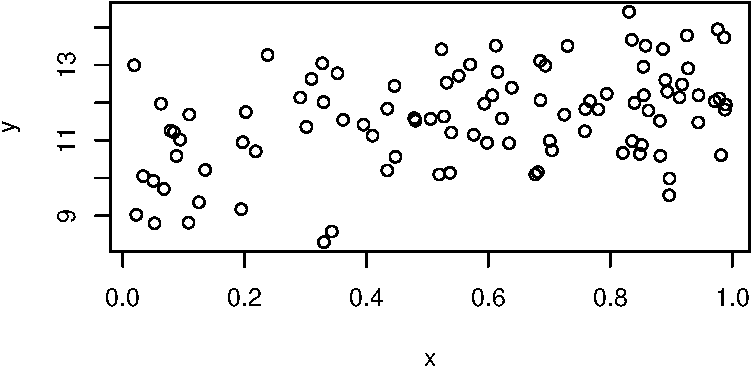
\includegraphics{08-regression2_files/figure-pdf/unnamed-chunk-3-1.pdf}

\section{正規性の仮定について}\label{ux6b63ux898fux6027ux306eux4eeeux5b9aux306bux3064ux3044ux3066}

十分な観測値が得られるばあい, \(u_i\)
が正規分布にしたがっていないくても, 中心極限定理定理より,
最小二乗法推定量は正規分布に近似できる.

ここの係数ゼロのティー検定について, ライブラリ \texttt{AER} を導入して
\texttt{coeftest} を用いればよい. まず \texttt{lm}
コマンドを用いて2つのモデルを推定する. \texttt{fm1} は説明変数
\texttt{x} とダミー変数 \texttt{w} およびそれらの交差項を含むモデル,
\texttt{fm0} は \texttt{x} のみを含むモデルである.

\begin{Shaded}
\begin{Highlighting}[]
\NormalTok{fm1 }\OtherTok{\textless{}{-}} \FunctionTok{lm}\NormalTok{(y}\SpecialCharTok{\textasciitilde{}}\NormalTok{x}\SpecialCharTok{*}\NormalTok{w,}\AttributeTok{data=}\NormalTok{df)}
\NormalTok{fm0 }\OtherTok{\textless{}{-}} \FunctionTok{lm}\NormalTok{(y}\SpecialCharTok{\textasciitilde{}}\NormalTok{x,}\AttributeTok{data=}\NormalTok{df)}
\FunctionTok{coeftest}\NormalTok{(fm1,}\AttributeTok{df=}\ConstantTok{Inf}\NormalTok{)}
\DocumentationTok{\#\# }
\DocumentationTok{\#\# z test of coefficients:}
\DocumentationTok{\#\# }
\DocumentationTok{\#\#             Estimate Std. Error z value  Pr(\textgreater{}|z|)    }
\DocumentationTok{\#\# (Intercept) 11.36728    0.34034 33.4002 \textless{} 2.2e{-}16 ***}
\DocumentationTok{\#\# x            1.63777    0.53571  3.0572  0.002234 ** }
\DocumentationTok{\#\# wT          {-}1.43560    0.45021 {-}3.1887  0.001429 ** }
\DocumentationTok{\#\# x:wT         0.35775    0.70184  0.5097  0.610241    }
\DocumentationTok{\#\# {-}{-}{-}}
\DocumentationTok{\#\# Signif. codes:  0 \textquotesingle{}***\textquotesingle{} 0.001 \textquotesingle{}**\textquotesingle{} 0.01 \textquotesingle{}*\textquotesingle{} 0.05 \textquotesingle{}.\textquotesingle{} 0.1 \textquotesingle{} \textquotesingle{} 1}
\end{Highlighting}
\end{Shaded}

\texttt{coeftest} コマンドは係数の検定を実行する関数である. オプション
\texttt{df=Inf} を指定すると,
ティー分布の代わりに標準正規分布(自由度無限大のティー分布)を用いた検定を実行する.
これは大標本のもとでの漸近的な検定である.
ただ十分なデータのもとではティー値のままでもよい.

同様に複数制約の場合, エフ検定統計量に制約の数を乗じた統計量が
自由度が制約数のカイ二乗分布にしたがうことが知られている. これをR
で実施するには \texttt{waldtest} を用いればよい. \texttt{waldtest}
コマンドは制約のあるモデル(\texttt{fm0})と制約のないモデル(\texttt{fm1})を比較して,
複数の係数がゼロかどうかを検定する関数である.

\begin{Shaded}
\begin{Highlighting}[]
\FunctionTok{waldtest}\NormalTok{(fm0,fm1,}\AttributeTok{test=}\StringTok{"Chisq"}\NormalTok{)}
\DocumentationTok{\#\# Wald test}
\DocumentationTok{\#\# }
\DocumentationTok{\#\# Model 1: y \textasciitilde{} x}
\DocumentationTok{\#\# Model 2: y \textasciitilde{} x * w}
\DocumentationTok{\#\#   Res.Df Df  Chisq Pr(\textgreater{}Chisq)    }
\DocumentationTok{\#\# 1     98                         }
\DocumentationTok{\#\# 2     96  2 34.955  2.568e{-}08 ***}
\DocumentationTok{\#\# {-}{-}{-}}
\DocumentationTok{\#\# Signif. codes:  0 \textquotesingle{}***\textquotesingle{} 0.001 \textquotesingle{}**\textquotesingle{} 0.01 \textquotesingle{}*\textquotesingle{} 0.05 \textquotesingle{}.\textquotesingle{} 0.1 \textquotesingle{} \textquotesingle{} 1}
\end{Highlighting}
\end{Shaded}

オプション \texttt{test="Chisq"} を指定すると,
エフ検定統計量に制約の数を乗じた統計量が自由度が制約数のカイ二乗分布にしたがうことを利用した検定を実行する.
これは大標本での漸近的な検定である.

エフ検定も十分なデータのもとではそのままでよいであろう.

オプション \texttt{test} を付けなければエフ検定を実施する.

\begin{Shaded}
\begin{Highlighting}[]
\FunctionTok{waldtest}\NormalTok{(fm0,fm1)}
\DocumentationTok{\#\# Wald test}
\DocumentationTok{\#\# }
\DocumentationTok{\#\# Model 1: y \textasciitilde{} x}
\DocumentationTok{\#\# Model 2: y \textasciitilde{} x * w}
\DocumentationTok{\#\#   Res.Df Df      F    Pr(\textgreater{}F)    }
\DocumentationTok{\#\# 1     98                        }
\DocumentationTok{\#\# 2     96  2 17.478 3.366e{-}07 ***}
\DocumentationTok{\#\# {-}{-}{-}}
\DocumentationTok{\#\# Signif. codes:  0 \textquotesingle{}***\textquotesingle{} 0.001 \textquotesingle{}**\textquotesingle{} 0.01 \textquotesingle{}*\textquotesingle{} 0.05 \textquotesingle{}.\textquotesingle{} 0.1 \textquotesingle{} \textquotesingle{} 1}
\end{Highlighting}
\end{Shaded}

この結果はエフ統計量とそのP値を表示している.

これは \texttt{anova} コマンドと同じである.

\begin{Shaded}
\begin{Highlighting}[]
\FunctionTok{anova}\NormalTok{(fm0,fm1)}
\DocumentationTok{\#\# Analysis of Variance Table}
\DocumentationTok{\#\# }
\DocumentationTok{\#\# Model 1: y \textasciitilde{} x}
\DocumentationTok{\#\# Model 2: y \textasciitilde{} x * w}
\DocumentationTok{\#\#   Res.Df    RSS Df Sum of Sq      F    Pr(\textgreater{}F)    }
\DocumentationTok{\#\# 1     98 139.55                                  }
\DocumentationTok{\#\# 2     96 102.30  2     37.25 17.478 3.366e{-}07 ***}
\DocumentationTok{\#\# {-}{-}{-}}
\DocumentationTok{\#\# Signif. codes:  0 \textquotesingle{}***\textquotesingle{} 0.001 \textquotesingle{}**\textquotesingle{} 0.01 \textquotesingle{}*\textquotesingle{} 0.05 \textquotesingle{}.\textquotesingle{} 0.1 \textquotesingle{} \textquotesingle{} 1}
\end{Highlighting}
\end{Shaded}

\texttt{anova} コマンドも2つのモデルを比較してエフ検定を実行する.

複数制約の検定としてLM検定というのもある. 制約付きの回帰分析を実行し,
その残差を制約なしのモデルの説明変数に回帰する.
その決定係数に観測数を掛けた統計量が自由どが制約の数のカイ二乗分布にしたがうことが知られている.

以下ではLM検定統計量を手動で計算している.

\begin{Shaded}
\begin{Highlighting}[]
\NormalTok{lmt }\OtherTok{\textless{}{-}} \FunctionTok{lm}\NormalTok{(}\FunctionTok{I}\NormalTok{(}\FunctionTok{resid}\NormalTok{(fm1))}\SpecialCharTok{\textasciitilde{}}\NormalTok{w}\SpecialCharTok{*}\NormalTok{x,}\AttributeTok{data=}\NormalTok{df)}
\NormalTok{(lmt }\OtherTok{\textless{}{-}} \FunctionTok{nrow}\NormalTok{(df)}\SpecialCharTok{*}\FunctionTok{summary}\NormalTok{(lmt)}\SpecialCharTok{$}\NormalTok{r.squared)}
\DocumentationTok{\#\# [1] 1.334534e{-}29}
\DecValTok{1}\SpecialCharTok{{-}}\FunctionTok{pchisq}\NormalTok{(lmt,}\AttributeTok{df=}\DecValTok{1}\NormalTok{)}
\DocumentationTok{\#\# [1] 1}
\end{Highlighting}
\end{Shaded}

最初の行では, \texttt{fm1}
の残差(\texttt{resid(fm1)})を被説明変数とし, \texttt{w*x}
を説明変数として回帰分析を実行している. 2行目では,
その決定係数(\texttt{summary(lmt)\$r.squared})に観測数(\texttt{nrow(df)})を掛けてLM検定統計量を計算している.
3行目では, \texttt{pchisq}
コマンドを用いて自由度1のカイ二乗分布のもとでP値を計算している.

\section{誤差項と説明変数が独立の仮定について}\label{ux8aa4ux5deeux9805ux3068ux8aacux660eux5909ux6570ux304cux72ecux7acbux306eux4eeeux5b9aux306bux3064ux3044ux3066}

また \(u_i\) と \(x_i\) は独立でなく, \(u_i\) と \(x_i\)
が無相関という弱い条件のもとでも, 一致推定量であることが知られている.
ただ不偏推定量は保証できない. また
線形推定量のなかで最小の分散とも言えない.\footnote{正確にいえば,
  不偏推定量のとめには条件付き期待値が説明変数に依存しないことが必要である.
  また線形推定量のなかで最小の分散になるためには
  条件付き分散が説明変数に依存しないことが必要である.}
また独立のときの標準誤差の推定量が一致推定量でない.

ただし,
別の分散のもとで正規分布に近似できることがしられている.\footnote{正確には観測される変数に4次のモーメントが存在するという仮定が必要となる.
  この仮定の直感的な意味は異常値が存在しないことである.} つまり,
説明変数と誤差項が無相関であるが, 独立とまでは言い切れない場合,
最小二乗推定量を実行した際, 別の方法で分散を推定する必要がある.
この別の分散をロバスト分散という.

R でロバスト分散を推定するにはパッケージ \texttt{AER}
を導入するのが簡単である. 次のコマンド \texttt{coeftest}
を実行すればよい.

\begin{Shaded}
\begin{Highlighting}[]
\FunctionTok{coeftest}\NormalTok{(fm1,}\AttributeTok{vcov=}\NormalTok{vcovHC)}
\DocumentationTok{\#\# }
\DocumentationTok{\#\# t test of coefficients:}
\DocumentationTok{\#\# }
\DocumentationTok{\#\#             Estimate Std. Error t value  Pr(\textgreater{}|t|)    }
\DocumentationTok{\#\# (Intercept) 11.36728    0.37192 30.5639 \textless{} 2.2e{-}16 ***}
\DocumentationTok{\#\# x            1.63777    0.57410  2.8528  0.005308 ** }
\DocumentationTok{\#\# wT          {-}1.43560    0.49379 {-}2.9073  0.004527 ** }
\DocumentationTok{\#\# x:wT         0.35775    0.74834  0.4781  0.633697    }
\DocumentationTok{\#\# {-}{-}{-}}
\DocumentationTok{\#\# Signif. codes:  0 \textquotesingle{}***\textquotesingle{} 0.001 \textquotesingle{}**\textquotesingle{} 0.01 \textquotesingle{}*\textquotesingle{} 0.05 \textquotesingle{}.\textquotesingle{} 0.1 \textquotesingle{} \textquotesingle{} 1}
\end{Highlighting}
\end{Shaded}

\texttt{coeftest} コマンドのオプション \texttt{vcov=vcovHC}
を指定することで,
不均一分散に頑健な(heteroskedasticity-consistent)標準誤差を用いた検定が実行される.
\texttt{vcovHC} は分散共分散行列をロバスト推定する関数である.

先の値と標準誤差が違っていることが確認できるであろう. ただこの値は STATA
と少し異なっている. STATA と同じにするには

\begin{Shaded}
\begin{Highlighting}[]
\FunctionTok{coeftest}\NormalTok{(fm1,}\AttributeTok{vcov=}\FunctionTok{vcovHC}\NormalTok{(fm1,}\AttributeTok{type=}\StringTok{"HC1"}\NormalTok{))}
\DocumentationTok{\#\# }
\DocumentationTok{\#\# t test of coefficients:}
\DocumentationTok{\#\# }
\DocumentationTok{\#\#             Estimate Std. Error t value  Pr(\textgreater{}|t|)    }
\DocumentationTok{\#\# (Intercept) 11.36728    0.35147 32.3425 \textless{} 2.2e{-}16 ***}
\DocumentationTok{\#\# x            1.63777    0.54368  3.0124  0.003314 ** }
\DocumentationTok{\#\# wT          {-}1.43560    0.47193 {-}3.0420  0.003031 ** }
\DocumentationTok{\#\# x:wT         0.35775    0.71615  0.4995  0.618535    }
\DocumentationTok{\#\# {-}{-}{-}}
\DocumentationTok{\#\# Signif. codes:  0 \textquotesingle{}***\textquotesingle{} 0.001 \textquotesingle{}**\textquotesingle{} 0.01 \textquotesingle{}*\textquotesingle{} 0.05 \textquotesingle{}.\textquotesingle{} 0.1 \textquotesingle{} \textquotesingle{} 1}
\end{Highlighting}
\end{Shaded}

としなければならない. オプション \texttt{type="HC1"}
は小標本補正を施したロバスト分散推定量を指定している.
これはSTATAのデフォルト設定と同じである.

またティー分布でなく正規分布とすることもできる.

\begin{Shaded}
\begin{Highlighting}[]
\FunctionTok{coeftest}\NormalTok{(fm0,}\AttributeTok{vcov=}\NormalTok{vcovHC,}\AttributeTok{df=}\ConstantTok{Inf}\NormalTok{)}
\DocumentationTok{\#\# }
\DocumentationTok{\#\# z test of coefficients:}
\DocumentationTok{\#\# }
\DocumentationTok{\#\#             Estimate Std. Error z value  Pr(\textgreater{}|z|)    }
\DocumentationTok{\#\# (Intercept) 10.56579    0.28536  37.026 \textless{} 2.2e{-}16 ***}
\DocumentationTok{\#\# x            1.79305    0.42793   4.190 2.789e{-}05 ***}
\DocumentationTok{\#\# {-}{-}{-}}
\DocumentationTok{\#\# Signif. codes:  0 \textquotesingle{}***\textquotesingle{} 0.001 \textquotesingle{}**\textquotesingle{} 0.01 \textquotesingle{}*\textquotesingle{} 0.05 \textquotesingle{}.\textquotesingle{} 0.1 \textquotesingle{} \textquotesingle{} 1}
\end{Highlighting}
\end{Shaded}

オプション \texttt{df=Inf} を追加することで,
標準正規分布を用いた検定を実行する.

複数の係数についての検定は \texttt{waldtest} を実行すればよい.

\begin{Shaded}
\begin{Highlighting}[]
\FunctionTok{waldtest}\NormalTok{(fm0,fm1,}\AttributeTok{vcov=}\NormalTok{vcovHC)}
\DocumentationTok{\#\# Wald test}
\DocumentationTok{\#\# }
\DocumentationTok{\#\# Model 1: y \textasciitilde{} x}
\DocumentationTok{\#\# Model 2: y \textasciitilde{} x * w}
\DocumentationTok{\#\#   Res.Df Df      F    Pr(\textgreater{}F)    }
\DocumentationTok{\#\# 1     98                        }
\DocumentationTok{\#\# 2     96  2 16.754 5.737e{-}07 ***}
\DocumentationTok{\#\# {-}{-}{-}}
\DocumentationTok{\#\# Signif. codes:  0 \textquotesingle{}***\textquotesingle{} 0.001 \textquotesingle{}**\textquotesingle{} 0.01 \textquotesingle{}*\textquotesingle{} 0.05 \textquotesingle{}.\textquotesingle{} 0.1 \textquotesingle{} \textquotesingle{} 1}
\end{Highlighting}
\end{Shaded}

オプション \texttt{vcov=vcovHC} を指定することで,
ロバスト分散を用いたワルド検定を実行する.

先の結果はエフ検定であるが,
カイ二乗検定を実施するには以下を実施すればよい.

\begin{Shaded}
\begin{Highlighting}[]
\FunctionTok{waldtest}\NormalTok{(fm0,fm1,}\AttributeTok{vcov=}\NormalTok{vcovHC, }\AttributeTok{test=}\StringTok{"Chisq"}\NormalTok{)}
\DocumentationTok{\#\# Wald test}
\DocumentationTok{\#\# }
\DocumentationTok{\#\# Model 1: y \textasciitilde{} x}
\DocumentationTok{\#\# Model 2: y \textasciitilde{} x * w}
\DocumentationTok{\#\#   Res.Df Df  Chisq Pr(\textgreater{}Chisq)    }
\DocumentationTok{\#\# 1     98                         }
\DocumentationTok{\#\# 2     96  2 33.509  5.293e{-}08 ***}
\DocumentationTok{\#\# {-}{-}{-}}
\DocumentationTok{\#\# Signif. codes:  0 \textquotesingle{}***\textquotesingle{} 0.001 \textquotesingle{}**\textquotesingle{} 0.01 \textquotesingle{}*\textquotesingle{} 0.05 \textquotesingle{}.\textquotesingle{} 0.1 \textquotesingle{} \textquotesingle{} 1}
\end{Highlighting}
\end{Shaded}

オプション \texttt{test="Chisq"} を追加することで,
エフ統計量の代わりにカイ二乗統計量を用いた検定を実行する.

最近開発されたパッケージ
\texttt{estimatr}のコマンド \texttt{lm\_robust} を用いるとロバスト分散のもとの推定値が簡単に計算できる.

\begin{Shaded}
\begin{Highlighting}[]
\NormalTok{fm2}\OtherTok{\textless{}{-}} \FunctionTok{lm\_robust}\NormalTok{(y}\SpecialCharTok{\textasciitilde{}}\NormalTok{x}\SpecialCharTok{*}\NormalTok{w,}\AttributeTok{data=}\NormalTok{df)}
\FunctionTok{summary}\NormalTok{(fm2)}
\DocumentationTok{\#\# }
\DocumentationTok{\#\# Call:}
\DocumentationTok{\#\# lm\_robust(formula = y \textasciitilde{} x * w, data = df)}
\DocumentationTok{\#\# }
\DocumentationTok{\#\# Standard error type:  HC2 }
\DocumentationTok{\#\# }
\DocumentationTok{\#\# Coefficients:}
\DocumentationTok{\#\#             Estimate Std. Error t value  Pr(\textgreater{}|t|) CI Lower CI Upper DF}
\DocumentationTok{\#\# (Intercept)  11.3673     0.3578 31.7700 9.779e{-}53  10.6571  12.0775 96}
\DocumentationTok{\#\# x             1.6378     0.5529  2.9621 3.852e{-}03   0.5402   2.7353 96}
\DocumentationTok{\#\# wT           {-}1.4356     0.4777 {-}3.0050 3.388e{-}03  {-}2.3839  {-}0.4873 96}
\DocumentationTok{\#\# x:wT          0.3578     0.7245  0.4938 6.226e{-}01  {-}1.0804   1.7959 96}
\DocumentationTok{\#\# }
\DocumentationTok{\#\# Multiple R{-}squared:  0.3917 ,    Adjusted R{-}squared:  0.3727 }
\DocumentationTok{\#\# F{-}statistic: 19.69 on 3 and 96 DF,  p{-}value: 4.998e{-}10}
\end{Highlighting}
\end{Shaded}

\texttt{lm\_robust} コマンドは回帰分析を実行し,
デフォルトでロバスト標準誤差を計算する. これにより \texttt{lm} と
\texttt{coeftest} を別々に実行する手間が省ける.

オプション \texttt{se\_type\ =\ "stata"}
を用いればSTATAと同じ計算が可能である.

また以下のオプションをつければ分散均一の場合も計算できる.

\begin{Shaded}
\begin{Highlighting}[]
\NormalTok{fm3}\OtherTok{\textless{}{-}} \FunctionTok{lm\_robust}\NormalTok{(y}\SpecialCharTok{\textasciitilde{}}\NormalTok{x}\SpecialCharTok{*}\NormalTok{w,}\AttributeTok{data=}\NormalTok{df,}\AttributeTok{se\_type =} \StringTok{"classical"}\NormalTok{)}
\FunctionTok{summary}\NormalTok{(fm3)}
\DocumentationTok{\#\# }
\DocumentationTok{\#\# Call:}
\DocumentationTok{\#\# lm\_robust(formula = y \textasciitilde{} x * w, data = df, se\_type = "classical")}
\DocumentationTok{\#\# }
\DocumentationTok{\#\# Standard error type:  classical }
\DocumentationTok{\#\# }
\DocumentationTok{\#\# Coefficients:}
\DocumentationTok{\#\#             Estimate Std. Error t value  Pr(\textgreater{}|t|) CI Lower CI Upper DF}
\DocumentationTok{\#\# (Intercept)  11.3673     0.3403 33.4002 1.190e{-}54  10.6917  12.0428 96}
\DocumentationTok{\#\# x             1.6378     0.5357  3.0572 2.894e{-}03   0.5744   2.7011 96}
\DocumentationTok{\#\# wT           {-}1.4356     0.4502 {-}3.1887 1.930e{-}03  {-}2.3293  {-}0.5419 96}
\DocumentationTok{\#\# x:wT          0.3578     0.7018  0.5097 6.114e{-}01  {-}1.0354   1.7509 96}
\DocumentationTok{\#\# }
\DocumentationTok{\#\# Multiple R{-}squared:  0.3917 ,    Adjusted R{-}squared:  0.3727 }
\DocumentationTok{\#\# F{-}statistic:  20.6 on 3 and 96 DF,  p{-}value: 2.176e{-}10}
\end{Highlighting}
\end{Shaded}

オプション \texttt{se\_type\ =\ "classical"} を指定すると,
通常の(ロバストでない)標準誤差を計算する. これは \texttt{lm}
コマンドの結果と同じである.

\section{分散均一の検定}\label{ux5206ux6563ux5747ux4e00ux306eux691cux5b9a}

誤差項が説明変数と独立のときと無相関のときでは標準誤差の推定量が異なる.
正確にいうと,
条件付き分散が説明変数に依存するかどうかによって標準誤差の推定量が異なる.
このことは分散均一と呼ばれている.

誤差項の分散が均一かどうかは検定可能である. 有名な検定方法としてBP
(Breusch-Pagan) 検定というものがある. BP検定は帰無仮説が分散均一で,
対立仮説が分散が説明変数と線形関係になっている場合の検定である.

残差の自乗を被説明変数として回帰分析をおこない,
その決定係数に観測数をかけたものが検定統計量となる.
以下ではBP検定統計量を手動で計算している.

\begin{Shaded}
\begin{Highlighting}[]
\NormalTok{bpt }\OtherTok{\textless{}{-}} \FunctionTok{lm}\NormalTok{(}\FunctionTok{I}\NormalTok{(}\FunctionTok{resid}\NormalTok{(fm1)}\SpecialCharTok{\^{}}\DecValTok{2}\NormalTok{)}\SpecialCharTok{\textasciitilde{}}\NormalTok{w}\SpecialCharTok{*}\NormalTok{x,}\AttributeTok{data=}\NormalTok{df)}
\NormalTok{(bpt }\OtherTok{\textless{}{-}}\FunctionTok{nrow}\NormalTok{(df)}\SpecialCharTok{*}\FunctionTok{summary}\NormalTok{(bpt)}\SpecialCharTok{$}\NormalTok{r.squared)}
\DocumentationTok{\#\# [1] 0.831414}
\DecValTok{1}\SpecialCharTok{{-}}\FunctionTok{pchisq}\NormalTok{(bpt,}\AttributeTok{df=}\DecValTok{3}\NormalTok{)}
\DocumentationTok{\#\# [1] 0.8419394}
\end{Highlighting}
\end{Shaded}

最初の行では, \texttt{fm1}
の残差の二乗(\texttt{resid(fm1)\^{}2})を被説明変数とし, \texttt{w*x}
を説明変数として回帰分析を実行している. \texttt{I()} 関数は,
数式内で算術演算を実行するために用いる. 2行目では,
その決定係数に観測数を掛けてBP検定統計量を計算している. 3行目では,
自由度3(説明変数の数)のカイ二乗分布のもとでP値を計算している.

ここでの例ではP値が5\%を超えているので帰無仮説を棄却できないので,
分散均一を仮定してよいことが示唆されている.

R では \texttt{bptest} コマンドを用いて簡単にBP検定を実施できる.

\begin{Shaded}
\begin{Highlighting}[]
\FunctionTok{bptest}\NormalTok{(fm1)}
\DocumentationTok{\#\# }
\DocumentationTok{\#\#  studentized Breusch{-}Pagan test}
\DocumentationTok{\#\# }
\DocumentationTok{\#\# data:  fm1}
\DocumentationTok{\#\# BP = 0.83141, df = 3, p{-}value = 0.8419}
\end{Highlighting}
\end{Shaded}

\texttt{bptest} コマンドは自動的にBP検定統計量とP値を計算してくれる.

これまでのBPテストは誤差項の分散が説明変数の線形関係あることを暗黙に仮定している.
非線形性を考慮するために説明変数の二次項を導入した分散不均一性の検定をホワイト検定という.
説明変数が複数ある場合ホワイト検定は煩雑になるため,
被説明変数の予測値を使って計算することがある.
そのときホワイトテストは以下で実施する.

\begin{Shaded}
\begin{Highlighting}[]
\NormalTok{wht }\OtherTok{\textless{}{-}} \FunctionTok{lm}\NormalTok{(}\FunctionTok{I}\NormalTok{(}\FunctionTok{resid}\NormalTok{(fm1)}\SpecialCharTok{\^{}}\DecValTok{2}\NormalTok{)}\SpecialCharTok{\textasciitilde{}}\FunctionTok{fitted}\NormalTok{(fm1)}\SpecialCharTok{+}\FunctionTok{I}\NormalTok{(}\FunctionTok{fitted}\NormalTok{(fm1)}\SpecialCharTok{\^{}}\DecValTok{2}\NormalTok{),}\AttributeTok{data=}\NormalTok{df)}
\NormalTok{(wht }\OtherTok{\textless{}{-}} \FunctionTok{nrow}\NormalTok{(df)}\SpecialCharTok{*}\FunctionTok{summary}\NormalTok{(wht)}\SpecialCharTok{$}\NormalTok{r.squared)}
\DocumentationTok{\#\# [1] 0.7517355}
\DecValTok{1}\SpecialCharTok{{-}}\FunctionTok{pchisq}\NormalTok{(wht,}\AttributeTok{df=}\DecValTok{2}\NormalTok{)}
\DocumentationTok{\#\# [1] 0.6866931}
\end{Highlighting}
\end{Shaded}

最初の行では, 残差の二乗を被説明変数とし,
予測値(\texttt{fitted(fm1)})とその二乗を説明変数として回帰分析を実行している.
これにより分散の非線形性を検出できる. 2行目では,
その決定係数に観測数を掛けてホワイト検定統計量を計算している. 3行目では,
自由度2のカイ二乗分布のもとでP値を計算している.

ホワイト検定でも分散均一が示唆されている.

もしくは \texttt{bptest}
コマンドに予測値とその二乗を指定して実行することもできる.

\begin{Shaded}
\begin{Highlighting}[]
\FunctionTok{bptest}\NormalTok{(fm1,}\SpecialCharTok{\textasciitilde{}}\FunctionTok{fitted}\NormalTok{(fm1)}\SpecialCharTok{+}\FunctionTok{I}\NormalTok{(}\FunctionTok{fitted}\NormalTok{(fm1)}\SpecialCharTok{\^{}}\DecValTok{2}\NormalTok{))}
\DocumentationTok{\#\# }
\DocumentationTok{\#\#  studentized Breusch{-}Pagan test}
\DocumentationTok{\#\# }
\DocumentationTok{\#\# data:  fm1}
\DocumentationTok{\#\# BP = 0.75174, df = 2, p{-}value = 0.6867}
\end{Highlighting}
\end{Shaded}

このコマンドは上記の手動計算と同じ結果を返す.

このように分散均一性は検定することが可能であるが,
そもそも分散均一が疑われる場合は,
ロバスト分散で推定するので十分であるため最近の実証分析ではこの検定は実施されない.

\bookmarksetup{startatroot}

\chapter{操作変数法}\label{ux64cdux4f5cux5909ux6570ux6cd5}

\section{データ}\label{ux30c7ux30fcux30bf}

\begin{Shaded}
\begin{Highlighting}[]
\FunctionTok{library}\NormalTok{(AER)}
\FunctionTok{library}\NormalTok{(wooldridge)}
\FunctionTok{library}\NormalTok{(estimatr)}
\FunctionTok{data}\NormalTok{(}\StringTok{"mroz"}\NormalTok{, }\AttributeTok{package=}\StringTok{"wooldridge"}\NormalTok{)}
\NormalTok{df }\OtherTok{\textless{}{-}} \FunctionTok{subset}\NormalTok{(mroz, inlf}\SpecialCharTok{==}\DecValTok{1}\NormalTok{)}
\end{Highlighting}
\end{Shaded}

\section{操作変数}\label{ux64cdux4f5cux5909ux6570}

これまで回帰モデルで一致推定量を得るためには次の仮定が必要であった.

\begin{enumerate}
\def\labelenumi{\arabic{enumi}.}
\tightlist
\item
  母集団が線形モデル
\item
  標本が無作為抽出
\item
  誤差項が平均ゼロで説明変数と無相関
\item
  説明変数に多重共線性が存在しない
\end{enumerate}

3つ目の仮定が必ずしも成立しない場合の推定方法を紹介する.

そのために, 外生変数と内生変数と操作変数の3つの概念を導入する.
誤差項と相関が無い説明変数を \textbf{外生変数} といい,
誤差項と相関がある説明変数を \textbf{内生変数} という. \textbf{操作変数}
とは, 説明変数に含まれず, 説明変数と相関をもち,
誤差項と相関をもたない変数のことである.
なお操作変数の個数は内生変数の個数より多苦なければならない。

R においては \texttt{ivreg} コマンドを用いて操作変数法を実行する.
このコマンドは \texttt{AER} パッケージに含まれており, 基本的な書式は
\texttt{ivreg(被説明変数\ \textasciitilde{}\ 内生変数\ \textbar{}\ 操作変数,\ data=データフレーム)}
である. ここで被説明変数は \texttt{log(wage)}, 内生変数は \texttt{educ},
操作変数は \texttt{fatheduc} である.

以下のコマンドで操作変数法を実行し, \texttt{coef}
コマンドで推定された係数を取り出す.

\begin{Shaded}
\begin{Highlighting}[]
\NormalTok{fm  }\OtherTok{\textless{}{-}} \FunctionTok{ivreg}\NormalTok{(}\FunctionTok{log}\NormalTok{(wage)}\SpecialCharTok{\textasciitilde{}}\NormalTok{educ}\SpecialCharTok{|}\NormalTok{fatheduc, }\AttributeTok{data=}\NormalTok{df)}
\FunctionTok{coef}\NormalTok{(fm)}
\DocumentationTok{\#\# (Intercept)        educ }
\DocumentationTok{\#\#  0.44110339  0.05917348}
\end{Highlighting}
\end{Shaded}

傾きの推定値は操作変数推定量の公式を用いて直接計算することもできる.
具体的には,
被説明変数と操作変数の共分散を内生変数と操作変数の共分散で割ることで得られる.
以下のコマンドで \texttt{cov} 関数を用いて共分散を計算し,
同じ推定値が得られることを確認する.

\begin{Shaded}
\begin{Highlighting}[]
\FunctionTok{with}\NormalTok{(df, }\FunctionTok{cov}\NormalTok{(}\FunctionTok{log}\NormalTok{(wage),fatheduc)}\SpecialCharTok{/}\FunctionTok{cov}\NormalTok{(educ,fatheduc))}
\DocumentationTok{\#\# [1] 0.05917348}
\end{Highlighting}
\end{Shaded}

\section{2段階最小二乗法}\label{ux6bb5ux968eux6700ux5c0fux4e8cux4e57ux6cd5}

複数の説明変数あり, 操作変数の数が内生変数の数以上のとき,
係数の一致推定量を得るには二段階最小自乗法を用いる.
二段階最小二乗法は次の手順で実行される:

\begin{enumerate}
\def\labelenumi{\arabic{enumi}.}
\tightlist
\item
  それぞれの内生変数を外生変数と操作変数に回帰させて, その予測値を得る.
\item
  被説明変数を外生変数と内生変数の予測値に回帰させて, その係数を得る.
\end{enumerate}

この係数が一致推定量になるための条件は以下である.

\begin{itemize}
\tightlist
\item
  母集団が線形モデル
\item
  標本が無作為抽出
\item
  誤差項が平均ゼロで操作変数と外生変数に対して独立.
\item
  操作変数は内生変数と相関をもつ.
\item
  外生変数と内生変数の予測値に多重共線性が存在しない`
\end{itemize}

R においては \texttt{ivreg} コマンドを用いて二段階最小二乗法を実行する.
複数の説明変数がある場合の書式は
\texttt{ivreg(被説明変数\ \textasciitilde{}\ 内生変数\ +\ 外生変数\ \textbar{}\ 外生変数\ +\ 操作変数,\ data=データフレーム)}
である. ここで被説明変数は \texttt{log(wage)}, 内生変数は \texttt{educ},
外生変数は \texttt{exper}, \texttt{I(exper\^{}2)}, 操作変数は
\texttt{motheduc}, \texttt{fatheduc} である. 注意点として, パイプ記号
\texttt{\textbar{}} の右側には外生変数も含める必要がある.

以下のコマンドで二段階最小二乗法を実行し, \texttt{summary}
コマンドで推定結果の要約を表示する.

\begin{Shaded}
\begin{Highlighting}[]
\NormalTok{fm  }\OtherTok{\textless{}{-}} \FunctionTok{ivreg}\NormalTok{(}\FunctionTok{log}\NormalTok{(wage)}\SpecialCharTok{\textasciitilde{}}\NormalTok{educ}\SpecialCharTok{+}\NormalTok{exper}\SpecialCharTok{+}\FunctionTok{I}\NormalTok{(exper}\SpecialCharTok{\^{}}\DecValTok{2}\NormalTok{)}\SpecialCharTok{|}
\NormalTok{            exper}\SpecialCharTok{+}\FunctionTok{I}\NormalTok{(exper}\SpecialCharTok{\^{}}\DecValTok{2}\NormalTok{)}\SpecialCharTok{+}\NormalTok{motheduc}\SpecialCharTok{+}\NormalTok{fatheduc,}
            \AttributeTok{data=}\NormalTok{df)}
\FunctionTok{summary}\NormalTok{(fm)}
\DocumentationTok{\#\# }
\DocumentationTok{\#\# Call:}
\DocumentationTok{\#\# ivreg(formula = log(wage) \textasciitilde{} educ + exper + I(exper\^{}2) | exper + }
\DocumentationTok{\#\#     I(exper\^{}2) + motheduc + fatheduc, data = df)}
\DocumentationTok{\#\# }
\DocumentationTok{\#\# Residuals:}
\DocumentationTok{\#\#     Min      1Q  Median      3Q     Max }
\DocumentationTok{\#\# {-}3.0986 {-}0.3196  0.0551  0.3689  2.3493 }
\DocumentationTok{\#\# }
\DocumentationTok{\#\# Coefficients:}
\DocumentationTok{\#\#               Estimate Std. Error t value Pr(\textgreater{}|t|)   }
\DocumentationTok{\#\# (Intercept)  0.0481003  0.4003281   0.120  0.90442   }
\DocumentationTok{\#\# educ         0.0613966  0.0314367   1.953  0.05147 . }
\DocumentationTok{\#\# exper        0.0441704  0.0134325   3.288  0.00109 **}
\DocumentationTok{\#\# I(exper\^{}2)  {-}0.0008990  0.0004017  {-}2.238  0.02574 * }
\DocumentationTok{\#\# {-}{-}{-}}
\DocumentationTok{\#\# Signif. codes:  0 \textquotesingle{}***\textquotesingle{} 0.001 \textquotesingle{}**\textquotesingle{} 0.01 \textquotesingle{}*\textquotesingle{} 0.05 \textquotesingle{}.\textquotesingle{} 0.1 \textquotesingle{} \textquotesingle{} 1}
\DocumentationTok{\#\# }
\DocumentationTok{\#\# Residual standard error: 0.6747 on 424 degrees of freedom}
\DocumentationTok{\#\# Multiple R{-}Squared: 0.1357,  Adjusted R{-}squared: 0.1296 }
\DocumentationTok{\#\# Wald test: 8.141 on 3 and 424 DF,  p{-}value: 2.787e{-}05}
\end{Highlighting}
\end{Shaded}

二段階最小二乗法の手順を \texttt{lm} コマンドを用いて手動で実行し,
同じ係数推定値が得られることを確認できる.
ただし標準誤差の値が異なっている.
なぜなら残差は内生変数および外生変数から算出させる必要があるが,
以下のやりかただと内生変数の予測値および外生変数から算出するためである.

以下では第一段階として \texttt{lm} コマンドで内生変数 \texttt{educ}
を外生変数と操作変数に回帰し, \texttt{fitted}
コマンドで予測値を取得する.
第二段階として被説明変数を外生変数と内生変数の予測値に回帰する.

\begin{Shaded}
\begin{Highlighting}[]
\NormalTok{ols1 }\OtherTok{\textless{}{-}} \FunctionTok{lm}\NormalTok{(educ}\SpecialCharTok{\textasciitilde{}}\NormalTok{exper}\SpecialCharTok{+}\FunctionTok{I}\NormalTok{(exper}\SpecialCharTok{\^{}}\DecValTok{2}\NormalTok{)}\SpecialCharTok{+}\NormalTok{motheduc}\SpecialCharTok{+}\NormalTok{fatheduc,  }\AttributeTok{data =}\NormalTok{ df)}
\NormalTok{ols2 }\OtherTok{\textless{}{-}} \FunctionTok{lm}\NormalTok{(}\FunctionTok{log}\NormalTok{(wage)}\SpecialCharTok{\textasciitilde{}}\FunctionTok{fitted}\NormalTok{(ols1)}\SpecialCharTok{+}\NormalTok{exper}\SpecialCharTok{+}\FunctionTok{I}\NormalTok{(exper}\SpecialCharTok{\^{}}\DecValTok{2}\NormalTok{),  }\AttributeTok{data =}\NormalTok{ df)}
\FunctionTok{summary}\NormalTok{(ols2)}
\DocumentationTok{\#\# }
\DocumentationTok{\#\# Call:}
\DocumentationTok{\#\# lm(formula = log(wage) \textasciitilde{} fitted(ols1) + exper + I(exper\^{}2), data = df)}
\DocumentationTok{\#\# }
\DocumentationTok{\#\# Residuals:}
\DocumentationTok{\#\#     Min      1Q  Median      3Q     Max }
\DocumentationTok{\#\# {-}3.1631 {-}0.3539  0.0326  0.3818  2.3727 }
\DocumentationTok{\#\# }
\DocumentationTok{\#\# Coefficients:}
\DocumentationTok{\#\#                Estimate Std. Error t value Pr(\textgreater{}|t|)   }
\DocumentationTok{\#\# (Intercept)   0.0481003  0.4197565   0.115  0.90882   }
\DocumentationTok{\#\# fitted(ols1)  0.0613966  0.0329624   1.863  0.06321 . }
\DocumentationTok{\#\# exper         0.0441704  0.0140844   3.136  0.00183 **}
\DocumentationTok{\#\# I(exper\^{}2)   {-}0.0008990  0.0004212  {-}2.134  0.03338 * }
\DocumentationTok{\#\# {-}{-}{-}}
\DocumentationTok{\#\# Signif. codes:  0 \textquotesingle{}***\textquotesingle{} 0.001 \textquotesingle{}**\textquotesingle{} 0.01 \textquotesingle{}*\textquotesingle{} 0.05 \textquotesingle{}.\textquotesingle{} 0.1 \textquotesingle{} \textquotesingle{} 1}
\DocumentationTok{\#\# }
\DocumentationTok{\#\# Residual standard error: 0.7075 on 424 degrees of freedom}
\DocumentationTok{\#\# Multiple R{-}squared:  0.04978,    Adjusted R{-}squared:  0.04306 }
\DocumentationTok{\#\# F{-}statistic: 7.405 on 3 and 424 DF,  p{-}value: 7.615e{-}05}
\end{Highlighting}
\end{Shaded}

\subsection{複数制約の検定}\label{ux8907ux6570ux5236ux7d04ux306eux691cux5b9a}

帰無仮説が複数の係数制約を課す場合のワルド検定を実施する. 例えば,
2つの外生変数 \texttt{exper} と \texttt{I(exper\^{}2)}
の係数がともにゼロであるという仮説を検定する.

まず \texttt{ivreg}
コマンドで制約モデル(外生変数を含まないモデル)を推定し,
\texttt{waldtest} コマンドで制約なしモデルと比較する. \texttt{waldtest}
コマンドは2つのモデルを引数にとり, ワルド検定を実行する.

\begin{Shaded}
\begin{Highlighting}[]
\NormalTok{fm0 }\OtherTok{\textless{}{-}} \FunctionTok{ivreg}\NormalTok{(}\FunctionTok{log}\NormalTok{(wage)}\SpecialCharTok{\textasciitilde{}}\NormalTok{educ}\SpecialCharTok{|}\NormalTok{motheduc}\SpecialCharTok{+}\NormalTok{fatheduc,}\AttributeTok{data=}\NormalTok{df)}
\FunctionTok{waldtest}\NormalTok{(fm0,fm)}
\DocumentationTok{\#\# Wald test}
\DocumentationTok{\#\# }
\DocumentationTok{\#\# Model 1: log(wage) \textasciitilde{} educ | motheduc + fatheduc}
\DocumentationTok{\#\# Model 2: log(wage) \textasciitilde{} educ + exper + I(exper\^{}2) | exper + I(exper\^{}2) + }
\DocumentationTok{\#\#     motheduc + fatheduc}
\DocumentationTok{\#\#   Res.Df Df  Chisq Pr(\textgreater{}Chisq)    }
\DocumentationTok{\#\# 1    426                         }
\DocumentationTok{\#\# 2    424  2 19.639  5.439e{-}05 ***}
\DocumentationTok{\#\# {-}{-}{-}}
\DocumentationTok{\#\# Signif. codes:  0 \textquotesingle{}***\textquotesingle{} 0.001 \textquotesingle{}**\textquotesingle{} 0.01 \textquotesingle{}*\textquotesingle{} 0.05 \textquotesingle{}.\textquotesingle{} 0.1 \textquotesingle{} \textquotesingle{} 1}
\end{Highlighting}
\end{Shaded}

LM検定(ラグランジュ乗数検定)も実行可能である. まず \texttt{resid}
コマンドで制約モデルの残差を取得し,
その残差を制約される説明変数に回帰する. \texttt{nrow}
コマンドで観測数を取得し, 決定係数 \texttt{r.squared}
を乗じてLM統計量を計算する. 最後に \texttt{pchisq}
コマンドでカイ二乗分布のP値を計算する(自由度は制約の数3).

\begin{Shaded}
\begin{Highlighting}[]
\NormalTok{lmt }\OtherTok{\textless{}{-}} \FunctionTok{lm}\NormalTok{(}\FunctionTok{resid}\NormalTok{(fm0)}\SpecialCharTok{\textasciitilde{}}\NormalTok{educ }\SpecialCharTok{+}\NormalTok{ exper }\SpecialCharTok{+} \FunctionTok{I}\NormalTok{(exper}\SpecialCharTok{\^{}}\DecValTok{2}\NormalTok{) ,}\AttributeTok{data=}\NormalTok{df)}
\NormalTok{(lmt }\OtherTok{\textless{}{-}} \FunctionTok{nrow}\NormalTok{(df)}\SpecialCharTok{*}\FunctionTok{summary}\NormalTok{(lmt)}\SpecialCharTok{$}\NormalTok{r.squared)}
\DocumentationTok{\#\# [1] 33.97987}
\DecValTok{1}\SpecialCharTok{{-}}\FunctionTok{pchisq}\NormalTok{(lmt,}\AttributeTok{df=}\DecValTok{3}\NormalTok{)}
\DocumentationTok{\#\# [1] 2.000665e{-}07}
\end{Highlighting}
\end{Shaded}

\section{特定化検定}\label{ux7279ux5b9aux5316ux691cux5b9a}

操作変数法が妥当かどうかを検証するために, 複数の特定化検定を実施する.
\texttt{summary} コマンドにオプション \texttt{diagnostics\ =\ TRUE}
を追加すると, 弱操作変数検定(Weak instruments), Wu-Hausman検定,
Sargan検定を一度に実行できる. これらの検定結果から, 操作変数の妥当性,
内生性の有無, 操作変数の外生性を確認できる.

\begin{Shaded}
\begin{Highlighting}[]
\FunctionTok{summary}\NormalTok{(fm, }\AttributeTok{diagnostics =} \ConstantTok{TRUE}\NormalTok{)}
\DocumentationTok{\#\# }
\DocumentationTok{\#\# Call:}
\DocumentationTok{\#\# ivreg(formula = log(wage) \textasciitilde{} educ + exper + I(exper\^{}2) | exper + }
\DocumentationTok{\#\#     I(exper\^{}2) + motheduc + fatheduc, data = df)}
\DocumentationTok{\#\# }
\DocumentationTok{\#\# Residuals:}
\DocumentationTok{\#\#     Min      1Q  Median      3Q     Max }
\DocumentationTok{\#\# {-}3.0986 {-}0.3196  0.0551  0.3689  2.3493 }
\DocumentationTok{\#\# }
\DocumentationTok{\#\# Coefficients:}
\DocumentationTok{\#\#               Estimate Std. Error t value Pr(\textgreater{}|t|)   }
\DocumentationTok{\#\# (Intercept)  0.0481003  0.4003281   0.120  0.90442   }
\DocumentationTok{\#\# educ         0.0613966  0.0314367   1.953  0.05147 . }
\DocumentationTok{\#\# exper        0.0441704  0.0134325   3.288  0.00109 **}
\DocumentationTok{\#\# I(exper\^{}2)  {-}0.0008990  0.0004017  {-}2.238  0.02574 * }
\DocumentationTok{\#\# }
\DocumentationTok{\#\# Diagnostic tests:}
\DocumentationTok{\#\#                  df1 df2 statistic p{-}value    }
\DocumentationTok{\#\# Weak instruments   2 423    55.400  \textless{}2e{-}16 ***}
\DocumentationTok{\#\# Wu{-}Hausman         1 423     2.793  0.0954 .  }
\DocumentationTok{\#\# Sargan             1  NA     0.378  0.5386    }
\DocumentationTok{\#\# {-}{-}{-}}
\DocumentationTok{\#\# Signif. codes:  0 \textquotesingle{}***\textquotesingle{} 0.001 \textquotesingle{}**\textquotesingle{} 0.01 \textquotesingle{}*\textquotesingle{} 0.05 \textquotesingle{}.\textquotesingle{} 0.1 \textquotesingle{} \textquotesingle{} 1}
\DocumentationTok{\#\# }
\DocumentationTok{\#\# Residual standard error: 0.6747 on 424 degrees of freedom}
\DocumentationTok{\#\# Multiple R{-}Squared: 0.1357,  Adjusted R{-}squared: 0.1296 }
\DocumentationTok{\#\# Wald test: 8.141 on 3 and 424 DF,  p{-}value: 2.787e{-}05}
\end{Highlighting}
\end{Shaded}

\subsection{Weak instruments}\label{weak-instruments}

操作変数が内生変数と弱い相関関係しかない場合, \textbf{弱操作変数}という.
弱操作変数の場合, 推定量の性質が悪化するため,
操作変数が十分に強い相関を持つかを検定する必要がある.

検定手順は以下の通りである: それぞれの内生変数に対して,
帰無仮説を内生変数を外生変数のみに回帰させたモデルとし,
対立仮説を内生変数を外生変数および操作変数に回帰させたモデルとし,
F検定を実施する.

以下のコマンドで \texttt{lm} による制約モデルを推定し, \texttt{anova}
コマンドで第一段階の回帰モデル \texttt{ols1} と比較してF検定を実行する.
この結果が先の \texttt{diagnostics\ =\ TRUE}
で得られた弱操作変数検定と同じであることを確認されたい.

\begin{Shaded}
\begin{Highlighting}[]
\NormalTok{ols0 }\OtherTok{\textless{}{-}} \FunctionTok{lm}\NormalTok{(educ }\SpecialCharTok{\textasciitilde{}}\NormalTok{ exper }\SpecialCharTok{+} \FunctionTok{I}\NormalTok{(exper}\SpecialCharTok{\^{}}\DecValTok{2}\NormalTok{), }\AttributeTok{data =}\NormalTok{ df)}
\FunctionTok{anova}\NormalTok{(ols0, ols1)}
\DocumentationTok{\#\# Analysis of Variance Table}
\DocumentationTok{\#\# }
\DocumentationTok{\#\# Model 1: educ \textasciitilde{} exper + I(exper\^{}2)}
\DocumentationTok{\#\# Model 2: educ \textasciitilde{} exper + I(exper\^{}2) + motheduc + fatheduc}
\DocumentationTok{\#\#   Res.Df    RSS Df Sum of Sq    F    Pr(\textgreater{}F)    }
\DocumentationTok{\#\# 1    425 2219.2                                }
\DocumentationTok{\#\# 2    423 1758.6  2    460.64 55.4 \textless{} 2.2e{-}16 ***}
\DocumentationTok{\#\# {-}{-}{-}}
\DocumentationTok{\#\# Signif. codes:  0 \textquotesingle{}***\textquotesingle{} 0.001 \textquotesingle{}**\textquotesingle{} 0.01 \textquotesingle{}*\textquotesingle{} 0.05 \textquotesingle{}.\textquotesingle{} 0.1 \textquotesingle{} \textquotesingle{} 1}
\end{Highlighting}
\end{Shaded}

\subsection{Wu-Hausman 検定}\label{wu-hausman-ux691cux5b9a}

Wu-Hausman 検定は 帰無仮説が誤差項と説明変数が無相関,
対立仮説が誤差項と説明変数が相関ありの検定をおこなう.
帰無仮説のもとでは, OLSも2SLSも一致推定量であるが,
OLSの方が効率的である.
よって検定統計量のP値が十分小さいなら帰無仮説は棄却され,
内生性があることになり操作変数法(2SLS)を選択する.
そうでなければより効率的な最小二乗法(OLS)を実施する.

具体的には以下のF検定を実施する:

\begin{enumerate}
\def\labelenumi{\arabic{enumi}.}
\tightlist
\item
  \texttt{lm} コマンドでそれぞれの内生変数を外生変数に回帰し,
  \texttt{resid} コマンドで残差を得る (\texttt{resid(ols1)})
\item
  \texttt{lm} コマンドで被説明変数を説明変数に回帰する (\texttt{ols3})
\item
  \texttt{update}
  コマンドで被説明変数を説明変数および先程の残差に回帰する
  (\texttt{ols4})
\item
  \texttt{anova}
  コマンドでこれらの残差の係数はゼロであるという帰無仮説のもとF検定を実施する
\end{enumerate}

以下のコマンドが先の \texttt{diagnostics\ =\ TRUE}
で得られたWu-Hausman検定と同じであることを確認されたい.

\begin{Shaded}
\begin{Highlighting}[]
\NormalTok{ols3 }\OtherTok{\textless{}{-}} \FunctionTok{lm}\NormalTok{(}\FunctionTok{log}\NormalTok{(wage) }\SpecialCharTok{\textasciitilde{}}\NormalTok{ educ  }\SpecialCharTok{+}\NormalTok{ exper }\SpecialCharTok{+} \FunctionTok{I}\NormalTok{(exper}\SpecialCharTok{\^{}}\DecValTok{2}\NormalTok{), }\AttributeTok{data =}\NormalTok{ df)}
\NormalTok{ols4 }\OtherTok{\textless{}{-}} \FunctionTok{update}\NormalTok{(ols3, . }\SpecialCharTok{\textasciitilde{}}\NormalTok{ . }\SpecialCharTok{+} \FunctionTok{resid}\NormalTok{(ols1))}
\FunctionTok{anova}\NormalTok{(ols3,ols4)}
\DocumentationTok{\#\# Analysis of Variance Table}
\DocumentationTok{\#\# }
\DocumentationTok{\#\# Model 1: log(wage) \textasciitilde{} educ + exper + I(exper\^{}2)}
\DocumentationTok{\#\# Model 2: log(wage) \textasciitilde{} educ + exper + I(exper\^{}2) + resid(ols1)}
\DocumentationTok{\#\#   Res.Df    RSS Df Sum of Sq      F  Pr(\textgreater{}F)  }
\DocumentationTok{\#\# 1    424 188.31                              }
\DocumentationTok{\#\# 2    423 187.07  1     1.235 2.7926 0.09544 .}
\DocumentationTok{\#\# {-}{-}{-}}
\DocumentationTok{\#\# Signif. codes:  0 \textquotesingle{}***\textquotesingle{} 0.001 \textquotesingle{}**\textquotesingle{} 0.01 \textquotesingle{}*\textquotesingle{} 0.05 \textquotesingle{}.\textquotesingle{} 0.1 \textquotesingle{} \textquotesingle{} 1}
\end{Highlighting}
\end{Shaded}

\subsection{Sargan 検定}\label{sargan-ux691cux5b9a}

Sargan 検定は 誤差項が操作変数 (および外生変数)
と相関しているかどうかを検定する.
帰無仮説は操作変数が外生的である(相関が無い)場合で,
対立仮説は操作変数が内生的である(相関がある)場合である.
この検定は操作変数が過剰識別されている(操作変数の数が内生変数の数より多い)場合にのみ実施可能である.

LM検定(ラグランジュ乗数検定)を以下の手順で実施する:

\begin{enumerate}
\def\labelenumi{\arabic{enumi}.}
\tightlist
\item
  \texttt{resid} コマンドで二段階最小二乗法を実施したときの残差を得る
  (\texttt{resid(fm)})
\item
  \texttt{lm} コマンドで残差を外生変数および操作変数に回帰する
\item
  \texttt{nrow} コマンドで観測数を取得し, 回帰の決定係数
  \texttt{r.squared} を乗じたLM統計量を得る
\item
  \texttt{pchisq} コマンドで検定統計量のP値を計算する.
  検定統計量は帰無仮説のもと,
  操作変数の数から内生変数の数を差し引いた自由度(この例では1)のカイ二乗分布にしたがう
\end{enumerate}

以下のコマンドが先の \texttt{diagnostics\ =\ TRUE}
で得られたSargan検定と同じであることを確認されたい.

\begin{Shaded}
\begin{Highlighting}[]
\NormalTok{jt }\OtherTok{\textless{}{-}} \FunctionTok{lm}\NormalTok{(}\FunctionTok{resid}\NormalTok{(fm)}\SpecialCharTok{\textasciitilde{}}\NormalTok{exper}\SpecialCharTok{+}\FunctionTok{I}\NormalTok{(exper}\SpecialCharTok{\^{}}\DecValTok{2}\NormalTok{)}\SpecialCharTok{+}\NormalTok{motheduc}\SpecialCharTok{+}\NormalTok{fatheduc,}\AttributeTok{data=}\NormalTok{df)}
\NormalTok{(jt }\OtherTok{\textless{}{-}} \FunctionTok{nrow}\NormalTok{(df)}\SpecialCharTok{*}\FunctionTok{summary}\NormalTok{(jt)}\SpecialCharTok{$}\NormalTok{r.squared)}
\DocumentationTok{\#\# [1] 0.3780714}
\DecValTok{1}\SpecialCharTok{{-}}\FunctionTok{pchisq}\NormalTok{(jt,}\AttributeTok{df=}\DecValTok{1}\NormalTok{)}
\DocumentationTok{\#\# [1] 0.5386372}
\end{Highlighting}
\end{Shaded}

\section{ロバスト分散}\label{ux30edux30d0ux30b9ux30c8ux5206ux6563}

以上の分析は, 誤差項が操作変数と独立かつ均一分散の場合の分析である.
独立でない場合や分散不均一の場合, 推定量の分散が変わりうる.
そうした場合に頑健な分散推定量を\textbf{ロバスト分散}という.

ロバスト分散にもとづく推定結果を得るには, \texttt{summary}
コマンドにオプション \texttt{vcov\ =\ vcovHC} を追加する.
\texttt{vcovHC} は不均一分散に頑健な分散共分散行列を計算する関数である.
オプション \texttt{df\ =\ Inf} は自由度を無限大とし,
t分布ではなく正規分布を用いて検定を行う.

\begin{Shaded}
\begin{Highlighting}[]
\FunctionTok{summary}\NormalTok{(fm, }\AttributeTok{vcov =}\NormalTok{ vcovHC, }\AttributeTok{df =} \ConstantTok{Inf}\NormalTok{)}
\DocumentationTok{\#\# }
\DocumentationTok{\#\# Call:}
\DocumentationTok{\#\# ivreg(formula = log(wage) \textasciitilde{} educ + exper + I(exper\^{}2) | exper + }
\DocumentationTok{\#\#     I(exper\^{}2) + motheduc + fatheduc, data = df)}
\DocumentationTok{\#\# }
\DocumentationTok{\#\# Residuals:}
\DocumentationTok{\#\#     Min      1Q  Median      3Q     Max }
\DocumentationTok{\#\# {-}3.0986 {-}0.3196  0.0551  0.3689  2.3493 }
\DocumentationTok{\#\# }
\DocumentationTok{\#\# Coefficients:}
\DocumentationTok{\#\#               Estimate Std. Error z value Pr(\textgreater{}|z|)   }
\DocumentationTok{\#\# (Intercept)  0.0481003  0.4337795   0.111  0.91171   }
\DocumentationTok{\#\# educ         0.0613966  0.0336597   1.824  0.06815 . }
\DocumentationTok{\#\# exper        0.0441704  0.0157661   2.802  0.00508 **}
\DocumentationTok{\#\# I(exper\^{}2)  {-}0.0008990  0.0004391  {-}2.047  0.04062 * }
\DocumentationTok{\#\# {-}{-}{-}}
\DocumentationTok{\#\# Signif. codes:  0 \textquotesingle{}***\textquotesingle{} 0.001 \textquotesingle{}**\textquotesingle{} 0.01 \textquotesingle{}*\textquotesingle{} 0.05 \textquotesingle{}.\textquotesingle{} 0.1 \textquotesingle{} \textquotesingle{} 1}
\DocumentationTok{\#\# }
\DocumentationTok{\#\# Residual standard error: 0.6747 on Inf degrees of freedom}
\DocumentationTok{\#\# Multiple R{-}Squared: 0.1357,  Adjusted R{-}squared: 0.1296 }
\DocumentationTok{\#\# Wald test: 18.11 on 3 DF,  p{-}value: 0.0004168}
\end{Highlighting}
\end{Shaded}

係数の検定結果のみを表示したい場合は, \texttt{coeftest}
コマンドを用いる.
このコマンドは推定されたモデルオブジェクトと分散共分散行列を引数にとり,
係数のt検定結果を表示する.

\begin{Shaded}
\begin{Highlighting}[]
\FunctionTok{coeftest}\NormalTok{(fm, }\AttributeTok{vcov=}\NormalTok{vcovHC)}
\DocumentationTok{\#\# }
\DocumentationTok{\#\# t test of coefficients:}
\DocumentationTok{\#\# }
\DocumentationTok{\#\#                Estimate  Std. Error t value Pr(\textgreater{}|t|)   }
\DocumentationTok{\#\# (Intercept)  0.04810030  0.43377952  0.1109 0.911759   }
\DocumentationTok{\#\# educ         0.06139663  0.03365975  1.8240 0.068850 . }
\DocumentationTok{\#\# exper        0.04417039  0.01576605  2.8016 0.005318 **}
\DocumentationTok{\#\# I(exper\^{}2)  {-}0.00089897  0.00043908 {-}2.0474 0.041233 * }
\DocumentationTok{\#\# {-}{-}{-}}
\DocumentationTok{\#\# Signif. codes:  0 \textquotesingle{}***\textquotesingle{} 0.001 \textquotesingle{}**\textquotesingle{} 0.01 \textquotesingle{}*\textquotesingle{} 0.05 \textquotesingle{}.\textquotesingle{} 0.1 \textquotesingle{} \textquotesingle{} 1}
\end{Highlighting}
\end{Shaded}

ロバスト分散のもとでの複数制約のワルド検定を実施するには,
\texttt{waldtest} コマンドにオプション \texttt{vcov=vcovHC} を追加する.

\begin{Shaded}
\begin{Highlighting}[]
\FunctionTok{waldtest}\NormalTok{(fm0,fm, }\AttributeTok{vcov=}\NormalTok{vcovHC)}
\DocumentationTok{\#\# Wald test}
\DocumentationTok{\#\# }
\DocumentationTok{\#\# Model 1: log(wage) \textasciitilde{} educ | motheduc + fatheduc}
\DocumentationTok{\#\# Model 2: log(wage) \textasciitilde{} educ + exper + I(exper\^{}2) | exper + I(exper\^{}2) + }
\DocumentationTok{\#\#     motheduc + fatheduc}
\DocumentationTok{\#\#   Res.Df Df  Chisq Pr(\textgreater{}Chisq)    }
\DocumentationTok{\#\# 1    426                         }
\DocumentationTok{\#\# 2    424  2 14.582  0.0006816 ***}
\DocumentationTok{\#\# {-}{-}{-}}
\DocumentationTok{\#\# Signif. codes:  0 \textquotesingle{}***\textquotesingle{} 0.001 \textquotesingle{}**\textquotesingle{} 0.01 \textquotesingle{}*\textquotesingle{} 0.05 \textquotesingle{}.\textquotesingle{} 0.1 \textquotesingle{} \textquotesingle{} 1}
\end{Highlighting}
\end{Shaded}

最近開発されたパッケージ \texttt{estimatr} のコマンド
\texttt{iv\_robust}
を用いるとロバスト分散のもとの推定値が簡単に計算できる.
このコマンドはデフォルトでロバスト標準誤差(HC2型)を計算し, オプション
\texttt{diagnostics\ =\ TRUE} で特定化検定も同時に実行できる. 書式は
\texttt{ivreg} と同じである.

以下のコマンドで \texttt{iv\_robust} による推定を実行し,
\texttt{summary} コマンドで結果を表示する.

\begin{Shaded}
\begin{Highlighting}[]
\NormalTok{fm2 }\OtherTok{\textless{}{-}} \FunctionTok{iv\_robust}\NormalTok{(}\FunctionTok{log}\NormalTok{(wage)}\SpecialCharTok{\textasciitilde{}}\NormalTok{educ}\SpecialCharTok{+}\NormalTok{exper}\SpecialCharTok{+}\FunctionTok{I}\NormalTok{(exper}\SpecialCharTok{\^{}}\DecValTok{2}\NormalTok{)}\SpecialCharTok{|}
\NormalTok{            exper}\SpecialCharTok{+}\FunctionTok{I}\NormalTok{(exper}\SpecialCharTok{\^{}}\DecValTok{2}\NormalTok{)}\SpecialCharTok{+}\NormalTok{motheduc}\SpecialCharTok{+}\NormalTok{fatheduc,}
            \AttributeTok{data=}\NormalTok{df,}\AttributeTok{diagnostics =}\ConstantTok{TRUE}\NormalTok{)}
\FunctionTok{summary}\NormalTok{(fm2)}
\DocumentationTok{\#\# }
\DocumentationTok{\#\# Call:}
\DocumentationTok{\#\# iv\_robust(formula = log(wage) \textasciitilde{} educ + exper + I(exper\^{}2) | exper + }
\DocumentationTok{\#\#     I(exper\^{}2) + motheduc + fatheduc, data = df, diagnostics = TRUE)}
\DocumentationTok{\#\# }
\DocumentationTok{\#\# Standard error type:  HC2 }
\DocumentationTok{\#\# }
\DocumentationTok{\#\# Coefficients:}
\DocumentationTok{\#\#              Estimate Std. Error t value Pr(\textgreater{}|t|)  CI Lower   CI Upper  DF}
\DocumentationTok{\#\# (Intercept)  0.048100  0.4307514  0.1117 0.911141 {-}0.798574  8.948e{-}01 424}
\DocumentationTok{\#\# educ         0.061397  0.0334146  1.8374 0.066848 {-}0.004282  1.271e{-}01 424}
\DocumentationTok{\#\# exper        0.044170  0.0156233  2.8272 0.004918  0.013462  7.488e{-}02 424}
\DocumentationTok{\#\# I(exper\^{}2)  {-}0.000899  0.0004337 {-}2.0730 0.038777 {-}0.001751 {-}4.658e{-}05 424}
\DocumentationTok{\#\# }
\DocumentationTok{\#\# Multiple R{-}squared:  0.1357 ,    Adjusted R{-}squared:  0.1296 }
\DocumentationTok{\#\# F{-}statistic: 6.117 on 3 and 424 DF,  p{-}value: 0.0004426}
\DocumentationTok{\#\# }
\DocumentationTok{\#\# Diagnostics:}
\DocumentationTok{\#\#                  numdf dendf  value p.value    }
\DocumentationTok{\#\# Weak instruments     2   423 49.374  \textless{}2e{-}16 ***}
\DocumentationTok{\#\# Wu{-}Hausman           1   423  2.535   0.112    }
\DocumentationTok{\#\# Overidentifying      1    NA  0.443   0.505    }
\DocumentationTok{\#\# {-}{-}{-}}
\DocumentationTok{\#\# Signif. codes:  0 \textquotesingle{}***\textquotesingle{} 0.001 \textquotesingle{}**\textquotesingle{} 0.01 \textquotesingle{}*\textquotesingle{} 0.05 \textquotesingle{}.\textquotesingle{} 0.1 \textquotesingle{} \textquotesingle{} 1}
\end{Highlighting}
\end{Shaded}

オプション \texttt{se\_type\ =\ "stata"}
を用いればSTATAと同じ標準誤差の計算が可能である. また,
ロバスト分散のもとで特定化検定(弱操作変数検定, Wu-Hausman検定,
Sargan検定)が実行される.

分散均一性を仮定した古典的な標準誤差を計算したい場合は, オプション
\texttt{se\_type\ =\ "classical"} を追加する.

\begin{Shaded}
\begin{Highlighting}[]
\NormalTok{fm3 }\OtherTok{\textless{}{-}} \FunctionTok{iv\_robust}\NormalTok{(}\FunctionTok{log}\NormalTok{(wage)}\SpecialCharTok{\textasciitilde{}}\NormalTok{educ}\SpecialCharTok{+}\NormalTok{exper}\SpecialCharTok{+}\FunctionTok{I}\NormalTok{(exper}\SpecialCharTok{\^{}}\DecValTok{2}\NormalTok{)}\SpecialCharTok{|}
\NormalTok{            exper}\SpecialCharTok{+}\FunctionTok{I}\NormalTok{(exper}\SpecialCharTok{\^{}}\DecValTok{2}\NormalTok{)}\SpecialCharTok{+}\NormalTok{motheduc}\SpecialCharTok{+}\NormalTok{fatheduc,}
            \AttributeTok{data=}\NormalTok{df,}\AttributeTok{diagnostics =}\ConstantTok{TRUE}\NormalTok{,}\AttributeTok{se\_type =} \StringTok{"classical"}\NormalTok{)}
\FunctionTok{summary}\NormalTok{(fm3)}
\DocumentationTok{\#\# }
\DocumentationTok{\#\# Call:}
\DocumentationTok{\#\# iv\_robust(formula = log(wage) \textasciitilde{} educ + exper + I(exper\^{}2) | exper + }
\DocumentationTok{\#\#     I(exper\^{}2) + motheduc + fatheduc, data = df, se\_type = "classical", }
\DocumentationTok{\#\#     diagnostics = TRUE)}
\DocumentationTok{\#\# }
\DocumentationTok{\#\# Standard error type:  classical }
\DocumentationTok{\#\# }
\DocumentationTok{\#\# Coefficients:}
\DocumentationTok{\#\#              Estimate Std. Error t value Pr(\textgreater{}|t|)   CI Lower   CI Upper  DF}
\DocumentationTok{\#\# (Intercept)  0.048100  0.4003281  0.1202 0.904419 {-}0.7387744  0.8349750 424}
\DocumentationTok{\#\# educ         0.061397  0.0314367  1.9530 0.051474 {-}0.0003945  0.1231878 424}
\DocumentationTok{\#\# exper        0.044170  0.0134325  3.2883 0.001092  0.0177679  0.0705729 424}
\DocumentationTok{\#\# I(exper\^{}2)  {-}0.000899  0.0004017 {-}2.2380 0.025740 {-}0.0016885 {-}0.0001094 424}
\DocumentationTok{\#\# }
\DocumentationTok{\#\# Multiple R{-}squared:  0.1357 ,    Adjusted R{-}squared:  0.1296 }
\DocumentationTok{\#\# F{-}statistic: 8.141 on 3 and 424 DF,  p{-}value: 2.787e{-}05}
\DocumentationTok{\#\# }
\DocumentationTok{\#\# Diagnostics:}
\DocumentationTok{\#\#                  numdf dendf  value p.value    }
\DocumentationTok{\#\# Weak instruments     2   423 55.400  \textless{}2e{-}16 ***}
\DocumentationTok{\#\# Wu{-}Hausman           1   423  2.793  0.0954 .  }
\DocumentationTok{\#\# Overidentifying      1    NA  0.378  0.5386    }
\DocumentationTok{\#\# {-}{-}{-}}
\DocumentationTok{\#\# Signif. codes:  0 \textquotesingle{}***\textquotesingle{} 0.001 \textquotesingle{}**\textquotesingle{} 0.01 \textquotesingle{}*\textquotesingle{} 0.05 \textquotesingle{}.\textquotesingle{} 0.1 \textquotesingle{} \textquotesingle{} 1}
\end{Highlighting}
\end{Shaded}

\subsection{分散不均一の検定}\label{ux5206ux6563ux4e0dux5747ux4e00ux306eux691cux5b9a}

誤差項が操作変数と独立なら条件付き分散は操作変数に無関係で均一である.
これを利用して分散均一を帰無仮説に,
分散不均一を対立仮説にしたBP検定(Breusch-Pagan検定)が実行可能である.
ただし, 通常のコマンド \texttt{bptest} では正しく実行できないので,
手動で実行する必要がある.

以下の手順でBP検定を実行する:

\begin{enumerate}
\def\labelenumi{\arabic{enumi}.}
\tightlist
\item
  \texttt{I} 関数と \texttt{resid}
  コマンドを用いて二段階最小二乗法の残差の二乗を計算する
  (\texttt{I(resid(fm)\^{}2)})
\item
  \texttt{lm} コマンドで残差の二乗を外生変数および操作変数に回帰する
\item
  \texttt{nrow} コマンドで観測数を取得し, 決定係数 \texttt{r.squared}
  を乗じてLM統計量を得る
\item
  \texttt{pchisq} コマンドで検定統計量のP値を計算する.
  検定統計量は帰無仮説のもと,
  説明変数の数(この例では4)の自由度のカイ二乗分布にしたがう
\end{enumerate}

\begin{Shaded}
\begin{Highlighting}[]
\NormalTok{bpt }\OtherTok{\textless{}{-}} \FunctionTok{lm}\NormalTok{(}\FunctionTok{I}\NormalTok{(}\FunctionTok{resid}\NormalTok{(fm)}\SpecialCharTok{\^{}}\DecValTok{2}\NormalTok{)}\SpecialCharTok{\textasciitilde{}}\NormalTok{exper }\SpecialCharTok{+} \FunctionTok{I}\NormalTok{(exper}\SpecialCharTok{\^{}}\DecValTok{2}\NormalTok{) }\SpecialCharTok{+}\NormalTok{ motheduc }\SpecialCharTok{+}\NormalTok{ fatheduc,}\AttributeTok{data=}\NormalTok{df)}
\NormalTok{(bpt }\OtherTok{\textless{}{-}} \FunctionTok{nrow}\NormalTok{(df)}\SpecialCharTok{*}\FunctionTok{summary}\NormalTok{(bpt)}\SpecialCharTok{$}\NormalTok{r.squared)}
\DocumentationTok{\#\# [1] 12.41758}
\DecValTok{1}\SpecialCharTok{{-}}\FunctionTok{pchisq}\NormalTok{(bpt,}\AttributeTok{df=}\DecValTok{4}\NormalTok{)}
\DocumentationTok{\#\# [1] 0.01450172}
\end{Highlighting}
\end{Shaded}

\bookmarksetup{startatroot}

\chapter{パネル分析}\label{ux30d1ux30cdux30ebux5206ux6790}

\section{データ}\label{ux30c7ux30fcux30bf-1}

パネル分析に必要なパッケージを読み込み, データセットを準備する.
\texttt{library(AER)} コマンドで AER パッケージを, \texttt{library(plm)}
コマンドで plm パッケージを読み込む. 次に
\texttt{data("Grunfeld",\ package\ =\ "plm")} コマンドで Grunfeld
データセットを読み込む. Grunfeld データは企業の投資, 企業価値,
資本ストックに関するパネルデータである. \texttt{head(Grunfeld)}
コマンドでデータの最初の数行を表示する.

\begin{Shaded}
\begin{Highlighting}[]
\FunctionTok{library}\NormalTok{(AER)}
\FunctionTok{library}\NormalTok{(plm)}
\FunctionTok{data}\NormalTok{(}\StringTok{"Grunfeld"}\NormalTok{, }\AttributeTok{package =} \StringTok{"plm"}\NormalTok{)}
\FunctionTok{head}\NormalTok{(Grunfeld)}
\DocumentationTok{\#\#   firm year   inv  value capital}
\DocumentationTok{\#\# 1    1 1935 317.6 3078.5     2.8}
\DocumentationTok{\#\# 2    1 1936 391.8 4661.7    52.6}
\DocumentationTok{\#\# 3    1 1937 410.6 5387.1   156.9}
\DocumentationTok{\#\# 4    1 1938 257.7 2792.2   209.2}
\DocumentationTok{\#\# 5    1 1939 330.8 4313.2   203.4}
\DocumentationTok{\#\# 6    1 1940 461.2 4643.9   207.2}
\end{Highlighting}
\end{Shaded}

次にパネルデータとして扱うために, \texttt{pdata.frame()} 関数を使用する.
\texttt{pdata.frame(Grunfeld,\ index\ =\ c("firm",\ "year"))}
コマンドで, firm (企業) と year (年)
をインデックスとしてパネルデータフレームを作成し, \texttt{pdata}
に格納する. \texttt{pdim(pdata)} コマンドでパネルデータの次元 (企業数,
時間数, 総観測数) を確認する.

\begin{Shaded}
\begin{Highlighting}[]
\NormalTok{pdata }\OtherTok{\textless{}{-}} \FunctionTok{pdata.frame}\NormalTok{(Grunfeld, }\AttributeTok{index =} \FunctionTok{c}\NormalTok{(}\StringTok{"firm"}\NormalTok{, }\StringTok{"year"}\NormalTok{))}
\FunctionTok{pdim}\NormalTok{(pdata)}
\DocumentationTok{\#\# Balanced Panel: n = 10, T = 20, N = 200}
\end{Highlighting}
\end{Shaded}

\section{プーリングOLS}\label{ux30d7ux30fcux30eaux30f3ux30b0ols}

次の重回帰モデルを考える.

\[
inv_{it} = \beta_0 + \beta_1 value_{it} + \beta_2 capital_{it} + u_{it}
\]

誤差項 \(u_{it}\) は \(i\) についても \(t\)
についても独立同一分布と仮定する. さらに誤差項は説明変数と独立である.
この時、パネルデータにおいてもOLS推定法でパラメータは不偏である.
ここでの重回帰モデルをプーリングOLSモデルと呼ぶことにする.

プーリングOLS推定を実行するには, \texttt{plm()} 関数で
\texttt{model\ =\ "pooling"} を指定する.
\texttt{plm(inv\ \textasciitilde{}\ value\ +\ capital,\ data\ =\ pdata,\ model\ =\ "pooling")}
コマンドで, inv を被説明変数, value と capital
を説明変数としてプーリングOLS推定を行い, 結果を \texttt{gp} に格納する.
\texttt{summary(gp)} コマンドで推定結果の詳細を表示する.

\begin{Shaded}
\begin{Highlighting}[]
\NormalTok{gp }\OtherTok{\textless{}{-}} \FunctionTok{plm}\NormalTok{(inv }\SpecialCharTok{\textasciitilde{}}\NormalTok{ value }\SpecialCharTok{+}\NormalTok{ capital, }\AttributeTok{data =}\NormalTok{ pdata, }\AttributeTok{model =} \StringTok{"pooling"}\NormalTok{)}
\FunctionTok{summary}\NormalTok{(gp)}
\DocumentationTok{\#\# Pooling Model}
\DocumentationTok{\#\# }
\DocumentationTok{\#\# Call:}
\DocumentationTok{\#\# plm(formula = inv \textasciitilde{} value + capital, data = pdata, model = "pooling")}
\DocumentationTok{\#\# }
\DocumentationTok{\#\# Balanced Panel: n = 10, T = 20, N = 200}
\DocumentationTok{\#\# }
\DocumentationTok{\#\# Residuals:}
\DocumentationTok{\#\#      Min.   1st Qu.    Median   3rd Qu.      Max. }
\DocumentationTok{\#\# {-}291.6757  {-}30.0137    5.3033   34.8293  369.4464 }
\DocumentationTok{\#\# }
\DocumentationTok{\#\# Coefficients:}
\DocumentationTok{\#\#                Estimate  Std. Error t{-}value  Pr(\textgreater{}|t|)    }
\DocumentationTok{\#\# (Intercept) {-}42.7143694   9.5116760 {-}4.4907 1.207e{-}05 ***}
\DocumentationTok{\#\# value         0.1155622   0.0058357 19.8026 \textless{} 2.2e{-}16 ***}
\DocumentationTok{\#\# capital       0.2306785   0.0254758  9.0548 \textless{} 2.2e{-}16 ***}
\DocumentationTok{\#\# {-}{-}{-}}
\DocumentationTok{\#\# Signif. codes:  0 \textquotesingle{}***\textquotesingle{} 0.001 \textquotesingle{}**\textquotesingle{} 0.01 \textquotesingle{}*\textquotesingle{} 0.05 \textquotesingle{}.\textquotesingle{} 0.1 \textquotesingle{} \textquotesingle{} 1}
\DocumentationTok{\#\# }
\DocumentationTok{\#\# Total Sum of Squares:    9359900}
\DocumentationTok{\#\# Residual Sum of Squares: 1755900}
\DocumentationTok{\#\# R{-}Squared:      0.81241}
\DocumentationTok{\#\# Adj. R{-}Squared: 0.8105}
\DocumentationTok{\#\# F{-}statistic: 426.576 on 2 and 197 DF, p{-}value: \textless{} 2.22e{-}16}
\end{Highlighting}
\end{Shaded}

このプーリングOLS推定は, 通常の \texttt{lm()}
関数を使った回帰分析と同じ結果を得る.
\texttt{lm(inv\ \textasciitilde{}\ value\ +\ capital,\ data\ =\ pdata)}
コマンドで通常のOLS推定を行い, \texttt{summary()}
コマンドで結果を表示すると, 上記の \texttt{plm()}
による結果と同一であることが確認できる.

\begin{Shaded}
\begin{Highlighting}[]
\FunctionTok{summary}\NormalTok{(}\FunctionTok{lm}\NormalTok{(inv }\SpecialCharTok{\textasciitilde{}}\NormalTok{ value }\SpecialCharTok{+}\NormalTok{ capital, }\AttributeTok{data =}\NormalTok{ pdata))}
\DocumentationTok{\#\# }
\DocumentationTok{\#\# Call:}
\DocumentationTok{\#\# lm(formula = inv \textasciitilde{} value + capital, data = pdata)}
\DocumentationTok{\#\# }
\DocumentationTok{\#\# Residuals:}
\DocumentationTok{\#\#     Min      1Q  Median      3Q     Max }
\DocumentationTok{\#\# {-}291.68  {-}30.01    5.30   34.83  369.45 }
\DocumentationTok{\#\# }
\DocumentationTok{\#\# Coefficients:}
\DocumentationTok{\#\#               Estimate Std. Error t value Pr(\textgreater{}|t|)    }
\DocumentationTok{\#\# (Intercept) {-}42.714369   9.511676  {-}4.491 1.21e{-}05 ***}
\DocumentationTok{\#\# value         0.115562   0.005836  19.803  \textless{} 2e{-}16 ***}
\DocumentationTok{\#\# capital       0.230678   0.025476   9.055  \textless{} 2e{-}16 ***}
\DocumentationTok{\#\# {-}{-}{-}}
\DocumentationTok{\#\# Signif. codes:  0 \textquotesingle{}***\textquotesingle{} 0.001 \textquotesingle{}**\textquotesingle{} 0.01 \textquotesingle{}*\textquotesingle{} 0.05 \textquotesingle{}.\textquotesingle{} 0.1 \textquotesingle{} \textquotesingle{} 1}
\DocumentationTok{\#\# }
\DocumentationTok{\#\# Residual standard error: 94.41 on 197 degrees of freedom}
\DocumentationTok{\#\# Multiple R{-}squared:  0.8124, Adjusted R{-}squared:  0.8105 }
\DocumentationTok{\#\# F{-}statistic: 426.6 on 2 and 197 DF,  p{-}value: \textless{} 2.2e{-}16}
\end{Highlighting}
\end{Shaded}

\section{固定効果
(平均差分法)}\label{ux56faux5b9aux52b9ux679c-ux5e73ux5747ux5deeux5206ux6cd5}

次の重回帰モデルを考える. \[
inv_{it} = \beta_1 value_{it} + \beta_2 capital_{it} +\alpha_i + u_{it}
\] この \(\alpha_i\) は個別固定効果と呼ばれている. \(\alpha_i\) は時間
\(t\) に対して一定である. \(\alpha_i\) は誤差項と相関があるもしれない.
この個別固定効果を持つ重回帰モデルを固定効果モデルと呼ぶことにする.

それぞれの時間平均をとれば以下になる. \[
\bar{inv}_{i} = \beta_1 \bar{value}_{i} + \beta_2 \bar{capital}_{i} +\alpha_i  + \bar{u}_{i}
\]

そして,それぞれの観測値を時間平均で差し引けば以下のように \(\alpha_i\)
は消去される. \[
inv_{it}-\overline{inv}_{i} = \beta_1 (value_{it}-\overline{value}_{i}) + \beta_2 (capital_{it}-\overline{capital}_{i})  + \bar{u}_{i} -\bar{u}_{i}
\] このように変換して回帰分析すれば \(\alpha_i\)
は誤差項と相関があっても一致推定量である.
このような推定方法を\textbf{平均差分法}という.

固定効果モデルを平均差分法で推定するには, \texttt{plm()} 関数で
\texttt{model\ =\ "within"} を指定する.
\texttt{plm(inv\ \textasciitilde{}\ value\ +\ capital,\ data\ =\ pdata,\ model\ =\ "within")}
コマンドで固定効果推定を行い, 結果を \texttt{gi} に格納する.
\texttt{summary(gi)} コマンドで推定結果の詳細を表示する.

\begin{Shaded}
\begin{Highlighting}[]
\NormalTok{gi }\OtherTok{\textless{}{-}} \FunctionTok{plm}\NormalTok{(inv }\SpecialCharTok{\textasciitilde{}}\NormalTok{ value }\SpecialCharTok{+}\NormalTok{ capital, }\AttributeTok{data =}\NormalTok{ pdata, }\AttributeTok{model =} \StringTok{"within"}\NormalTok{)}
\FunctionTok{summary}\NormalTok{(gi)}
\DocumentationTok{\#\# Oneway (individual) effect Within Model}
\DocumentationTok{\#\# }
\DocumentationTok{\#\# Call:}
\DocumentationTok{\#\# plm(formula = inv \textasciitilde{} value + capital, data = pdata, model = "within")}
\DocumentationTok{\#\# }
\DocumentationTok{\#\# Balanced Panel: n = 10, T = 20, N = 200}
\DocumentationTok{\#\# }
\DocumentationTok{\#\# Residuals:}
\DocumentationTok{\#\#       Min.    1st Qu.     Median    3rd Qu.       Max. }
\DocumentationTok{\#\# {-}184.00857  {-}17.64316    0.56337   19.19222  250.70974 }
\DocumentationTok{\#\# }
\DocumentationTok{\#\# Coefficients:}
\DocumentationTok{\#\#         Estimate Std. Error t{-}value  Pr(\textgreater{}|t|)    }
\DocumentationTok{\#\# value   0.110124   0.011857  9.2879 \textless{} 2.2e{-}16 ***}
\DocumentationTok{\#\# capital 0.310065   0.017355 17.8666 \textless{} 2.2e{-}16 ***}
\DocumentationTok{\#\# {-}{-}{-}}
\DocumentationTok{\#\# Signif. codes:  0 \textquotesingle{}***\textquotesingle{} 0.001 \textquotesingle{}**\textquotesingle{} 0.01 \textquotesingle{}*\textquotesingle{} 0.05 \textquotesingle{}.\textquotesingle{} 0.1 \textquotesingle{} \textquotesingle{} 1}
\DocumentationTok{\#\# }
\DocumentationTok{\#\# Total Sum of Squares:    2244400}
\DocumentationTok{\#\# Residual Sum of Squares: 523480}
\DocumentationTok{\#\# R{-}Squared:      0.76676}
\DocumentationTok{\#\# Adj. R{-}Squared: 0.75311}
\DocumentationTok{\#\# F{-}statistic: 309.014 on 2 and 188 DF, p{-}value: \textless{} 2.22e{-}16}
\end{Highlighting}
\end{Shaded}

推定された個別固定効果 \(\alpha_i\) の値を確認するには, \texttt{fixef()}
関数を使用する. \texttt{fixef(gi)}
コマンドで各企業の固定効果の推定値を表示する.

\begin{Shaded}
\begin{Highlighting}[]
\FunctionTok{fixef}\NormalTok{(gi)}
\DocumentationTok{\#\#         1         2         3         4         5         6         7         8 }
\DocumentationTok{\#\#  {-}70.2967  101.9058 {-}235.5718  {-}27.8093 {-}114.6168  {-}23.1613  {-}66.5535  {-}57.5457 }
\DocumentationTok{\#\#         9        10 }
\DocumentationTok{\#\#  {-}87.2223   {-}6.5678}
\end{Highlighting}
\end{Shaded}

この固定効果推定は, \texttt{lm()}
関数で企業ダミーを含めた回帰分析と同等である.
\texttt{lm(inv\ \textasciitilde{}\ value\ +\ capital+0+factor(firm),\ data\ =\ pdata)}
コマンドで, 定数項を除外 (\texttt{+0}) し企業ダミー
(\texttt{factor(firm)}) を含めた推定を行い, \texttt{summary()}
コマンドで結果を表示する. 係数の推定値は同じであるが,
決定係数が大きく異なっていることに注意されたい.

\begin{Shaded}
\begin{Highlighting}[]
\FunctionTok{summary}\NormalTok{(}\FunctionTok{lm}\NormalTok{(inv }\SpecialCharTok{\textasciitilde{}}\NormalTok{ value }\SpecialCharTok{+}\NormalTok{ capital}\SpecialCharTok{+}\DecValTok{0}\SpecialCharTok{+}\FunctionTok{factor}\NormalTok{(firm), }\AttributeTok{data =}\NormalTok{ pdata))}
\DocumentationTok{\#\# }
\DocumentationTok{\#\# Call:}
\DocumentationTok{\#\# lm(formula = inv \textasciitilde{} value + capital + 0 + factor(firm), data = pdata)}
\DocumentationTok{\#\# }
\DocumentationTok{\#\# Residuals:}
\DocumentationTok{\#\#      Min       1Q   Median       3Q      Max }
\DocumentationTok{\#\# {-}184.009  {-}17.643    0.563   19.192  250.710 }
\DocumentationTok{\#\# }
\DocumentationTok{\#\# Coefficients:}
\DocumentationTok{\#\#                  Estimate Std. Error t value Pr(\textgreater{}|t|)    }
\DocumentationTok{\#\# value             0.11012    0.01186   9.288  \textless{} 2e{-}16 ***}
\DocumentationTok{\#\# capital           0.31007    0.01735  17.867  \textless{} 2e{-}16 ***}
\DocumentationTok{\#\# factor(firm)1   {-}70.29672   49.70796  {-}1.414   0.1590    }
\DocumentationTok{\#\# factor(firm)2   101.90581   24.93832   4.086 6.49e{-}05 ***}
\DocumentationTok{\#\# factor(firm)3  {-}235.57184   24.43162  {-}9.642  \textless{} 2e{-}16 ***}
\DocumentationTok{\#\# factor(firm)4   {-}27.80929   14.07775  {-}1.975   0.0497 *  }
\DocumentationTok{\#\# factor(firm)5  {-}114.61681   14.16543  {-}8.091 7.14e{-}14 ***}
\DocumentationTok{\#\# factor(firm)6   {-}23.16130   12.66874  {-}1.828   0.0691 .  }
\DocumentationTok{\#\# factor(firm)7   {-}66.55347   12.84297  {-}5.182 5.63e{-}07 ***}
\DocumentationTok{\#\# factor(firm)8   {-}57.54566   13.99315  {-}4.112 5.85e{-}05 ***}
\DocumentationTok{\#\# factor(firm)9   {-}87.22227   12.89189  {-}6.766 1.63e{-}10 ***}
\DocumentationTok{\#\# factor(firm)10   {-}6.56784   11.82689  {-}0.555   0.5793    }
\DocumentationTok{\#\# {-}{-}{-}}
\DocumentationTok{\#\# Signif. codes:  0 \textquotesingle{}***\textquotesingle{} 0.001 \textquotesingle{}**\textquotesingle{} 0.01 \textquotesingle{}*\textquotesingle{} 0.05 \textquotesingle{}.\textquotesingle{} 0.1 \textquotesingle{} \textquotesingle{} 1}
\DocumentationTok{\#\# }
\DocumentationTok{\#\# Residual standard error: 52.77 on 188 degrees of freedom}
\DocumentationTok{\#\# Multiple R{-}squared:  0.9616, Adjusted R{-}squared:  0.9591 }
\DocumentationTok{\#\# F{-}statistic:   392 on 12 and 188 DF,  p{-}value: \textless{} 2.2e{-}16}
\end{Highlighting}
\end{Shaded}

個別固定効果が統計的に有効かどうか (すなわち,
固定効果モデルとプーリングOLSモデルのどちらが適切か) を検定するには,
F検定を実施する. \texttt{pFtest(gi,gp)} コマンドで, 固定効果モデル
(\texttt{gi}) とプーリングOLSモデル (\texttt{gp})
を比較するF検定を実行する.

\begin{Shaded}
\begin{Highlighting}[]
\FunctionTok{pFtest}\NormalTok{(gi,gp)}
\DocumentationTok{\#\# }
\DocumentationTok{\#\#  F test for individual effects}
\DocumentationTok{\#\# }
\DocumentationTok{\#\# data:  inv \textasciitilde{} value + capital}
\DocumentationTok{\#\# F = 49.177, df1 = 9, df2 = 188, p{-}value \textless{} 2.2e{-}16}
\DocumentationTok{\#\# alternative hypothesis: significant effects}
\end{Highlighting}
\end{Shaded}

\subsection{時間効果モデル}\label{ux6642ux9593ux52b9ux679cux30e2ux30c7ux30eb}

次のモデルを考える. \[
inv_{it} = \beta_1 value_{it} + \beta_2 capital_{it}+ \gamma_t +\alpha_i + u_{it}
\] この \(\gamma_t\) は時間固定効果と呼ばれている.
ここでは個別固定効果と時間固定効果の2つの固定効果を持つ重回帰モデルを\textbf{時間効果モデル}と呼ぶことにする.

時間効果モデルを推定するには, \texttt{plm()} 関数で
\texttt{effect="twoways"} と \texttt{model\ =\ "within"} を指定する.
\texttt{plm(inv\ \textasciitilde{}\ value\ +\ capital,\ data\ =\ pdata,\ effect="twoways",\ model\ =\ "within")}
コマンドで, 個別固定効果と時間固定効果の両方を含むモデルを推定し, 結果を
\texttt{gi2} に格納する. \texttt{summary(gi2)}
コマンドで推定結果の詳細を表示する.

\begin{Shaded}
\begin{Highlighting}[]
\NormalTok{gi2 }\OtherTok{\textless{}{-}} \FunctionTok{plm}\NormalTok{(inv }\SpecialCharTok{\textasciitilde{}}\NormalTok{ value }\SpecialCharTok{+}\NormalTok{ capital, }\AttributeTok{data =}\NormalTok{ pdata, }\AttributeTok{effect=}\StringTok{"twoways"}\NormalTok{,}\AttributeTok{model =} \StringTok{"within"}\NormalTok{)}
\FunctionTok{summary}\NormalTok{(gi2)}
\DocumentationTok{\#\# Twoways effects Within Model}
\DocumentationTok{\#\# }
\DocumentationTok{\#\# Call:}
\DocumentationTok{\#\# plm(formula = inv \textasciitilde{} value + capital, data = pdata, effect = "twoways", }
\DocumentationTok{\#\#     model = "within")}
\DocumentationTok{\#\# }
\DocumentationTok{\#\# Balanced Panel: n = 10, T = 20, N = 200}
\DocumentationTok{\#\# }
\DocumentationTok{\#\# Residuals:}
\DocumentationTok{\#\#      Min.   1st Qu.    Median   3rd Qu.      Max. }
\DocumentationTok{\#\# {-}162.6094  {-}19.4710   {-}1.2669   19.1277  211.8420 }
\DocumentationTok{\#\# }
\DocumentationTok{\#\# Coefficients:}
\DocumentationTok{\#\#         Estimate Std. Error t{-}value  Pr(\textgreater{}|t|)    }
\DocumentationTok{\#\# value   0.117716   0.013751  8.5604 6.653e{-}15 ***}
\DocumentationTok{\#\# capital 0.357916   0.022719 15.7540 \textless{} 2.2e{-}16 ***}
\DocumentationTok{\#\# {-}{-}{-}}
\DocumentationTok{\#\# Signif. codes:  0 \textquotesingle{}***\textquotesingle{} 0.001 \textquotesingle{}**\textquotesingle{} 0.01 \textquotesingle{}*\textquotesingle{} 0.05 \textquotesingle{}.\textquotesingle{} 0.1 \textquotesingle{} \textquotesingle{} 1}
\DocumentationTok{\#\# }
\DocumentationTok{\#\# Total Sum of Squares:    1615600}
\DocumentationTok{\#\# Residual Sum of Squares: 452150}
\DocumentationTok{\#\# R{-}Squared:      0.72015}
\DocumentationTok{\#\# Adj. R{-}Squared: 0.67047}
\DocumentationTok{\#\# F{-}statistic: 217.442 on 2 and 169 DF, p{-}value: \textless{} 2.22e{-}16}
\end{Highlighting}
\end{Shaded}

推定された個別固定効果と時間固定効果をそれぞれ確認するには,
\texttt{fixef()} 関数で \texttt{effect} 引数を指定する.
\texttt{fixef(gi2,\ effect\ =\ "individual")}
コマンドで各企業の固定効果を, \texttt{fixef(gi2,\ effect\ =\ "time")}
コマンドで各年の固定効果を表示する.

\begin{Shaded}
\begin{Highlighting}[]
\FunctionTok{fixef}\NormalTok{(gi2, }\AttributeTok{effect =} \StringTok{"individual"}\NormalTok{)}
\DocumentationTok{\#\#         1         2         3         4         5         6         7         8 }
\DocumentationTok{\#\#  {-}86.9002  120.1540 {-}222.1310    8.4536  {-}92.3388   15.9884  {-}35.4336  {-}19.4097 }
\DocumentationTok{\#\#         9        10 }
\DocumentationTok{\#\#  {-}56.6827   39.9369}
\FunctionTok{fixef}\NormalTok{(gi2, }\AttributeTok{effect =} \StringTok{"time"}\NormalTok{)}
\DocumentationTok{\#\#    1935    1936    1937    1938    1939    1940    1941    1942    1943    1944 }
\DocumentationTok{\#\#  {-}86.90 {-}106.10 {-}127.59 {-}126.13 {-}156.37 {-}131.14 {-}105.70 {-}108.04 {-}129.88 {-}130.00 }
\DocumentationTok{\#\#    1945    1946    1947    1948    1949    1950    1951    1952    1953    1954 }
\DocumentationTok{\#\# {-}142.58 {-}118.07 {-}126.29 {-}130.62 {-}160.40 {-}162.80 {-}149.38 {-}151.53 {-}154.62 {-}180.43}
\end{Highlighting}
\end{Shaded}

この時間効果モデルの推定は, \texttt{lm()}
関数で企業ダミーと年ダミーの両方を含めた回帰分析と同等である.
\texttt{lm(inv\ \textasciitilde{}\ value\ +\ capital+0+factor(firm)+factor(year),\ data\ =\ pdata)}
コマンドで, 定数項を除外し企業ダミーと年ダミーを含めた推定を行い,
\texttt{summary()} コマンドで結果を表示する. 係数の推定値は同じであるが,
決定係数が大きく異なっていることに注意されたい.

\begin{Shaded}
\begin{Highlighting}[]
\FunctionTok{summary}\NormalTok{(}\FunctionTok{lm}\NormalTok{(inv }\SpecialCharTok{\textasciitilde{}}\NormalTok{ value }\SpecialCharTok{+}\NormalTok{ capital}\SpecialCharTok{+}\DecValTok{0}\SpecialCharTok{+}\FunctionTok{factor}\NormalTok{(firm)}\SpecialCharTok{+}\FunctionTok{factor}\NormalTok{(year), }\AttributeTok{data =}\NormalTok{ pdata))}
\DocumentationTok{\#\# }
\DocumentationTok{\#\# Call:}
\DocumentationTok{\#\# lm(formula = inv \textasciitilde{} value + capital + 0 + factor(firm) + factor(year), }
\DocumentationTok{\#\#     data = pdata)}
\DocumentationTok{\#\# }
\DocumentationTok{\#\# Residuals:}
\DocumentationTok{\#\#      Min       1Q   Median       3Q      Max }
\DocumentationTok{\#\# {-}162.609  {-}19.471   {-}1.267   19.128  211.842 }
\DocumentationTok{\#\# }
\DocumentationTok{\#\# Coefficients:}
\DocumentationTok{\#\#                    Estimate Std. Error t value Pr(\textgreater{}|t|)    }
\DocumentationTok{\#\# value               0.11772    0.01375   8.560 6.65e{-}15 ***}
\DocumentationTok{\#\# capital             0.35792    0.02272  15.754  \textless{} 2e{-}16 ***}
\DocumentationTok{\#\# factor(firm)1     {-}86.90023   56.04663  {-}1.550 0.122893    }
\DocumentationTok{\#\# factor(firm)2     120.15401   29.16688   4.120 5.93e{-}05 ***}
\DocumentationTok{\#\# factor(firm)3    {-}222.13103   28.59744  {-}7.768 7.37e{-}13 ***}
\DocumentationTok{\#\# factor(firm)4       8.45361   20.41784   0.414 0.679377    }
\DocumentationTok{\#\# factor(firm)5     {-}92.33883   20.91106  {-}4.416 1.79e{-}05 ***}
\DocumentationTok{\#\# factor(firm)6      15.98841   19.88487   0.804 0.422498    }
\DocumentationTok{\#\# factor(firm)7     {-}35.43362   20.17003  {-}1.757 0.080772 .  }
\DocumentationTok{\#\# factor(firm)8     {-}19.40972   20.49076  {-}0.947 0.344868    }
\DocumentationTok{\#\# factor(firm)9     {-}56.68267   19.81211  {-}2.861 0.004756 ** }
\DocumentationTok{\#\# factor(firm)10     39.93689   20.40337   1.957 0.051951 .  }
\DocumentationTok{\#\# factor(year)1936  {-}19.19741   23.67586  {-}0.811 0.418596    }
\DocumentationTok{\#\# factor(year)1937  {-}40.69001   24.69541  {-}1.648 0.101277    }
\DocumentationTok{\#\# factor(year)1938  {-}39.22640   23.23594  {-}1.688 0.093221 .  }
\DocumentationTok{\#\# factor(year)1939  {-}69.47029   23.65607  {-}2.937 0.003780 ** }
\DocumentationTok{\#\# factor(year)1940  {-}44.23508   23.80979  {-}1.858 0.064930 .  }
\DocumentationTok{\#\# factor(year)1941  {-}18.80446   23.69400  {-}0.794 0.428519    }
\DocumentationTok{\#\# factor(year)1942  {-}21.13979   23.38163  {-}0.904 0.367219    }
\DocumentationTok{\#\# factor(year)1943  {-}42.97762   23.55287  {-}1.825 0.069808 .  }
\DocumentationTok{\#\# factor(year)1944  {-}43.09877   23.61020  {-}1.825 0.069701 .  }
\DocumentationTok{\#\# factor(year)1945  {-}55.68304   23.89562  {-}2.330 0.020974 *  }
\DocumentationTok{\#\# factor(year)1946  {-}31.16928   24.11598  {-}1.292 0.197957    }
\DocumentationTok{\#\# factor(year)1947  {-}39.39224   23.78368  {-}1.656 0.099522 .  }
\DocumentationTok{\#\# factor(year)1948  {-}43.71651   23.96965  {-}1.824 0.069945 .  }
\DocumentationTok{\#\# factor(year)1949  {-}73.49510   24.18292  {-}3.039 0.002750 ** }
\DocumentationTok{\#\# factor(year)1950  {-}75.89611   24.34553  {-}3.117 0.002144 ** }
\DocumentationTok{\#\# factor(year)1951  {-}62.48091   24.86425  {-}2.513 0.012911 *  }
\DocumentationTok{\#\# factor(year)1952  {-}64.63234   25.34950  {-}2.550 0.011672 *  }
\DocumentationTok{\#\# factor(year)1953  {-}67.71797   26.61108  {-}2.545 0.011832 *  }
\DocumentationTok{\#\# factor(year)1954  {-}93.52622   27.10786  {-}3.450 0.000708 ***}
\DocumentationTok{\#\# {-}{-}{-}}
\DocumentationTok{\#\# Signif. codes:  0 \textquotesingle{}***\textquotesingle{} 0.001 \textquotesingle{}**\textquotesingle{} 0.01 \textquotesingle{}*\textquotesingle{} 0.05 \textquotesingle{}.\textquotesingle{} 0.1 \textquotesingle{} \textquotesingle{} 1}
\DocumentationTok{\#\# }
\DocumentationTok{\#\# Residual standard error: 51.72 on 169 degrees of freedom}
\DocumentationTok{\#\# Multiple R{-}squared:  0.9668, Adjusted R{-}squared:  0.9607 }
\DocumentationTok{\#\# F{-}statistic: 158.8 on 31 and 169 DF,  p{-}value: \textless{} 2.2e{-}16}
\end{Highlighting}
\end{Shaded}

時間固定効果が統計的に有効かどうか (すなわち,
時間効果モデルと個別固定効果のみのモデルのどちらが適切か)
を検定するには, F検定を実施する. \texttt{pFtest(gi2,\ gi)} コマンドで,
時間効果モデル (\texttt{gi2}) と個別固定効果のみのモデル (\texttt{gi})
を比較するF検定を実行する.

\begin{Shaded}
\begin{Highlighting}[]
\FunctionTok{pFtest}\NormalTok{(gi2, gi)}
\DocumentationTok{\#\# }
\DocumentationTok{\#\#  F test for twoways effects}
\DocumentationTok{\#\# }
\DocumentationTok{\#\# data:  inv \textasciitilde{} value + capital}
\DocumentationTok{\#\# F = 1.4032, df1 = 19, df2 = 169, p{-}value = 0.1309}
\DocumentationTok{\#\# alternative hypothesis: significant effects}
\end{Highlighting}
\end{Shaded}

\section{固定効果
(一階差分法)}\label{ux56faux5b9aux52b9ux679c-ux4e00ux968eux5deeux5206ux6cd5}

次のモデルを考える. \[
inv_{it} = \beta_1 value_{it} + \beta_2 capital_{it} +\alpha_i + u_{it}
\] この \(\alpha_i\) は固定効果と呼ばれている. \(\alpha_i\) は時間 \(t\)
に対して一定である. \(\alpha_i\) は誤差項と相関があるもしれない.

それぞれの階差をとれば \(\alpha_i\) は消去できる. \[
\Delta inv_{it} = \beta_1 \Delta value_{it} + \beta_2 \Delta capital_{it} + \Delta u_{it}
\]

このように変換して回帰分析すれば \(\alpha_i\)
は誤差項と相関があっても一致推定量である.

一階差分法による固定効果推定を実行するには, \texttt{plm()} 関数で
\texttt{model\ =\ "fd"} を指定する.
\texttt{plm(inv\ \textasciitilde{}\ value\ +\ capital+0,\ data\ =\ pdata,\ model\ =\ "fd")}
コマンドで, 定数項を除外 (\texttt{+0}) して一階差分推定を行い, 結果を
\texttt{gf} に格納する. \texttt{summary(gf)}
コマンドで推定結果の詳細を表示する.

\begin{Shaded}
\begin{Highlighting}[]
\NormalTok{gf }\OtherTok{\textless{}{-}} \FunctionTok{plm}\NormalTok{(inv }\SpecialCharTok{\textasciitilde{}}\NormalTok{ value }\SpecialCharTok{+}\NormalTok{ capital}\SpecialCharTok{+}\DecValTok{0}\NormalTok{, }\AttributeTok{data =}\NormalTok{ pdata, }\AttributeTok{model =} \StringTok{"fd"}\NormalTok{)}
\FunctionTok{summary}\NormalTok{(gf)}
\DocumentationTok{\#\# Oneway (individual) effect First{-}Difference Model}
\DocumentationTok{\#\# }
\DocumentationTok{\#\# Call:}
\DocumentationTok{\#\# plm(formula = inv \textasciitilde{} value + capital + 0, data = pdata, model = "fd")}
\DocumentationTok{\#\# }
\DocumentationTok{\#\# Balanced Panel: n = 10, T = 20, N = 200}
\DocumentationTok{\#\# Observations used in estimation: 190}
\DocumentationTok{\#\# }
\DocumentationTok{\#\# Residuals:}
\DocumentationTok{\#\#    Min. 1st Qu.  Median    Mean 3rd Qu.    Max. }
\DocumentationTok{\#\# {-}202.05  {-}15.23   {-}1.76   {-}1.39    7.95  199.27 }
\DocumentationTok{\#\# }
\DocumentationTok{\#\# Coefficients:}
\DocumentationTok{\#\#          Estimate Std. Error t{-}value  Pr(\textgreater{}|t|)    }
\DocumentationTok{\#\# value   0.0890628  0.0082341  10.816 \textless{} 2.2e{-}16 ***}
\DocumentationTok{\#\# capital 0.2786940  0.0471564   5.910  1.58e{-}08 ***}
\DocumentationTok{\#\# {-}{-}{-}}
\DocumentationTok{\#\# Signif. codes:  0 \textquotesingle{}***\textquotesingle{} 0.001 \textquotesingle{}**\textquotesingle{} 0.01 \textquotesingle{}*\textquotesingle{} 0.05 \textquotesingle{}.\textquotesingle{} 0.1 \textquotesingle{} \textquotesingle{} 1}
\DocumentationTok{\#\# }
\DocumentationTok{\#\# Total Sum of Squares:    584410}
\DocumentationTok{\#\# Residual Sum of Squares: 345940}
\DocumentationTok{\#\# R{-}Squared:      0.40876}
\DocumentationTok{\#\# Adj. R{-}Squared: 0.40561}
\DocumentationTok{\#\# F{-}statistic: 70.5784 on 2 and 188 DF, p{-}value: \textless{} 2.22e{-}16}
\end{Highlighting}
\end{Shaded}

時間固定効果を含む一階差分モデルを推定する場合は, 年ダミーを追加する.
\texttt{plm(inv\ \textasciitilde{}\ value\ +\ capital+0+factor(year),\ data\ =\ pdata,\ model\ =\ "fd")}
コマンドで, 年ダミー (\texttt{factor(year)}) を含む一階差分推定を行い,
結果を \texttt{gf2} に格納する. \texttt{summary(gf2)}
コマンドで推定結果の詳細を表示する.

\begin{Shaded}
\begin{Highlighting}[]
\NormalTok{gf2 }\OtherTok{\textless{}{-}}\FunctionTok{plm}\NormalTok{(inv }\SpecialCharTok{\textasciitilde{}}\NormalTok{ value }\SpecialCharTok{+}\NormalTok{ capital}\SpecialCharTok{+}\DecValTok{0}\SpecialCharTok{+}\FunctionTok{factor}\NormalTok{(year), }\AttributeTok{data =}\NormalTok{ pdata, }\AttributeTok{model =} \StringTok{"fd"}\NormalTok{)}
\FunctionTok{summary}\NormalTok{(gf2)}
\DocumentationTok{\#\# Oneway (individual) effect First{-}Difference Model}
\DocumentationTok{\#\# }
\DocumentationTok{\#\# Call:}
\DocumentationTok{\#\# plm(formula = inv \textasciitilde{} value + capital + 0 + factor(year), data = pdata, }
\DocumentationTok{\#\#     model = "fd")}
\DocumentationTok{\#\# }
\DocumentationTok{\#\# Balanced Panel: n = 10, T = 20, N = 200}
\DocumentationTok{\#\# Observations used in estimation: 190}
\DocumentationTok{\#\# }
\DocumentationTok{\#\# Residuals:}
\DocumentationTok{\#\#       Min.    1st Qu.     Median    3rd Qu.       Max. }
\DocumentationTok{\#\# {-}179.69353  {-}18.68501    0.49555   14.27860  179.03692 }
\DocumentationTok{\#\# }
\DocumentationTok{\#\# Coefficients: (1 dropped because of singularities)}
\DocumentationTok{\#\#                    Estimate Std. Error t{-}value  Pr(\textgreater{}|t|)    }
\DocumentationTok{\#\# value             0.0875445  0.0095107  9.2048 \textless{} 2.2e{-}16 ***}
\DocumentationTok{\#\# capital           0.3246777  0.0571472  5.6814 5.727e{-}08 ***}
\DocumentationTok{\#\# factor(year)1935 52.1173697 67.1610018  0.7760   0.43883    }
\DocumentationTok{\#\# factor(year)1936 44.5420725 65.0001486  0.6853   0.49412    }
\DocumentationTok{\#\# factor(year)1937 32.2308400 62.5656219  0.5152   0.60712    }
\DocumentationTok{\#\# factor(year)1938 19.6675926 60.6802571  0.3241   0.74625    }
\DocumentationTok{\#\# factor(year)1939 {-}3.0067716 58.4729853 {-}0.0514   0.95905    }
\DocumentationTok{\#\# factor(year)1940 23.9596588 56.8175845  0.4217   0.67378    }
\DocumentationTok{\#\# factor(year)1941 48.5989734 54.8059164  0.8867   0.37648    }
\DocumentationTok{\#\# factor(year)1942 40.9122279 52.7118790  0.7761   0.43875    }
\DocumentationTok{\#\# factor(year)1943 22.8491024 50.5894648  0.4517   0.65209    }
\DocumentationTok{\#\# factor(year)1944 23.6577035 48.8480758  0.4843   0.62879    }
\DocumentationTok{\#\# factor(year)1945 14.7036587 46.6708001  0.3151   0.75311    }
\DocumentationTok{\#\# factor(year)1946 41.6241613 44.2490709  0.9407   0.34821    }
\DocumentationTok{\#\# factor(year)1947 27.5209677 40.4024259  0.6812   0.49670    }
\DocumentationTok{\#\# factor(year)1948 23.6476936 37.0841079  0.6377   0.52455    }
\DocumentationTok{\#\# factor(year)1949 {-}4.3351290 33.6481639 {-}0.1288   0.89764    }
\DocumentationTok{\#\# factor(year)1950 {-}4.2709916 30.2836724 {-}0.1410   0.88801    }
\DocumentationTok{\#\# factor(year)1951 16.8493484 26.2244634  0.6425   0.52142    }
\DocumentationTok{\#\# factor(year)1952 18.0590591 20.8995024  0.8641   0.38876    }
\DocumentationTok{\#\# factor(year)1953 24.3453549 13.9307034  1.7476   0.08235 .  }
\DocumentationTok{\#\# {-}{-}{-}}
\DocumentationTok{\#\# Signif. codes:  0 \textquotesingle{}***\textquotesingle{} 0.001 \textquotesingle{}**\textquotesingle{} 0.01 \textquotesingle{}*\textquotesingle{} 0.05 \textquotesingle{}.\textquotesingle{} 0.1 \textquotesingle{} \textquotesingle{} 1}
\DocumentationTok{\#\# }
\DocumentationTok{\#\# Total Sum of Squares:    584410}
\DocumentationTok{\#\# Residual Sum of Squares: 293000}
\DocumentationTok{\#\# R{-}Squared:      0.49864}
\DocumentationTok{\#\# Adj. R{-}Squared: 0.4393}
\DocumentationTok{\#\# F{-}statistic: 8.5881 on 21 and 169 DF, p{-}value: \textless{} 2.22e{-}16}
\end{Highlighting}
\end{Shaded}

時間固定効果が統計的に有効かどうかを検定するには, F検定を実施する.
\texttt{pFtest(gf2,gf)} コマンドで, 時間効果を含むモデル (\texttt{gf2})
と含まないモデル (\texttt{gf}) を比較するF検定を実行する.

\begin{Shaded}
\begin{Highlighting}[]
\FunctionTok{pFtest}\NormalTok{(gf2,gf)}
\DocumentationTok{\#\# }
\DocumentationTok{\#\#  F test for individual effects}
\DocumentationTok{\#\# }
\DocumentationTok{\#\# data:  inv \textasciitilde{} value + capital + 0 + factor(year)}
\DocumentationTok{\#\# F = 1.607, df1 = 19, df2 = 169, p{-}value = 0.05928}
\DocumentationTok{\#\# alternative hypothesis: significant effects}
\end{Highlighting}
\end{Shaded}

\subsection{平均差分法と一階差分法}\label{ux5e73ux5747ux5deeux5206ux6cd5ux3068ux4e00ux968eux5deeux5206ux6cd5}

平均差分法と一階差分法は誤差項の仮定をどのようにおくかによって変わってくる.
誤差項の階差をとることによって時間を通じて無相関になるなら一階差分法が望ましいであろう.
しかしながら, 固定効果, 時間効果の値がきちんと計算して,
それが経済学的解釈が可能なら, 平均差分法が望ましい.
さらに他のプーリングOLSの仮定と変量効果モデルとの比較の意味でも平均差分法がよく使われる.

なお時間が2期間のパネルデータのとき,
平均差分法も一階差分法も計算値は同じである. たとえば \(t=2\)のときの変数
\(x_{it}\) の平均差分値は \[
x_{2t}-\bar{x}_i=x_{2t}-\frac{x_{i1}+x_{i2}}{2}=\frac{x_{i2}-x_{i1}}{2}
\] となる.

\section{変量効果}\label{ux5909ux91cfux52b9ux679c}

次のモデルを考える. \[
inv_{it} = \beta_1 value_{it} + \beta_2 capital_{it} +\alpha_i + u_{it}
\] この \(\alpha_i\) は時間 \(t\) について一定であるが, \(i\)
について独立同一分布の確率変数にしたがう. さらに \(\alpha_i\)
は説明変数と無相関である時, この \(\alpha_i\)
は個別変量効果と呼ばれている.
個別固定効果は説明変数と無相関を仮定していない.
この個別変量効果を持つ重回帰モデルを変量効果モデルと呼ぶことにする.

変量効果モデルを推定するには, \texttt{plm()} 関数で
\texttt{model\ =\ "random"} を指定する.
\texttt{plm(inv\ \textasciitilde{}\ value\ +\ capital,\ data\ =\ pdata,\ model\ =\ "random")}
コマンドで変量効果推定を行い, 結果を \texttt{gr} に格納する.
\texttt{summary(gr)} コマンドで推定結果の詳細を表示する.

\begin{Shaded}
\begin{Highlighting}[]
\NormalTok{gr }\OtherTok{\textless{}{-}} \FunctionTok{plm}\NormalTok{(inv }\SpecialCharTok{\textasciitilde{}}\NormalTok{ value }\SpecialCharTok{+}\NormalTok{ capital, }\AttributeTok{data =}\NormalTok{ pdata, }\AttributeTok{model =} \StringTok{"random"}\NormalTok{)}
\FunctionTok{summary}\NormalTok{(gr)}
\DocumentationTok{\#\# Oneway (individual) effect Random Effect Model }
\DocumentationTok{\#\#    (Swamy{-}Arora\textquotesingle{}s transformation)}
\DocumentationTok{\#\# }
\DocumentationTok{\#\# Call:}
\DocumentationTok{\#\# plm(formula = inv \textasciitilde{} value + capital, data = pdata, model = "random")}
\DocumentationTok{\#\# }
\DocumentationTok{\#\# Balanced Panel: n = 10, T = 20, N = 200}
\DocumentationTok{\#\# }
\DocumentationTok{\#\# Effects:}
\DocumentationTok{\#\#                   var std.dev share}
\DocumentationTok{\#\# idiosyncratic 2784.46   52.77 0.282}
\DocumentationTok{\#\# individual    7089.80   84.20 0.718}
\DocumentationTok{\#\# theta: 0.8612}
\DocumentationTok{\#\# }
\DocumentationTok{\#\# Residuals:}
\DocumentationTok{\#\#      Min.   1st Qu.    Median   3rd Qu.      Max. }
\DocumentationTok{\#\# {-}177.6063  {-}19.7350    4.6851   19.5105  252.8743 }
\DocumentationTok{\#\# }
\DocumentationTok{\#\# Coefficients:}
\DocumentationTok{\#\#               Estimate Std. Error z{-}value Pr(\textgreater{}|z|)    }
\DocumentationTok{\#\# (Intercept) {-}57.834415  28.898935 {-}2.0013  0.04536 *  }
\DocumentationTok{\#\# value         0.109781   0.010493 10.4627  \textless{} 2e{-}16 ***}
\DocumentationTok{\#\# capital       0.308113   0.017180 17.9339  \textless{} 2e{-}16 ***}
\DocumentationTok{\#\# {-}{-}{-}}
\DocumentationTok{\#\# Signif. codes:  0 \textquotesingle{}***\textquotesingle{} 0.001 \textquotesingle{}**\textquotesingle{} 0.01 \textquotesingle{}*\textquotesingle{} 0.05 \textquotesingle{}.\textquotesingle{} 0.1 \textquotesingle{} \textquotesingle{} 1}
\DocumentationTok{\#\# }
\DocumentationTok{\#\# Total Sum of Squares:    2381400}
\DocumentationTok{\#\# Residual Sum of Squares: 548900}
\DocumentationTok{\#\# R{-}Squared:      0.7695}
\DocumentationTok{\#\# Adj. R{-}Squared: 0.76716}
\DocumentationTok{\#\# Chisq: 657.674 on 2 DF, p{-}value: \textless{} 2.22e{-}16}
\end{Highlighting}
\end{Shaded}

推定された変量効果の値を確認するには, \texttt{ranef()} 関数を使用する.
\texttt{ranef(gr)} コマンドで各企業の変量効果の推定値を表示する.

\begin{Shaded}
\begin{Highlighting}[]
\FunctionTok{ranef}\NormalTok{(gr)}
\DocumentationTok{\#\#            1            2            3            4            5            6 }
\DocumentationTok{\#\#   {-}9.5242955  157.8910235 {-}172.8958044   29.9119801  {-}54.6790089   34.3461316 }
\DocumentationTok{\#\#            7            8            9           10 }
\DocumentationTok{\#\#   {-}7.8977584    0.6726376  {-}28.1393497   50.3144442}
\end{Highlighting}
\end{Shaded}

\subsection{ハウスマン検定}\label{ux30cfux30a6ux30b9ux30deux30f3ux691cux5b9a}

帰無仮説が変量効果モデル,
対立仮説が固定効果モデルの検定はハウスマン検定を実施する.
ハウスマン検定では,
変量効果モデルと固定効果モデルの係数の差が統計的に有意かどうかを検定する.
\texttt{phtest(gi,gr)} コマンドで, 固定効果モデル (\texttt{gi})
と変量効果モデル (\texttt{gr}) のハウスマン検定を実行する.

\begin{Shaded}
\begin{Highlighting}[]
\FunctionTok{phtest}\NormalTok{(gi,gr)}
\DocumentationTok{\#\# }
\DocumentationTok{\#\#  Hausman Test}
\DocumentationTok{\#\# }
\DocumentationTok{\#\# data:  inv \textasciitilde{} value + capital}
\DocumentationTok{\#\# chisq = 2.3304, df = 2, p{-}value = 0.3119}
\DocumentationTok{\#\# alternative hypothesis: one model is inconsistent}
\end{Highlighting}
\end{Shaded}

\section{クラスターロバスト分散}\label{ux30afux30e9ux30b9ux30bfux30fcux30edux30d0ux30b9ux30c8ux5206ux6563}

固定効果モデルにおいて, 分散不均一が疑われる場合,
クラスターロバスト分散を用いる. 時間効果がない固定効果モデル
(\texttt{gi}) について, クラスターロバスト標準誤差を計算するには,
\texttt{coeftest()} 関数と \texttt{vcovHC()} 関数を組み合わせて使用する.
\texttt{coeftest(gi,\ vcov=vcovHC(gi,\ type="sss"))} コマンドで,
\texttt{type="sss"}
を指定したクラスターロバスト分散を用いた係数検定を実行する.

\begin{Shaded}
\begin{Highlighting}[]
\FunctionTok{coeftest}\NormalTok{(gi,}\AttributeTok{vcov=}\FunctionTok{vcovHC}\NormalTok{(gi,}\AttributeTok{type=}\StringTok{"sss"}\NormalTok{))}
\DocumentationTok{\#\# }
\DocumentationTok{\#\# t test of coefficients:}
\DocumentationTok{\#\# }
\DocumentationTok{\#\#         Estimate Std. Error t value  Pr(\textgreater{}|t|)    }
\DocumentationTok{\#\# value   0.110124   0.015156  7.2660 9.596e{-}12 ***}
\DocumentationTok{\#\# capital 0.310065   0.052618  5.8927 1.726e{-}08 ***}
\DocumentationTok{\#\# {-}{-}{-}}
\DocumentationTok{\#\# Signif. codes:  0 \textquotesingle{}***\textquotesingle{} 0.001 \textquotesingle{}**\textquotesingle{} 0.01 \textquotesingle{}*\textquotesingle{} 0.05 \textquotesingle{}.\textquotesingle{} 0.1 \textquotesingle{} \textquotesingle{} 1}
\end{Highlighting}
\end{Shaded}

時間効果モデル (\texttt{gi2}) についても同様に,
クラスターロバスト標準誤差を計算できる.
\texttt{coeftest(gi2,\ vcov=vcovHC(gi2,\ type="sss"))} コマンドで,
時間効果モデルにおけるクラスターロバスト分散を用いた係数検定を実行する.

\begin{Shaded}
\begin{Highlighting}[]
\FunctionTok{coeftest}\NormalTok{(gi2,}\AttributeTok{vcov=}\FunctionTok{vcovHC}\NormalTok{(gi2,}\AttributeTok{type=}\StringTok{"sss"}\NormalTok{))}
\DocumentationTok{\#\# }
\DocumentationTok{\#\# t test of coefficients:}
\DocumentationTok{\#\# }
\DocumentationTok{\#\#         Estimate Std. Error t value  Pr(\textgreater{}|t|)    }
\DocumentationTok{\#\# value   0.117716   0.010263 11.4697 \textless{} 2.2e{-}16 ***}
\DocumentationTok{\#\# capital 0.357916   0.045367  7.8893  3.62e{-}13 ***}
\DocumentationTok{\#\# {-}{-}{-}}
\DocumentationTok{\#\# Signif. codes:  0 \textquotesingle{}***\textquotesingle{} 0.001 \textquotesingle{}**\textquotesingle{} 0.01 \textquotesingle{}*\textquotesingle{} 0.05 \textquotesingle{}.\textquotesingle{} 0.1 \textquotesingle{} \textquotesingle{} 1}
\end{Highlighting}
\end{Shaded}

STATA の計算結果に合わせるには,
個別固定効果モデルに年ダミーを明示的に追加する必要がある.
\texttt{update(gi,\ .\textasciitilde{}.\ +\ factor(year))} コマンドで,
モデル \texttt{gi} に年ダミーを追加して更新し, \texttt{git} に格納する.
その後 \texttt{coeftest(git,\ vcov=vcovHC(git,\ type="sss"))}
コマンドで, クラスターロバスト分散を用いた係数検定を実行する.
\texttt{gi2} と \texttt{git}
のどちらを採用するかによって結果が変わってしまうので注意されたい.

\begin{Shaded}
\begin{Highlighting}[]
\NormalTok{git }\OtherTok{\textless{}{-}} \FunctionTok{update}\NormalTok{(gi, .}\SpecialCharTok{\textasciitilde{}}\NormalTok{. }\SpecialCharTok{+} \FunctionTok{factor}\NormalTok{(year))}
\FunctionTok{coeftest}\NormalTok{(git,}\AttributeTok{vcov=}\FunctionTok{vcovHC}\NormalTok{(git,}\AttributeTok{type=}\StringTok{"sss"}\NormalTok{))}
\DocumentationTok{\#\# }
\DocumentationTok{\#\# t test of coefficients:}
\DocumentationTok{\#\# }
\DocumentationTok{\#\#                    Estimate Std. Error t value  Pr(\textgreater{}|t|)    }
\DocumentationTok{\#\# value              0.117716   0.010794 10.9055 \textless{} 2.2e{-}16 ***}
\DocumentationTok{\#\# capital            0.357916   0.047715  7.5012 3.424e{-}12 ***}
\DocumentationTok{\#\# factor(year)1936 {-}19.197405  20.640669 {-}0.9301 0.3536580    }
\DocumentationTok{\#\# factor(year)1937 {-}40.690009  33.190087 {-}1.2260 0.2219160    }
\DocumentationTok{\#\# factor(year)1938 {-}39.226404  15.692472 {-}2.4997 0.0133837 *  }
\DocumentationTok{\#\# factor(year)1939 {-}69.470288  26.923231 {-}2.5803 0.0107211 *  }
\DocumentationTok{\#\# factor(year)1940 {-}44.235085  17.323706 {-}2.5534 0.0115505 *  }
\DocumentationTok{\#\# factor(year)1941 {-}18.804463  17.797543 {-}1.0566 0.2922130    }
\DocumentationTok{\#\# factor(year)1942 {-}21.139792  14.125147 {-}1.4966 0.1363608    }
\DocumentationTok{\#\# factor(year)1943 {-}42.977623  12.509017 {-}3.4357 0.0007437 ***}
\DocumentationTok{\#\# factor(year)1944 {-}43.098772  10.965103 {-}3.9305 0.0001234 ***}
\DocumentationTok{\#\# factor(year)1945 {-}55.683040  15.159383 {-}3.6732 0.0003212 ***}
\DocumentationTok{\#\# factor(year)1946 {-}31.169284  20.858408 {-}1.4943 0.1369549    }
\DocumentationTok{\#\# factor(year)1947 {-}39.392242  26.363118 {-}1.4942 0.1369835    }
\DocumentationTok{\#\# factor(year)1948 {-}43.716514  38.769856 {-}1.1276 0.2610913    }
\DocumentationTok{\#\# factor(year)1949 {-}73.495099  38.147491 {-}1.9266 0.0557069 .  }
\DocumentationTok{\#\# factor(year)1950 {-}75.896112  36.695524 {-}2.0683 0.0401383 *  }
\DocumentationTok{\#\# factor(year)1951 {-}62.480912  49.279892 {-}1.2679 0.2065854    }
\DocumentationTok{\#\# factor(year)1952 {-}64.632341  51.417852 {-}1.2570 0.2104874    }
\DocumentationTok{\#\# factor(year)1953 {-}67.717966  43.622288 {-}1.5524 0.1224442    }
\DocumentationTok{\#\# factor(year)1954 {-}93.526221  31.637576 {-}2.9562 0.0035603 ** }
\DocumentationTok{\#\# {-}{-}{-}}
\DocumentationTok{\#\# Signif. codes:  0 \textquotesingle{}***\textquotesingle{} 0.001 \textquotesingle{}**\textquotesingle{} 0.01 \textquotesingle{}*\textquotesingle{} 0.05 \textquotesingle{}.\textquotesingle{} 0.1 \textquotesingle{} \textquotesingle{} 1}
\end{Highlighting}
\end{Shaded}

\subsection{分散不均一の検定}\label{ux5206ux6563ux4e0dux5747ux4e00ux306eux691cux5b9a-1}

固定効果モデルにおいて, 分散不均一かどうかを検定するには, Breusch-Pagan
検定を実施する. \texttt{bptest()} 関数を使用して,
企業ダミーを含むモデルで検定を行う.
\texttt{bptest(inv\ \textasciitilde{}\ value\ +\ capital\ +\ factor(firm),\ data=pdata)}
コマンドで, 個別固定効果モデルの分散不均一性を検定する.

\begin{Shaded}
\begin{Highlighting}[]
\FunctionTok{bptest}\NormalTok{(inv }\SpecialCharTok{\textasciitilde{}}\NormalTok{ value }\SpecialCharTok{+}\NormalTok{ capital }\SpecialCharTok{+} \FunctionTok{factor}\NormalTok{(firm), }\AttributeTok{data=}\NormalTok{pdata)}
\DocumentationTok{\#\# }
\DocumentationTok{\#\#  studentized Breusch{-}Pagan test}
\DocumentationTok{\#\# }
\DocumentationTok{\#\# data:  inv \textasciitilde{} value + capital + factor(firm)}
\DocumentationTok{\#\# BP = 85.836, df = 11, p{-}value = 1.086e{-}13}
\end{Highlighting}
\end{Shaded}

時間効果モデルの場合, 企業ダミーと年ダミーの両方を含めて検定を行う.
\texttt{bptest(inv\ \textasciitilde{}\ value\ +\ capital\ +\ factor(firm)\ +\ factor(year),\ data=pdata)}
コマンドで, 時間効果モデルの分散不均一性を検定する.

\begin{Shaded}
\begin{Highlighting}[]
\FunctionTok{bptest}\NormalTok{(inv }\SpecialCharTok{\textasciitilde{}}\NormalTok{ value }\SpecialCharTok{+}\NormalTok{ capital }\SpecialCharTok{+} \FunctionTok{factor}\NormalTok{(firm) }\SpecialCharTok{+} \FunctionTok{factor}\NormalTok{(year),}\AttributeTok{data=}\NormalTok{pdata)}
\DocumentationTok{\#\# }
\DocumentationTok{\#\#  studentized Breusch{-}Pagan test}
\DocumentationTok{\#\# }
\DocumentationTok{\#\# data:  inv \textasciitilde{} value + capital + factor(firm) + factor(year)}
\DocumentationTok{\#\# BP = 97.357, df = 30, p{-}value = 4.833e{-}09}
\end{Highlighting}
\end{Shaded}




\printindex

\end{document}
